\documentclass[aspectratio=169,10pt]{beamer}

\usepackage{lmodern}
\usepackage[utf8]{inputenc}
\usepackage[T1]{fontenc}
\usepackage[english]{babel}
\usepackage{amsmath,amssymb,amsfonts}
\usepackage{booktabs}
\usepackage{colortbl}
\usepackage{graphicx}
\usepackage{xcolor}
\usepackage{fontawesome5}
\usepackage{listings}
\usepackage{etoolbox}
\usepackage{tikz}
\usetikzlibrary{positioning, arrows.meta}

\usetikzlibrary{shapes.symbols,shapes.geometric,arrows.meta,positioning,fit,calc,shadows,decorations.pathreplacing,decorations.pathmorphing,shapes.gates.logic.US}

\usetheme{Madrid}
\useinnertheme{rounded}
\useoutertheme{miniframes}

\definecolor{DeepBlue}{RGB}{20,45,85}
\definecolor{AccentOrange}{RGB}{235,90,20}
\definecolor{LightGray}{RGB}{245,246,250}
\definecolor{mygreen}{RGB}{0,153,37}
\definecolor{VSDarkBg}{RGB}{25,25,25}
\definecolor{VSText}{RGB}{245,245,245}
\definecolor{VSBlue}{RGB}{80,180,255}
\definecolor{VSPurple}{RGB}{210,110,210}
\definecolor{VSString}{RGB}{255,140,80}
\definecolor{VSComment}{RGB}{80,220,80}
\definecolor{MacRed}{RGB}{255,95,86}
\definecolor{MacYellow}{RGB}{255,189,46}
\definecolor{MacGreen}{RGB}{39,201,63}
\definecolor{ProgramPurple}{RGB}{124,58,180}
\definecolor{StorageBlue}{RGB}{30,120,200}

\setbeamercolor{palette primary}{bg=DeepBlue,fg=white}
\setbeamercolor{palette secondary}{bg=DeepBlue!80!black,fg=white}
\setbeamercolor{palette tertiary}{bg=DeepBlue!90!black,fg=white}
\setbeamercolor{title}{bg=DeepBlue,fg=white}
\setbeamercolor{frametitle}{bg=DeepBlue,fg=white}
\setbeamercolor{structure}{fg=DeepBlue}
\setbeamercolor{item}{fg=AccentOrange}
\setbeamercolor{alerted text}{fg=AccentOrange}
\setbeamercolor{block title}{bg=DeepBlue,fg=white}
\setbeamercolor{block body}{bg=LightGray,fg=black}
\setbeamercolor{block title example}{bg=AccentOrange,fg=white}
\setbeamercolor{block body example}{bg=AccentOrange!10,fg=black}
\setbeamercolor{vscodelisting}{bg=VSDarkBg}
\setbeamertemplate{blocks}[rounded][shadow=true]
\setbeamertemplate{navigation symbols}{}
\setbeamertemplate{itemize items}[circle]
\setbeamertemplate{enumerate items}[default]
\setbeamercolor{enumerate item}{fg=DeepBlue}
\setbeamerfont{enumerate item}{series=\bfseries}

% ---------- helpers used by the von Neumann section ----------
\tikzset{
  memcell/.style={draw=DeepBlue!60, minimum width=2.6cm, minimum height=0.45cm,
    inner sep=1pt, font=\ttfamily\scriptsize, align=center},
  instrcell/.style={memcell, fill=AccentOrange!18},
  datacell/.style={memcell, fill=StorageBlue!18},
  addr/.style={font=\ttfamily\scriptsize, text=DeepBlue},
}
% numbered orange badge for assumptions
\newcommand{\num}[1]{\tikz[baseline=(n.base)]\node[circle,fill=AccentOrange,text=white,
  inner sep=1.6pt,font=\bfseries\scriptsize] (n) {#1};}
% mini memory stack with the program counter pointing at cell #2
% #1 = x offset, #2 = highlighted cell (0-3), #3 = text of cell 3, #4 = panel heading
\newcommand{\pcstack}[4]{%
  \node[font=\scriptsize\bfseries, text=DeepBlue] at (#1,0.55) {#4};
  \foreach \i/\t in {0/{LOAD 6},1/{ADD 7},2/{STORE 8},3/{#3}} {
    \ifnum\i=#2
      \node[instrcell, minimum width=1.7cm, fill=AccentOrange!45, very thick, draw=AccentOrange] at (#1,{-0.45*\i}) {\t};
    \else
      \node[instrcell, minimum width=1.7cm] at (#1,{-0.45*\i}) {\t};
    \fi
    \node[addr, anchor=west] at ({#1+0.92},{-0.45*\i}) {\i};
  }
  \node[anchor=east, text=AccentOrange, font=\scriptsize\bfseries] at ({#1-0.92},{-0.45*#2}) {PC $\rightarrow$};
}

% ---------- helpers for the dilemma / decision slides ----------
% option card: #1 title, #2 small diagram, #3 advantage, #4 drawback
% (all cards use the same neutral style so the colour does not reveal the answer)
\newcommand{\optcard}[4]{%
  \begin{beamercolorbox}[rounded=true,sep=0.16cm,wd=\linewidth]{block body}
    \centering\small\textbf{#1}\\[0.1cm]
    #2\\[0.1cm]
    \raggedright\footnotesize
    \textcolor{mygreen}{\textbf{+}}\ #3\\[0.06cm]
    \textcolor{MacRed}{\textbf{$-$}}\ #4
  \end{beamercolorbox}}

% progress strip: #1 = number of decisions already made
\newcommand{\progress}[1]{%
  {\centering
  \begin{tikzpicture}
    \foreach \i/\t in {1/Stored program,2/Shared memory,3/Binary,4/Sequential,5/Separate units} {
      \ifnum\i>#1
        \node[draw=DeepBlue!35, dashed, rounded corners=3pt, text=DeepBlue!55, font=\tiny\bfseries,
          minimum width=2.45cm, minimum height=0.36cm, inner sep=1pt] at ({(\i-3)*2.6},0) {\i\ \t};
      \else
        \node[draw=AccentOrange, fill=AccentOrange, rounded corners=3pt, text=white, font=\tiny\bfseries,
          minimum width=2.45cm, minimum height=0.36cm, inner sep=1pt] at ({(\i-3)*2.6},0) {\i\ \t};
      \fi
    }
  \end{tikzpicture}\par}}

% ----- small diagrams used on the dilemma slides -----
\tikzset{smallcell/.style={draw=DeepBlue!60, minimum height=0.27cm, inner sep=0.5pt,
  font=\ttfamily\tiny, align=center}}

\newcommand{\diagWired}{\begin{tikzpicture}
  \node[draw=AccentOrange, very thick, rounded corners=4pt, fill=AccentOrange!12, minimum width=2.5cm,
    minimum height=0.85cm, font=\scriptsize, align=center]
    {\textcolor{AccentOrange}{\faWrench}\ fixed circuit\\[-1pt]program = wiring};
\end{tikzpicture}}

\newcommand{\diagTape}{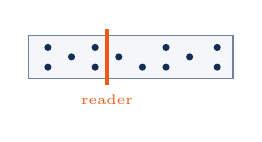
\begin{tikzpicture}
  \draw[draw=DeepBlue!60, fill=LightGray] (0,0) rectangle (2.6,0.55);
  \foreach \x/\y in {0.25/0.15,0.25/0.4,0.55/0.28,0.85/0.15,0.85/0.4,1.15/0.28,1.45/0.15,1.75/0.4,1.75/0.15,2.05/0.28,2.4/0.15,2.4/0.4}
    {\fill[DeepBlue] (\x,\y) circle (0.045);}
  \draw[AccentOrange, very thick] (1.0,-0.08) -- (1.0,0.63);
  \node[font=\tiny, text=AccentOrange, anchor=north] at (1.0,-0.08) {reader};
\end{tikzpicture}}

\newcommand{\diagMemStackSmall}{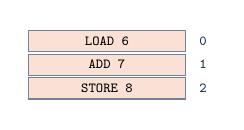
\begin{tikzpicture}
  \node[smallcell, fill=AccentOrange!18, minimum width=2.0cm] at (0,0.3) {LOAD 6};
  \node[smallcell, fill=AccentOrange!18, minimum width=2.0cm] at (0,0) {ADD 7};
  \node[smallcell, fill=AccentOrange!18, minimum width=2.0cm] at (0,-0.3) {STORE 8};
  \node[addr, font=\ttfamily\tiny, anchor=west] at (1.05,0.3) {0};
  \node[addr, font=\ttfamily\tiny, anchor=west] at (1.05,0) {1};
  \node[addr, font=\ttfamily\tiny, anchor=west] at (1.05,-0.3) {2};
\end{tikzpicture}}

\newcommand{\diagTwoMem}{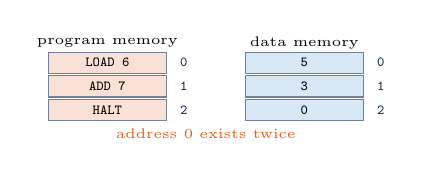
\begin{tikzpicture}
  \node[font=\tiny] at (0,0.55) {program memory};
  \node[font=\tiny] at (2.5,0.55) {data memory};
  \node[smallcell, fill=AccentOrange!18, minimum width=1.5cm] at (0,0.3) {LOAD 6};
  \node[smallcell, fill=AccentOrange!18, minimum width=1.5cm] at (0,0) {ADD 7};
  \node[smallcell, fill=AccentOrange!18, minimum width=1.5cm] at (0,-0.3) {HALT};
  \node[smallcell, fill=StorageBlue!18, minimum width=1.5cm] at (2.5,0.3) {5};
  \node[smallcell, fill=StorageBlue!18, minimum width=1.5cm] at (2.5,0) {3};
  \node[smallcell, fill=StorageBlue!18, minimum width=1.5cm] at (2.5,-0.3) {0};
  \foreach \i in {0,1,2} {
    \node[addr, font=\ttfamily\tiny, anchor=west] at (0.8,{0.3-0.3*\i}) {\i};
    \node[addr, font=\ttfamily\tiny, anchor=west] at (3.3,{0.3-0.3*\i}) {\i};
  }
  \node[font=\tiny, text=AccentOrange] at (1.25,-0.6) {address 0 exists twice};
\end{tikzpicture}}

\newcommand{\diagOneMem}{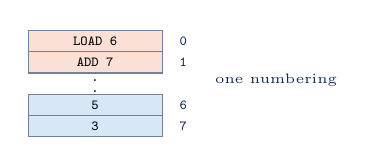
\begin{tikzpicture}
  \node[smallcell, fill=AccentOrange!18, minimum width=1.7cm] (o0) at (0,0.5) {LOAD 6};
  \node[smallcell, fill=AccentOrange!18, minimum width=1.7cm] at (0,0.23) {ADD 7};
  \node[smallcell, draw=none, minimum width=1.7cm] at (0,-0.04) {$\vdots$};
  \node[smallcell, fill=StorageBlue!18, minimum width=1.7cm] at (0,-0.31) {5};
  \node[smallcell, fill=StorageBlue!18, minimum width=1.7cm] at (0,-0.58) {3};
  \node[addr, font=\ttfamily\tiny, anchor=west] at (0.95,0.5) {0};
  \node[addr, font=\ttfamily\tiny, anchor=west] at (0.95,0.23) {1};
  \node[addr, font=\ttfamily\tiny, anchor=west] at (0.95,-0.31) {6};
  \node[addr, font=\ttfamily\tiny, anchor=west] at (0.95,-0.58) {7};
  \node[font=\tiny, text=DeepBlue, anchor=west] at (1.4,0) {one numbering};
\end{tikzpicture}}

\newcommand{\diagDecimal}{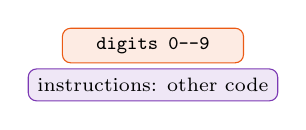
\begin{tikzpicture}
  \node[draw=AccentOrange, fill=AccentOrange!12, rounded corners=3pt, font=\ttfamily\scriptsize, minimum height=0.4cm,
    minimum width=2.3cm] at (0,0.28) {digits 0--9};
  \node[draw=ProgramPurple, fill=ProgramPurple!12, rounded corners=3pt, font=\scriptsize, minimum height=0.4cm,
    minimum width=2.3cm] at (0,-0.22) {instructions: other code};
\end{tikzpicture}}

\newcommand{\diagBinary}{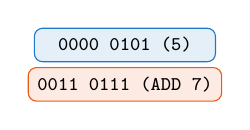
\begin{tikzpicture}
  \node[draw=StorageBlue, fill=StorageBlue!12, rounded corners=3pt, font=\ttfamily\scriptsize, minimum height=0.4cm,
    minimum width=2.3cm] at (0,0.28) {0000 0101 (5)};
  \node[draw=AccentOrange, fill=AccentOrange!12, rounded corners=3pt, font=\ttfamily\scriptsize, minimum height=0.4cm,
    minimum width=2.3cm] at (0,-0.22) {0011 0111 (ADD 7)};
\end{tikzpicture}}

\newcommand{\diagParallel}{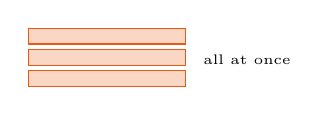
\begin{tikzpicture}
  \foreach \k in {0,1,2} {\draw[fill=AccentOrange!25, draw=AccentOrange] (0,{0.6-0.27*\k}) rectangle (2.0,{0.4-0.27*\k});}
  \node[font=\tiny, anchor=west] at (2.1,0.2) {all at once};
\end{tikzpicture}}

\newcommand{\diagDataflow}{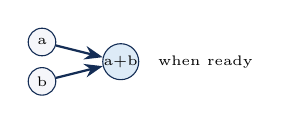
\begin{tikzpicture}[>=Stealth]
  \node[circle, draw=DeepBlue, fill=LightGray, minimum size=0.35cm, inner sep=0pt, font=\tiny] (a) at (0,0.3) {a};
  \node[circle, draw=DeepBlue, fill=LightGray, minimum size=0.35cm, inner sep=0pt, font=\tiny] (b) at (0,-0.2) {b};
  \node[circle, draw=DeepBlue, fill=StorageBlue!15, minimum size=0.4cm, inner sep=0pt, font=\tiny] (c) at (1.0,0.05) {a+b};
  \draw[->, thick, DeepBlue] (a) -- (c); \draw[->, thick, DeepBlue] (b) -- (c);
  \node[font=\tiny, anchor=west] at (1.35,0.05) {when ready};
\end{tikzpicture}}

\newcommand{\diagSequential}{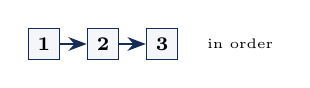
\begin{tikzpicture}[>=Stealth]
  \foreach \k in {1,2,3} {\node[draw=DeepBlue, fill=LightGray, minimum size=0.4cm, inner sep=0pt, font=\scriptsize\bfseries]
    (s\k) at ({0.75*\k-0.75},0.05) {\k};}
  \draw[->, thick, DeepBlue] (s1) -- (s2); \draw[->, thick, DeepBlue] (s2) -- (s3);
  \node[font=\tiny, anchor=west] at (1.95,0.05) {in order};
\end{tikzpicture}}

\newcommand{\diagMonolith}{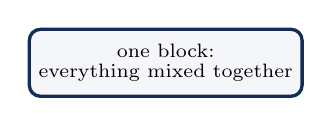
\begin{tikzpicture}
  \node[draw=DeepBlue, very thick, rounded corners=4pt, fill=LightGray, minimum width=2.6cm, minimum height=0.85cm,
    font=\scriptsize, align=center] {one block:\\[-1pt]everything mixed together};
\end{tikzpicture}}

\newcommand{\diagUnits}{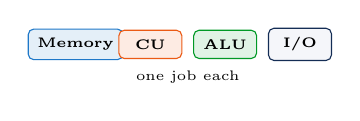
\begin{tikzpicture}
  \node[draw=StorageBlue, fill=StorageBlue!12, rounded corners=2pt, font=\tiny\bfseries, minimum width=0.8cm, minimum height=0.36cm] at (0,0.22) {Memory};
  \node[draw=AccentOrange, fill=AccentOrange!12, rounded corners=2pt, font=\tiny\bfseries, minimum width=0.8cm, minimum height=0.36cm] at (0.95,0.22) {CU};
  \node[draw=mygreen, fill=mygreen!12, rounded corners=2pt, font=\tiny\bfseries, minimum width=0.8cm, minimum height=0.36cm] at (1.9,0.22) {ALU};
  \node[draw=DeepBlue, fill=LightGray, rounded corners=2pt, font=\tiny\bfseries, minimum width=0.8cm, minimum height=0.36cm] at (2.85,0.22) {I/O};
  \node[font=\tiny] at (1.425,-0.2) {one job each};
\end{tikzpicture}}

% ---------- helpers for the CPU section ----------
\tikzset{
  reg/.style={draw=orange!80!black, very thick, fill=yellow!25, rounded corners=2pt,
    minimum width=1.95cm, minimum height=0.55cm, inner sep=2pt, font=\ttfamily\scriptsize, align=center},
  cpuunit/.style={very thick, rounded corners=3pt, minimum width=1.2cm, minimum height=0.6cm,
    inner sep=2pt, font=\scriptsize\bfseries, align=center},
  hot/.style={fill=AccentOrange!45, draw=AccentOrange, very thick},
  hotdata/.style={fill=StorageBlue!40, draw=StorageBlue, very thick},
  hotalu/.style={fill=mygreen!18, line width=1.6pt},
  fetcharrow/.style={-{Stealth}, very thick, DeepBlue, rounded corners=3pt},
  dataarrow/.style={-{Stealth}, very thick, DeepBlue, rounded corners=3pt},
  steplabel/.style={font=\tiny\bfseries, fill=white, inner sep=1pt},
}
% memory with the running example
% #1 highlighted instruction (0-3, -1 = none)  #2 text of cell 8  #3 highlighted data cell (6-8, 0 = none)
\newcommand{\mempanel}[3]{%
  \node[font=\scriptsize\bfseries, text=StorageBlue] at (0,1.8) {Memory};
  \foreach \i/\t in {0/{0001 0110\ \ LOAD 6},1/{0011 0111\ \ ADD 7},2/{0010 1000\ \ STORE 8},3/{0111 0000\ \ HALT}} {
    \ifnum\i=#1
      \node[instrcell, minimum width=2.9cm, hot] (m\i) at (0,{1.35-0.45*\i}) {\t};
    \else
      \node[instrcell, minimum width=2.9cm] (m\i) at (0,{1.35-0.45*\i}) {\t};
    \fi
    \node[addr, anchor=east] at (-1.5,{1.35-0.45*\i}) {\i};
  }
  \node[memcell, draw=none, minimum width=2.9cm] at (0,-0.45) {$\vdots$};
  \foreach \i/\t/\y in {6/{0000 0101\ \ (5)}/-0.9,7/{0000 0011\ \ (3)}/-1.35,8/{#2}/-1.8} {
    \ifnum\i=#3
      \node[datacell, minimum width=2.9cm, hotdata] (m\i) at (0,\y) {\t};
    \else
      \node[datacell, minimum width=2.9cm] (m\i) at (0,\y) {\t};
    \fi
    \node[addr, anchor=east] at (-1.5,\y) {\i};
  }
}
% the CPU, built up step by step
% #1 level: 0 empty, 1 +PC, 2 +IR, 3 +AC, 4 +ALU, 5 +CU   #2 PC   #3 IR   #4 AC   #5 extra ALU style
\newcommand{\cpupanel}[5]{%
  \node[draw=DeepBlue, very thick, rounded corners=6pt, fill=DeepBlue!6, minimum width=4.65cm,
    minimum height=3.85cm, anchor=west] (cpu) at (2.45,-0.2) {};
  \node[font=\scriptsize\bfseries, text=DeepBlue, anchor=north west] at ([shift={(0.1,-0.06)}]cpu.north west) {CPU};
  \ifnum#1>0 \node[reg] (pc) at (3.65,0.95) {\textbf{PC}\ \ #2}; \fi
  \ifnum#1>1 \node[reg] (ir) at (3.65,0.0) {\textbf{IR}\\[-1pt]#3}; \fi
  \ifnum#1>2 \node[reg] (ac) at (3.65,-1.05) {\textbf{AC}\ \ #4}; \fi
  \ifnum#1>3 \node[cpuunit, draw=mygreen, fill=mygreen!18, #5] (alu) at (6.3,-1.05)
    {\textcolor{mygreen!60!black}{\faCalculator}\\[-1pt]ALU}; \fi
  \ifnum#1>4 \node[cpuunit, draw=AccentOrange, fill=AccentOrange!18] (cu) at (6.3,0.5)
    {\textcolor{AccentOrange}{\faCogs}\\[-1pt]CU}; \fi
}
% explanation slide: #1 title, #2 tikz body (memory + CPU), #3 right-hand column
\newcommand{\explainframe}[3]{%
\begin{frame}{#1}
  \begin{columns}[c,onlytextwidth]
    \column{0.58\textwidth}
      \centering
      \begin{tikzpicture}[>=Stealth, scale=0.92, every node/.append style={transform shape}]
        #2
      \end{tikzpicture}
    \column{0.4\textwidth}
      #3
  \end{columns}
\end{frame}}
% boxes for the right-hand column
\newcommand{\defbox}[1]{%
  \begin{beamercolorbox}[rounded=true,sep=0.1cm,wd=\linewidth]{block body example}
    \footnotesize #1
  \end{beamercolorbox}\vspace{0.06cm}}
\newcommand{\stepbox}[2]{%
  \begin{beamercolorbox}[rounded=true,sep=0.09cm,wd=\linewidth]{block body}
    \footnotesize\textbf{#1}\\ #2
  \end{beamercolorbox}\vspace{0.06cm}}
\newcommand{\phasename}[1]{%
  {\centering\footnotesize Name of this phase:\ \colorbox{DeepBlue}{\textcolor{white}{\textbf{#1}}}\par}}
% small tag above the CPU box: which instruction is being executed
\newcommand{\executing}[1]{%
  \node[font=\scriptsize\bfseries, text=AccentOrange, anchor=south east] at ([yshift=1pt]cpu.north east)
    {Executing: \texttt{#1}};}
\newcommand{\statebox}[1]{%
  {\centering\scriptsize\textcolor{DeepBlue}{\textbf{State:}}\ #1\par}}

\lstset{
  language=Python,
  basicstyle=\color{VSText}\ttfamily\footnotesize,
  keywordstyle=\color{VSPurple}\bfseries,
  stringstyle=\color{VSString},
  commentstyle=\color{VSComment}\itshape,
  numbers=left,
  numberstyle=\tiny\color{gray},
  stepnumber=1,
  breaklines=true,
  showstringspaces=false,
  xleftmargin=15pt,
  xrightmargin=5pt,
  frame=none
}

% MARIE assembly: line numbers start at 0, so a line number equals the memory address
\lstdefinelanguage{MARIE}{
  morekeywords={Load,Store,Add,Subt,Input,Output,Halt,Jump,Skipcond,DEC,HEX,ADR,LoadI,StoreI,AddI,JumpI,JnS,Clear,LoadImmi},
  sensitive=false,
  comment=[l]{/},
}
\lstdefinestyle{marie}{language=MARIE, firstnumber=0, basicstyle=\color{VSText}\ttfamily\scriptsize,
  keywordstyle=\color{VSBlue}\bfseries, commentstyle=\color{VSComment}\itshape,
  columns=fixed, basewidth=0.52em, keepspaces=true, breaklines=false, xleftmargin=12pt}

\BeforeBeginEnvironment{lstlisting}{%
  \begin{beamercolorbox}[rounded=true,sep=2mm,wd=\linewidth]{vscodelisting}%
  
\begin{tikzpicture}
    \fill[MacRed] (0,0) circle (3pt);
    \fill[MacYellow] (0.35,0) circle (3pt);
    \fill[MacGreen] (0.70,0) circle (3pt);
  \end{tikzpicture}%
  \vspace{-0.2cm}%
}
\AfterEndEnvironment{lstlisting}{\end{beamercolorbox}}

% =====================================================================
%  Day 2 helpers
% =====================================================================

% ---------- MARIE datapath, drawn like the Data Path view of MARIE.js ----------
% \busdiagram[values]{source}{destination}{extra TikZ}
%   source (Read, blue) and destination (Write, red): ir, out, in, ac, mbr, pc, mar, mem, none
%   values: ir=, out=, in=, ac=, mbr=, pc=, mar=, mem= (contents of M[MAR]), step= (0-7, -1 = none)
\definecolor{ReadBlue}{RGB}{30,150,230}
\definecolor{WriteRed}{RGB}{220,50,80}
\definecolor{BusGreen}{RGB}{60,170,110}
\tikzset{
  dpreg/.style={draw=DeepBlue!80, thick, fill=white, minimum width=1.1cm, minimum height=0.46cm,
    inner sep=1pt, font=\ttfamily\scriptsize},
  dpname/.style={font=\tiny, text=DeepBlue!80, above=0pt, inner sep=1pt},
  dpwire/.style={thin, DeepBlue!18},
  dpmem/.style={draw=StorageBlue, very thick, fill=StorageBlue!12, rounded corners=3pt,
    minimum width=1.3cm, minimum height=0.95cm, font=\scriptsize\bfseries, align=center},
  srcreg/.style={draw=ReadBlue, line width=1.6pt},
  dstreg/.style={draw=WriteRed, line width=1.6pt},
}
\pgfkeys{/dp/.is family, /dp,
  ir/.initial={0000}, out/.initial={0000}, in/.initial={0000}, ac/.initial={0000},
  mbr/.initial={0000}, pc/.initial={000}, mar/.initial={000}, mem/.initial={0000},
  step/.initial={-1}}
\newcommand{\dpv}[1]{\pgfkeysvalueof{/dp/#1}}
\newcommand{\busdiagram}[4][]{%
  \begingroup
  \pgfkeys{/dp, ir=0000, out=0000, in=0000, ac=0000, mbr=0000, pc=000, mar=000, mem=0000, step=-1, #1}%
  \begin{tikzpicture}[>=Stealth]
    \tikzset{bd-mem/.style={}, bd-mar/.style={}, bd-pc/.style={}, bd-mbr/.style={},
      bd-ac/.style={}, bd-ir/.style={}, bd-in/.style={}, bd-out/.style={}, bd-none/.style={}}
    \tikzset{bd-#2/.style={srcreg}}
    \tikzset{bd-#3/.style={dstreg}}
    % ----- control unit -----
    \node[draw=DeepBlue!80, thick, fill=white, minimum width=1.3cm, minimum height=2.95cm,
      anchor=north west] (cu) at (-2.4,2.0) {};
    \node[font=\tiny, text=DeepBlue, anchor=north west, below=1pt] at (cu.south west) {Control unit};
    \node[font=\tiny, text=DeepBlue!80, anchor=east] at (-1.15,1.75) {Read};
    \node[font=\tiny, text=DeepBlue!80, anchor=east] at (-1.15,-0.6) {Write};
    \node[font=\tiny, text=DeepBlue!80, anchor=east] at (-1.15,0.05) {AC<0};
    \node[font=\tiny, text=DeepBlue!80, anchor=east] at (-1.15,-0.15) {AC=0};
    \node[font=\tiny, text=DeepBlue!80] at (-2.0,1.3) {Step};
    \foreach \k in {0,...,7} {
      \pgfmathtruncatemacro{\cur}{\dpv{step}}
      \ifnum\k=\cur
        \fill[ReadBlue] (-2.0,{1.1-0.15*\k}) circle (0.065);
      \else
        \fill[DeepBlue!30] (-2.0,{1.1-0.15*\k}) circle (0.035);
      \fi
    }
    % ----- memory -----
    \node[draw=DeepBlue!80, thick, fill=white, minimum width=1.5cm, minimum height=2.95cm,
      anchor=north west, bd-mem] (mem) at (10.4,2.0) {};
    \node[font=\tiny, text=DeepBlue, anchor=north west, below=1pt] at (mem.south west) {Main memory};
    \node[font=\ttfamily\tiny, text=DeepBlue!80] at (11.15,0.75) {M[MAR]};
    \node[font=\ttfamily\scriptsize] at (11.15,0.5) {\dpv{mem}};
    % ----- faint control wires (one Read and one Write wire per device) -----
    \draw[dpwire] (-1.1,1.75) -- (10.4,1.75);
    \draw[dpwire] (-1.1,-0.6) -- (10.4,-0.6);
    \foreach \x in {0.6,2.0,3.4,4.8,6.2,7.6,9.0} {
      \draw[dpwire] (\x-0.25,1.75) -- (\x-0.25,1.18);
      \draw[dpwire] (\x+0.3,-0.6) -- (\x+0.3,0.72);
    }
    % ----- bus (drawn first, registers on top) -----
    \foreach \x in {0.6,2.0,3.4,4.8,6.2,7.6,9.0}
      \draw[line width=2.6pt, BusGreen] (\x,0.72) -- (\x,-0.35);
    \draw[line width=2.6pt, BusGreen] (0.6-0.045,-0.35) -- (10.4,-0.35);
    % ----- ALU between AC and MBR, with its links and the flag wires to the CU -----
    \draw[thin, DeepBlue!40] (4.45,0.05) -- (-1.1,0.05);
    \draw[thin, DeepBlue!40] (4.45,-0.15) -- (-1.1,-0.15);
    \draw[thick, DeepBlue!70, fill=white] (5.0,0.47) -- (5.42,0.47) -- (5.5,0.37) -- (5.58,0.47) -- (6.0,0.47)
      -- (5.72,0.05) -- (5.28,0.05) -- cycle;
    \node[font=\tiny, text=DeepBlue!80] at (5.5,0.22) {ALU};
    \draw[thick, DeepBlue!60] (5.2,0.72) -- (5.2,0.47);
    \draw[thick, DeepBlue!60] (5.8,0.72) -- (5.8,0.47);
    \draw[thick, DeepBlue!60] (5.5,0.05) -- (5.5,-0.1) -- (4.45,-0.1) |- (4.45,0.72);
    % ----- registers -----
    \foreach \n/\x/\lab in {ir/0.6/IR, out/2.0/OUT, in/3.4/IN, ac/4.8/AC, mbr/6.2/MBR, pc/7.6/PC, mar/9.0/MAR} {
      \node[dpreg, bd-\n] (\n) at (\x,0.95) {\dpv{\n}};
      \node[dpname] at (\n.north) {\lab};
      \coordinate (\n-port) at (\n.south);
      \coordinate (\n-bus) at (\x,-0.35);
    }
    \coordinate (mem-port) at (10.4,-0.35);
    \coordinate (mem-bus) at (10.4,-0.35);
    % IR is decoded by the CU; MAR selects the memory cell
    \draw[thick, BusGreen, -{Stealth}] (ir.west) -- (-1.1,0.95);
    \draw[thick, BusGreen, -{Stealth}] (mar.east) -- (10.4,0.95);
    % ----- active Read and Write signals -----
    \ifstrequal{#2}{none}{}{%
      \ifstrequal{#2}{mem}
        {\draw[line width=1.3pt, ReadBlue, -{Stealth}] (-1.1,1.75) -- (10.4,1.75);}
        {\draw[line width=1.3pt, ReadBlue, -{Stealth}] (-1.1,1.75) -| ($(#2.north)+(-0.25,0)$);}}
    \ifstrequal{#3}{none}{}{%
      \ifstrequal{#3}{mem}
        {\draw[line width=1.3pt, WriteRed, -{Stealth}] (-1.1,-0.6) -- (10.4,-0.6);}
        {\draw[line width=1.3pt, WriteRed, -{Stealth}] (-1.1,-0.6) -| ($(#3.south)+(0.3,0)$);}}
    % ----- the value travelling along the bus -----
    \ifstrequal{#2}{none}{}{\ifstrequal{#3}{none}{}{%
      \draw[line width=3pt, BusGreen] (#2-port) -- (#2-bus) -- (#3-bus) -- (#3-port);
      \draw[line width=1.5pt, white, dash pattern=on 1.5pt off 1.5pt] (#2-port) -- (#2-bus) -- (#3-bus) -- (#3-port);}}
    #4
  \end{tikzpicture}%
  \endgroup}

% legend for the colours of the data path
\newcommand{\dplegend}{%
  {\tiny\textcolor{ReadBlue}{\rule{0.25cm}{0.2cm}}\ \textbf{Read}: puts its value on the bus
  \qquad\textcolor{WriteRed}{\rule{0.25cm}{0.2cm}}\ \textbf{Write}: stores the value from the bus
  \qquad\tikz[baseline=-0.6ex]{\draw[line width=3pt, BusGreen] (0,0) -- (0.5,0);\draw[line width=1.5pt, white, dash pattern=on 1.5pt off 1.5pt] (0,0) -- (0.5,0);}\ the value travelling on the bus}}

% one step of an instruction: data path on top, explanation below
% #1 title, #2 source, #3 destination, #4 values (keys), #5 explanation
\newcommand{\stepframe}[5]{%
\begin{frame}{#1}
  \begin{center}
    \resizebox{0.8\textwidth}{!}{\busdiagram[#4]{#2}{#3}{}}\\[0.02cm]
    \dplegend
  \end{center}
  \vspace{-0.1cm}
  \begin{center}
    \begin{minipage}{0.8\textwidth}
      #5
    \end{minipage}
  \end{center}
\end{frame}}

% ---------- timeline of clock steps ----------
% #1 fetch steps, #2 execute steps, #3 label on the right
\newcommand{\steptimeline}[3]{%
  \begin{tikzpicture}
    \foreach \i in {1,...,#1}
      \node[draw=white, fill=StorageBlue!75, text=white, font=\tiny\bfseries, minimum width=0.62cm,
        minimum height=0.45cm, inner sep=0pt] at ({0.62*(\i-1)},0) {T\the\numexpr\i-1\relax};
    \foreach \i in {1,...,#2}
      \node[draw=white, fill=AccentOrange, text=white, font=\tiny\bfseries, minimum width=0.62cm,
        minimum height=0.45cm, inner sep=0pt] at ({0.62*(#1+\i-1)},0) {T\the\numexpr#1+\i-1\relax};
    \node[anchor=west, font=\scriptsize] at ({0.62*(#1+#2)-0.25},0) {#3};
  \end{tikzpicture}}

% legend for the timeline colours
\newcommand{\timelinelegend}{%
  {\tiny\textcolor{StorageBlue!75}{\rule{0.25cm}{0.2cm}}\ fetch
  \qquad\textcolor{AccentOrange}{\rule{0.25cm}{0.2cm}}\ execute}}

% ---------- small pieces for the addressing-mode slides ----------
\tikzset{
  mcell/.style={draw=DeepBlue!60, minimum width=1.5cm, minimum height=0.42cm, inner sep=1pt,
    font=\ttfamily\scriptsize, align=center, fill=StorageBlue!15},
  mcellhot/.style={mcell, fill=StorageBlue!45, draw=StorageBlue, very thick},
  mcellptr/.style={mcell, fill=ProgramPurple!18, draw=ProgramPurple, very thick},
  instrbox/.style={draw=AccentOrange, very thick, fill=AccentOrange!15, rounded corners=2pt,
    minimum height=0.5cm, inner sep=3pt, font=\ttfamily\scriptsize},
  ptrarrow/.style={-{Stealth}, very thick, DeepBlue},
  valarrow/.style={-{Stealth}, very thick, DeepBlue},
}

% task header box (same look as on Day 1)
% #1 form and time, #2 short instruction
\newcommand{\taskhead}[2]{%
  \begin{beamercolorbox}[rounded=true,sep=0.12cm,wd=\linewidth]{block body example}
    \small\textbf{#1}\\[0.04cm]
    \footnotesize #2
  \end{beamercolorbox}\vspace{0.1cm}}

% highlighted key message at the bottom of a slide
\newcommand{\keymsg}[1]{%
  \begin{beamercolorbox}[rounded=true,sep=0.1cm,wd=\textwidth]{block body example}
    \centering\footnotesize #1
  \end{beamercolorbox}}

% register transfer written in text: \mo{MAR}{PC} gives MAR <- PC
\newcommand{\mo}[2]{\texttt{#1\,$\leftarrow$\,#2}}

% plain listings (x86, RISC-V) without Python highlighting
\lstdefinelanguage{plain}{}
\lstdefinestyle{asm}{language=plain, basicstyle=\color{VSText}\ttfamily\scriptsize, numbers=none,
  columns=fixed, basewidth=0.52em, keepspaces=true, xleftmargin=6pt}

% =====================================================================
%  Day 3 helpers
% =====================================================================

\usetikzlibrary{patterns}
\usepackage{multirow}
% ---------- RISC-V listings ----------
\lstdefinestyle{rv}{language=RISCV, basicstyle=\color{VSText}\ttfamily\scriptsize, numbers=none,
  keywordstyle=\color{VSBlue}\bfseries, keywordstyle={[2]\color{VSPurple}\bfseries},
  commentstyle=\color{VSComment}\itshape,
  columns=fixed, basewidth=0.52em, keepspaces=true, breaklines=false, xleftmargin=6pt}
\lstdefinestyle{rvnum}{style=rv, numbers=left, firstnumber=1, xleftmargin=14pt}

% ---------- colours of the five pipeline stages (the same all day) ----------
\colorlet{cIF}{AccentOrange}
\colorlet{cID}{ProgramPurple}
\colorlet{cEX}{mygreen}
\colorlet{cMEM}{StorageBlue}
\colorlet{cWB}{DeepBlue}

% ---------- pipeline diagrams ----------
% cell size (cm)
\def\pw{0.74}
\def\ph{0.46}
\tikzset{
  pcell/.style={minimum width=\pw cm, minimum height=\ph cm, inner sep=0pt, draw=white,
    font=\scriptsize\bfseries, text=white},
  pst-IF/.style={pcell, fill=cIF},
  pst-ID/.style={pcell, fill=cID},
  pst-EX/.style={pcell, fill=cEX},
  pst-MEM/.style={pcell, fill=cMEM},
  pst-WB/.style={pcell, fill=cWB},
  pst-B/.style={pcell, fill=gray!25, text=gray!70, font=\tiny},
  pst-X/.style={pcell, fill=MacRed!20, text=MacRed},
  pst-N/.style={pcell, fill=none, draw=none},
  pst-E/.style={pcell, fill=gray!10},
  plab/.style={anchor=east, font=\ttfamily\footnotesize, inner sep=1pt},
}
% one row of a pipeline diagram
% #1 row (0 = top), #2 first cycle (1-based), #3 comma list of IF, ID, EX, MEM, WB, B (bubble), X (flushed), N (empty)
\newcommand{\prow}[3]{%
  \foreach \s [count=\k from 0] in {#3} {%
    \node[pst-\s] at ({(#2+\k-1)*\pw}, {-(#1)*\ph}) {%
      \expandafter\ifstrequal\expandafter{\s}{B}{bubble}{%
      \expandafter\ifstrequal\expandafter{\s}{X}{$\times$}{%
      \expandafter\ifstrequal\expandafter{\s}{N}{}{\expandafter\ifstrequal\expandafter{\s}{E}{}{\s}}}}};
  }}
% label of a row
\newcommand{\plabel}[2]{\node[plab] at ({-0.5*\pw-0.05}, {-(#1)*\ph}) {#2};}
% cycle numbers above the diagram: #1 number of cycles
\newcommand{\pcycles}[1]{%
  \foreach \c in {1,...,#1}
    \node[font=\scriptsize, text=DeepBlue!70] at ({(\c-1)*\pw}, {0.8*\ph}) {\c};
  \node[font=\scriptsize, text=DeepBlue!70, anchor=east] at ({-0.5*\pw-0.05}, {0.8*\ph}) {cycle};}
% highlight one column: #1 cycle, #2 number of rows, #3 colour
\newcommand{\pcolumn}[3]{%
  \draw[#3, very thick, rounded corners=2pt]
    ({(#1-1.5)*\pw}, {0.5*\ph}) rectangle ({(#1-0.5)*\pw}, {-(#2-0.5)*\ph});}

% legend of stage colours
\newcommand{\stagelegend}{%
  {\tiny
  \textcolor{cIF}{\rule{0.25cm}{0.2cm}}\,IF fetch\quad
  \textcolor{cID}{\rule{0.25cm}{0.2cm}}\,ID decode\quad
  \textcolor{cEX}{\rule{0.25cm}{0.2cm}}\,EX execute\quad
  \textcolor{cMEM}{\rule{0.25cm}{0.2cm}}\,MEM memory\quad
  \textcolor{cWB}{\rule{0.25cm}{0.2cm}}\,WB write back}}

% ---------- stage boxes ----------
\tikzset{
  stagebox/.style={very thick, rounded corners=4pt, minimum width=1.9cm, minimum height=0.8cm,
    align=center, font=\small\bfseries, drop shadow},
  gbar/.style={minimum height=0.36cm, inner sep=0pt, draw=white, font=\tiny\bfseries, text=white},
  gempty/.style={minimum height=0.36cm, inner sep=0pt, draw=gray!50, dashed, font=\tiny, text=gray!60},
  unit/.style={draw=DeepBlue, very thick, fill=white, rounded corners=3pt, align=center,
    font=\scriptsize\bfseries, inner sep=2pt},
}

% ---------- a simple RISC-V datapath ----------
% #1 extra TikZ drawn on top (nodes: pc, imem, rf, alu, dmem, mux, cu, add4)
\newcommand{\rvdatapath}[1]{%
  \begin{tikzpicture}[>=Stealth, font=\scriptsize]
    % stage labels
    \foreach \x/\n/\c in {0.9/IF/cIF, 4.2/ID/cID, 6.6/EX/cEX, 9.0/MEM/cMEM, 10.9/WB/cWB}
      \node[fill=\c, text=white, rounded corners=2pt, font=\tiny\bfseries, minimum width=0.9cm] at (\x,2.35) {\n};
    % units
    \node[unit, minimum width=0.6cm, minimum height=1.0cm] (pc) at (0,0) {PC};
    \node[unit, minimum width=1.5cm, minimum height=1.6cm] (imem) at (1.8,0) {Instruction\\memory};
    \node[unit, minimum width=1.5cm, minimum height=1.8cm] (rf) at (4.2,0) {Register\\file};
    \draw[DeepBlue, very thick, fill=white] (6.2,0.9) -- (7.0,0.45) -- (7.0,-0.45) -- (6.2,-0.9) -- (6.2,-0.25)
      -- (6.4,0) -- (6.2,0.25) -- cycle;
    \node[font=\scriptsize\bfseries] (alu) at (6.68,0) {ALU};
    \coordinate (aluin1) at (6.2,0.55); \coordinate (aluin2) at (6.2,-0.55); \coordinate (aluout) at (7.0,0);
    \node[unit, minimum width=1.5cm, minimum height=1.6cm] (dmem) at (9.0,0) {Data\\memory};
    \node[unit, minimum width=0.45cm, minimum height=1.2cm, rounded corners=6pt, font=\tiny] (mux) at (10.9,0) {M\\U\\X};
    \node[unit, minimum width=1.3cm, minimum height=0.5cm, draw=DeepBlue!60, text=DeepBlue!80] (add4) at (0.9,1.55) {$+4$};
    \node[unit, minimum width=2.2cm, minimum height=0.5cm, draw=gray, text=gray] (cu) at (4.2,-1.85) {Control unit};
    % wires
    \draw[->, thick] (pc) -- (imem);
    \draw[->, thick] (imem) -- node[above, font=\tiny] {instruction} (rf);
    \draw[->, thick] ([yshift=0.55cm]rf.east) -- (aluin1);
    \draw[->, thick] ([yshift=-0.55cm]rf.east) -- (aluin2);
    \draw[->, thick] (aluout) -- node[above, font=\tiny] {address} ([yshift=0cm]dmem.west);
    \draw[->, thick] ([yshift=-0.55cm]dmem.east) -- ([yshift=-0.4cm]mux.west);
    \draw[->, thick] (7.3,0) |- (7.3,-1.1) -| (10.3,-1.1) |- ([yshift=0.4cm]mux.west);
    \draw[->, thick] (mux.east) -- ++(0.3,0) |- (11.2,2.0) -| node[pos=0.25, above, font=\tiny] {write back} (4.2,0.9);
    \draw[->, thick, DeepBlue!60] (pc.north) |- (add4.west);
    \draw[->, thick, DeepBlue!60] (add4.east) -- ++(0.35,0) |- (-0.6,1.95) |- (pc.west);
    \draw[->, dashed, gray] (cu.north) -- (rf.south);
    \draw[->, dashed, gray] (cu.east) -| (dmem.south);
    \draw[->, dashed, gray] (cu.east) -| (mux.south);
    #1
  \end{tikzpicture}}

% ---------- Ripes window (schematic; replace with a real screenshot if you like) ----------
\newcommand{\ripeswindow}{%
  \begin{tikzpicture}[font=\tiny]
    \draw[DeepBlue, very thick, fill=white, rounded corners=4pt] (0,0) rectangle (9,5.4);
    \fill[DeepBlue!10, rounded corners=4pt] (0,5.0) rectangle (9,5.4);
    \fill[MacRed] (0.25,5.2) circle (2.5pt); \fill[MacYellow] (0.5,5.2) circle (2.5pt); \fill[MacGreen] (0.75,5.2) circle (2.5pt);
    \node[font=\tiny\bfseries, text=DeepBlue] at (4.5,5.2) {Ripes};
    % toolbar
    \fill[LightGray] (0,4.55) rectangle (9,5.0);
    \foreach \x/\i in {1.0/\faMicrochip, 1.6/\faStepForward, 2.2/\faPlay, 2.8/\faFastForward, 3.4/\faUndo}
      \node[text=DeepBlue] at (\x,4.77) {\i};
    % side bar
    \fill[DeepBlue!85] (0,0) rectangle (0.5,4.55);
    \foreach \y/\i in {4.1/\faEdit, 3.5/\faMicrochip, 2.9/\faMemory, 2.3/\faTerminal}
      \node[text=white] at (0.25,\y) {\i};
    % editor
    \draw[gray!60, fill=VSDarkBg] (0.65,0.15) rectangle (3.2,4.4);
    \foreach \y/\t in {4.1/lw x5{,} X, 3.8/lw x6{,} Y, 3.5/add x7{,} x5{,} x6, 3.2/addi x7{,} x7{,} -2, 2.9/sw x7{,} Z{,} x28}
      \node[anchor=west, text=VSText, font=\ttfamily\tiny] at (0.75,\y) {\t};
    % processor view
    \draw[gray!60, fill=LightGray] (3.35,1.4) rectangle (7.3,4.4);
    \foreach \x/\c in {3.8/cIF, 4.5/cID, 5.3/cEX, 6.1/cMEM, 6.8/cWB}
      \draw[\c, very thick, fill=\c!15] (\x-0.25,2.3) rectangle (\x+0.25,3.6);
    \draw[->, thick, DeepBlue!60] (3.55,2.95) -- (7.05,2.95);
    \node[font=\tiny, text=DeepBlue] at (5.3,1.85) {datapath};
    % statistics
    \draw[gray!60, fill=white] (3.35,0.15) rectangle (7.3,1.25);
    \node[anchor=west, font=\tiny] at (3.45,0.95) {Cycles: 13};
    \node[anchor=west, font=\tiny] at (3.45,0.7) {Instrs. retired: 8};
    \node[anchor=west, font=\tiny] at (3.45,0.45) {CPI: 1.63 \quad IPC: 0.62};
    % registers
    \draw[gray!60, fill=white] (7.45,0.15) rectangle (8.85,4.4);
    \foreach \k [count=\j from 0] in {x5,x6,x7,x8,x9,x10}
      \node[anchor=west, font=\ttfamily\tiny] at (7.5,{4.1-0.3*\j}) {\k};
    \node[font=\tiny, text=DeepBlue] at (8.15,2.1) {registers};
    % badges
    \node[circle, fill=AccentOrange, text=white, font=\bfseries\scriptsize, inner sep=1.5pt] at (1.9,1.2) {1};
    \node[circle, fill=AccentOrange, text=white, font=\bfseries\scriptsize, inner sep=1.5pt] at (1.35,4.77) {2};
    \node[circle, fill=AccentOrange, text=white, font=\bfseries\scriptsize, inner sep=1.5pt] at (5.3,4.1) {3};
    \node[circle, fill=AccentOrange, text=white, font=\bfseries\scriptsize, inner sep=1.5pt] at (6.95,0.7) {4};
    \node[circle, fill=AccentOrange, text=white, font=\bfseries\scriptsize, inner sep=1.5pt] at (8.15,1.4) {5};
  \end{tikzpicture}}

% small orange number used in running text
\newcommand{\badge}[1]{\tikz[baseline=(b.base)]\node[circle,fill=AccentOrange,text=white,
  inner sep=1.2pt,font=\bfseries\tiny] (b) {#1};}

% =====================================================================
%  Day 4 helpers
% =====================================================================

% ---------- colours of the memory levels (the same all day) ----------
\colorlet{cReg}{AccentOrange}
\colorlet{cCache}{ProgramPurple}
\colorlet{cRAM}{StorageBlue}
\colorlet{cDisk}{DeepBlue!65}
\colorlet{cIO}{mygreen}
\definecolor{HitGreen}{RGB}{39,160,70}
\colorlet{MissRed}{MacRed}
\setbeamercolor{block body answer}{bg=mygreen!10,fg=black}

% ---------- listings ----------
% RISC-V: the Day 3 keywords plus the new ones used today
\lstdefinelanguage{RISCV}{
  morekeywords={lw,sw,add,addi,sub,beq,bne,bnez,beqz,la,li,auipc,nop,ecall},
  morekeywords=[2]{.data,.text,.word,.zero},
  alsoletter={.},
  sensitive=true,
  morecomment=[l]{\#},
}
% C (for the locality examples)
\lstdefinestyle{cc}{language=C, basicstyle=\color{VSText}\ttfamily\scriptsize, numbers=none,
  keywordstyle=\color{VSBlue}\bfseries, commentstyle=\color{VSComment}\itshape,
  columns=fixed, basewidth=0.52em, keepspaces=true, breaklines=false, xleftmargin=6pt,
  moredelim=**[is][\color{MacYellow}\bfseries]{@}{@}}

% ---------- boxes for the memory levels and devices ----------
\tikzset{
  lbox/.style={very thick, rounded corners=4pt, align=center, font=\scriptsize\bfseries, inner sep=3pt},
  cpubox/.style={lbox, draw=DeepBlue, fill=DeepBlue, text=white},
  regbox/.style={lbox, draw=cReg, fill=cReg!15},
  cachebox/.style={lbox, draw=cCache, fill=cCache!12},
  rambox/.style={lbox, draw=cRAM, fill=cRAM!12},
  diskbox/.style={lbox, draw=cDisk, fill=cDisk!15},
  iobox/.style={lbox, draw=cIO, fill=cIO!12},
  dmabox/.style={lbox, draw=AccentOrange, fill=AccentOrange!12},
  osbox/.style={lbox, draw=ProgramPurple, fill=ProgramPurple!10},
  greybox/.style={lbox, draw=gray, fill=gray!8, text=gray!40!black},
  arr/.style={-{Stealth}, very thick, DeepBlue},
  okarr/.style={-{Stealth}, very thick, HitGreen},
  badarr/.style={-{Stealth}, very thick, MissRed},
  smalltxt/.style={font=\tiny, inner sep=1pt},
}

% ---------- design question box (as on the Day 1 dilemma slides) ----------
\newcommand{\designq}[1]{%
  \begin{beamercolorbox}[rounded=true,sep=0.14cm,wd=\textwidth]{block body}
    \centering\small\textbf{Design question:} #1
  \end{beamercolorbox}}
\newcommand{\whichone}{%
  {\centering\small\textcolor{DeepBlue}{\textbf{Which would you choose, and why?}}\par}}

% ---------- question card and answer card ----------
% #1 icon, #2 text
\newcommand{\qcard}[2]{%
  \begin{beamercolorbox}[rounded=true,sep=0.14cm,wd=\linewidth]{block body}
    \centering{\Large\textcolor{AccentOrange}{#1}}\\[0.12cm]
    \footnotesize #2
  \end{beamercolorbox}}
% #1 title, #2 text
\newcommand{\acard}[2]{%
  \begin{beamercolorbox}[rounded=true,sep=0.1cm,wd=\linewidth]{block body answer}
    \footnotesize\textbf{\textcolor{mygreen!70!black}{\faCheck}\ #1}\\ #2
  \end{beamercolorbox}\vspace{0.06cm}}
% red "problem" box
\setbeamercolor{block body problem}{bg=MacRed!10,fg=black}
\newcommand{\probbox}[2]{%
  \begin{beamercolorbox}[rounded=true,sep=0.09cm,wd=\linewidth]{block body problem}
    \footnotesize\textbf{\textcolor{MacRed}{\faExclamationTriangle}\ #1}\\ #2
  \end{beamercolorbox}\vspace{0.06cm}}

% ---------- hits and misses ----------
\def\cw{0.62}
\def\chh{0.42}
\tikzset{
  hmcell/.style={minimum width=\cw cm, minimum height=\chh cm, inner sep=0pt, draw=white,
    font=\scriptsize\bfseries, text=white},
  hm-H/.style={hmcell, fill=HitGreen},
  hm-M/.style={hmcell, fill=MissRed},
  hm-Q/.style={hmcell, fill=gray!10, draw=gray!40, text=gray!60},
  hm-A/.style={hmcell, draw=none, text=DeepBlue, font=\scriptsize\ttfamily\bfseries},
}
% one row of hits and misses: #1 row (0 = top), #2 comma list of H, M, Q (Q = to fill in)
\newcommand{\hmrow}[2]{%
  \foreach \s [count=\k from 0] in {#2} {%
    \node[hm-\s] at ({\k*\cw}, {-(#1)*\chh}) {\expandafter\ifstrequal\expandafter{\s}{Q}{?}{\s}};}}
% the accessed addresses above a row: #1 row, #2 comma list
\newcommand{\hmhead}[2]{%
  \foreach \s [count=\k from 0] in {#2}
    \node[hm-A] at ({\k*\cw}, {-(#1)*\chh}) {\s};}
% label on the left of a row: #1 row, #2 text
\newcommand{\hmlabel}[2]{\node[anchor=east, font=\scriptsize, inner sep=1pt] at ({-0.5*\cw-0.08}, {-(#1)*\chh}) {#2};}
% label on the right of a row: #1 row, #2 number of cells, #3 text
\newcommand{\hmresult}[3]{\node[anchor=west, font=\scriptsize\bfseries, text=DeepBlue, inner sep=1pt]
  at ({(#2-0.5)*\cw+0.12}, {-(#1)*\chh}) {#3};}

% ---------- a small cache (or page table) drawn as a table ----------
\tikzset{
  ctab/.style={draw=DeepBlue!50, minimum height=0.4cm, inner sep=1pt, font=\ttfamily\scriptsize, fill=white},
  ctabh/.style={ctab, fill=DeepBlue, text=white, font=\scriptsize\bfseries},
  ctabhit/.style={fill=HitGreen!25, draw=HitGreen, very thick},
  ctabmiss/.style={fill=MissRed!20, draw=MissRed, very thick},
}
% #1 comma list of line/valid/tag/data ; columns: Line, V, Tag, Data (top-left corner at the origin)
\newcommand{\cachetable}[1]{%
  \node[ctabh, minimum width=0.9cm] at (0,0) {Line};
  \node[ctabh, minimum width=0.7cm] at (0.8,0) {V};
  \node[ctabh, minimum width=1.0cm] at (1.65,0) {Tag};
  \node[ctabh, minimum width=1.6cm] at (2.95,0) {Data};
  \foreach \xa/\xb/\xc/\xd [count=\k from 1] in {#1} {
    \node[ctab, minimum width=0.9cm] (cl\k) at (0,{-0.4*\k}) {\xa};
    \node[ctab, minimum width=0.7cm] (cv\k) at (0.8,{-0.4*\k}) {\xb};
    \node[ctab, minimum width=1.0cm] (ct\k) at (1.65,{-0.4*\k}) {\xc};
    \node[ctab, minimum width=1.6cm] (cd\k) at (2.95,{-0.4*\k}) {\xd};
  }}

% ---------- timelines (polling, interrupts, DMA, bus use) ----------
% #1 y, #2 label on the left, #3 comma list of length/colour/text
\newcommand{\tlbar}[3]{%
  \node[anchor=east, font=\scriptsize\bfseries, text=DeepBlue, align=right] at (-0.1,#1) {#2};
  \gdef\tlx{0}%
  \foreach \tlw/\tlc/\tlt in {#3} {%
    \node[draw=white, fill=\tlc, minimum width=\tlw cm, minimum height=0.42cm, inner sep=0pt,
      anchor=west, font=\tiny\bfseries, text=white] at (\tlx,#1) {\tlt};
    \pgfmathsetmacro{\tlnext}{\tlx+\tlw}%
    \xdef\tlx{\tlnext}%
  }}

% ---------- timing diagrams (buses) ----------
% a digital signal: #1 y, #2 label, #3 comma list of x/level pairs (level 0 or 1), #4 end x
\newcommand{\signal}[4]{%
  \node[anchor=east, font=\scriptsize\bfseries, text=DeepBlue] at (-0.15,{#1+0.2}) {#2};
  \gdef\sgx{0}\gdef\sgl{0}%
  \foreach \sx/\sl in {#3} {%
    \draw[very thick, DeepBlue] (\sgx,{#1+0.4*\sgl}) -- (\sx,{#1+0.4*\sgl}) -- (\sx,{#1+0.4*\sl});
    \xdef\sgx{\sx}\xdef\sgl{\sl}%
  }
  \draw[very thick, DeepBlue] (\sgx,{#1+0.4*\sgl}) -- (#4,{#1+0.4*\sgl});}
% a bus value (address, data): #1 y, #2 label, #3 start x, #4 end x, #5 text, #6 colour
\newcommand{\busval}[6]{%
  \node[anchor=east, font=\scriptsize\bfseries, text=DeepBlue, align=right] at (-0.15,{#1+0.2}) {#2};
  \fill[#6!20] (#3,#1+0.2) -- (#3+0.12,#1+0.4) -- (#4-0.12,#1+0.4) -- (#4,#1+0.2)
    -- (#4-0.12,#1) -- (#3+0.12,#1) -- cycle;
  \draw[very thick, #6] (#3,#1+0.2) -- (#3+0.12,#1+0.4) -- (#4-0.12,#1+0.4) -- (#4,#1+0.2)
    -- (#4-0.12,#1) -- (#3+0.12,#1) -- cycle;
  \node[font=\tiny\bfseries, text=#6!70!black] at ({(#3+#4)/2},{#1+0.2}) {#5};}
% a clock: #1 y, #2 number of periods, #3 period width
\newcommand{\clocksig}[3]{%
  \node[anchor=east, font=\scriptsize\bfseries, text=DeepBlue] at (-0.15,{#1+0.2}) {Bus clock};
  \foreach \c in {1,...,#2} {
    \draw[very thick, DeepBlue] ({(\c-1)*#3},#1) -- ({(\c-1)*#3},{#1+0.4}) -- ({(\c-0.5)*#3},{#1+0.4})
      -- ({(\c-0.5)*#3},#1) -- ({\c*#3},#1);
  }}
% a vertical time marker: #1 x, #2 top y, #3 bottom y, #4 label
\newcommand{\tmark}[4]{%
  \draw[DeepBlue!50, dashed, thick] (#1,#2) -- (#1,#3);
  \node[font=\scriptsize\bfseries, text=AccentOrange, below] at (#1,#3) {#4};}

% ---------- latency bar on a log scale ----------
% #1 row, #2 label, #3 length (cm), #4 colour, #5 text at the end
\newcommand{\latbar}[5]{%
  \node[anchor=east, font=\scriptsize] at (-0.1,{-0.42*#1}) {#2};
  \fill[#4] (0,{-0.42*#1-0.15}) rectangle (#3,{-0.42*#1+0.15});
  \node[anchor=west, font=\scriptsize\bfseries, text=#4!80!black] at (#3+0.05,{-0.42*#1}) {#5};}

% =====================================================================
%  Day 5 helpers
% =====================================================================

% ---------- Arduino C++ listings (@...@ = part to change, shown in yellow) ----------
\lstdefinestyle{ino}{language=C++, basicstyle=\color{VSText}\ttfamily\scriptsize, numbers=none,
  keywordstyle=\color{VSBlue}\bfseries, commentstyle=\color{VSComment}\itshape, stringstyle=\color{VSString},
  columns=fixed, basewidth=0.52em, keepspaces=true, breaklines=false, showstringspaces=false, xleftmargin=6pt,
  morekeywords={uint8_t,uint32_t,IRAM_ATTR,HIGH,LOW,OUTPUT,INPUT_PULLUP,FALLING,hw_timer_t},
  emph={pinMode,digitalWrite,digitalRead,delay,millis,micros,attachInterrupt,digitalPinToInterrupt,
    timerBegin,timerAttachInterrupt,timerAlarm,memcpy,memcmp,memset,esp_async_memcpy,esp_async_memcpy_install},
  emphstyle=\color{VSPurple},
  moredelim=**[is][\color{MacYellow}\bfseries]{@}{@}}
% plain text in a dark box (serial monitor, terminal)
\lstdefinestyle{term}{language=plain, basicstyle=\color{VSText}\ttfamily\scriptsize, numbers=none,
  columns=fixed, basewidth=0.52em, keepspaces=true, xleftmargin=6pt,
  moredelim=**[is][\color{MacYellow}\bfseries]{@}{@}}

% ---------- colours used all day ----------
\colorlet{cWork}{mygreen}
\colorlet{cPoll}{MissRed}
\colorlet{cISR}{AccentOrange}
\colorlet{cCopy}{StorageBlue}
\colorlet{cIdle}{gray!45}

% legend for the CPU timelines
\newcommand{\cpulegend}{%
  {\tiny\textcolor{cWork}{\rule{0.25cm}{0.2cm}}\ useful work
  \quad\textcolor{cPoll}{\rule{0.25cm}{0.2cm}}\ checking the device}}

% ---------- the ESP32-C3 board ----------
% the same Wokwi-style board as on the "Build it" slides (pic esp32c3, defined below)
\newcommand{\espboard}{%
  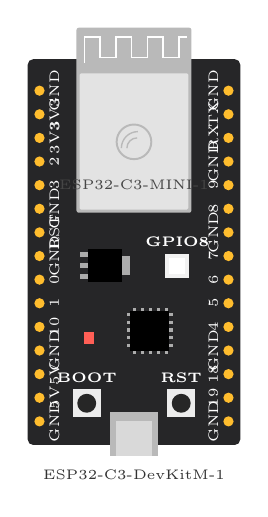
\begin{tikzpicture}
    \pic at (0,0) {esp32c3};
    \node[font=\tiny, text=gray!40!black, anchor=north] at (1.35,-0.2) {ESP32-C3-DevKitM-1};
  \end{tikzpicture}}

% ---------- Wokwi window (schematic; replace with a screenshot if you like) ----------
\newcommand{\wokwiwindow}{%
  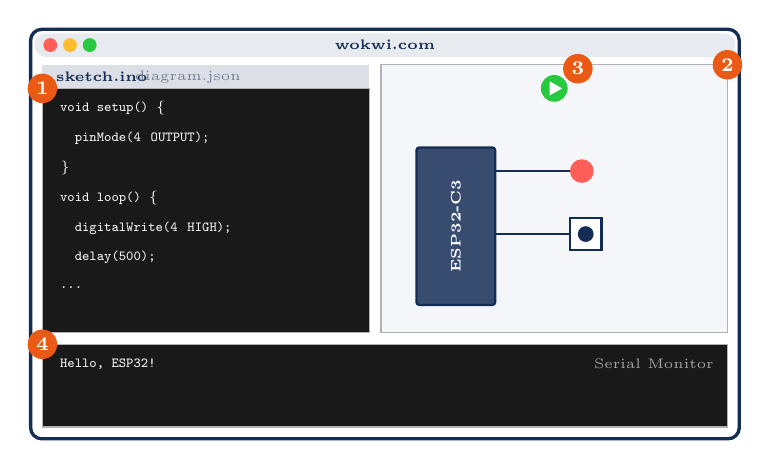
\begin{tikzpicture}[font=\tiny]
    \draw[DeepBlue, very thick, fill=white, rounded corners=4pt] (0,0) rectangle (9,5.2);
    \fill[DeepBlue!10, rounded corners=4pt] (0.05,4.85) rectangle (8.95,5.15);
    \fill[MacRed] (0.25,5.0) circle (2.5pt); \fill[MacYellow] (0.5,5.0) circle (2.5pt); \fill[MacGreen] (0.75,5.0) circle (2.5pt);
    \node[font=\tiny\bfseries, text=DeepBlue] at (4.5,5.0) {wokwi.com};
    % code editor
    \fill[DeepBlue!15] (0.15,4.45) rectangle (4.3,4.75);
    \node[anchor=west, font=\tiny\bfseries, text=DeepBlue] at (0.2,4.6) {sketch.ino};
    \node[anchor=west, font=\tiny, text=DeepBlue!60] at (1.2,4.6) {diagram.json};
    \draw[gray!60, fill=VSDarkBg] (0.15,1.35) rectangle (4.3,4.45);
    \foreach \t [count=\j from 0] in {void setup() \{, \ \ pinMode(4\, OUTPUT);, \}, void loop() \{, \ \ digitalWrite(4\, HIGH);, \ \ delay(500);, \ldots}
      \node[anchor=west, text=VSText, font=\ttfamily\tiny] at (0.25,{4.2-0.38*\j}) {\t};
    % diagram
    \draw[gray!60, fill=LightGray] (4.45,1.35) rectangle (8.85,4.75);
    \fill[MacGreen] (6.65,4.45) circle (0.17);
    \fill[white] (6.59,4.36) -- (6.59,4.54) -- (6.75,4.45) -- cycle;
    \draw[DeepBlue, thick, fill=DeepBlue!85, rounded corners=1pt] (4.9,1.7) rectangle (5.9,3.7);
    \node[font=\tiny\bfseries, text=white, rotate=90] at (5.4,2.7) {ESP32-C3};
    \fill[MacRed] (7.0,3.4) circle (0.15);
    \draw[DeepBlue, thick] (5.9,3.4) -- (6.85,3.4);
    \draw[DeepBlue, thick, fill=white] (6.85,2.4) rectangle (7.25,2.8);
    \fill[DeepBlue] (7.05,2.6) circle (0.1);
    \draw[DeepBlue, thick] (5.9,2.6) -- (6.85,2.6);
    % serial monitor
    \draw[gray!60, fill=VSDarkBg] (0.15,0.15) rectangle (8.85,1.2);
    \node[anchor=west, text=VSText, font=\ttfamily\tiny] at (0.25,0.95) {Hello, ESP32!};
    \node[anchor=east, font=\tiny, text=gray!70] at (8.8,0.95) {Serial Monitor};
    % badges
    \foreach \x/\y/\n in {0.15/4.45/1, 8.85/4.75/2, 6.95/4.7/3, 0.15/1.2/4}
      \node[circle, fill=AccentOrange, text=white, font=\bfseries\scriptsize, inner sep=1.5pt] at (\x,\y) {\n};
  \end{tikzpicture}}

% ---------- our circuit for today ----------
\newcommand{\ourcircuit}{%
  \begin{tikzpicture}[>=Stealth, font=\scriptsize]
    \node[draw=DeepBlue, very thick, fill=DeepBlue!85, text=white, rounded corners=3pt, minimum width=2.0cm,
      minimum height=3.2cm, font=\scriptsize\bfseries, align=center] (esp) at (0,0) {ESP32-C3};
    \node[lbox, draw=MissRed, fill=MissRed!12, minimum width=1.9cm] (led) at (4.2,1.2) {\faLightbulb\ LED};
    \node[lbox, draw=DeepBlue, fill=LightGray, minimum width=1.9cm] (ba) at (4.2,0.4) {\faDotCircle\ Button A};
    \node[lbox, draw=DeepBlue, fill=LightGray, minimum width=1.9cm] (bb) at (4.2,-0.4) {\faDotCircle\ Button B};
    \node[lbox, draw=mygreen, fill=mygreen!12, minimum width=1.9cm] (lcd) at (4.2,-1.25) {\faTv\ LCD 16$\times$2};
    \draw[very thick, DeepBlue] (esp.east |- led) -- node[above, font=\tiny] {GPIO 4} (led);
    \draw[very thick, DeepBlue] (esp.east |- ba) -- node[above, font=\tiny] {GPIO 5} (ba);
    \draw[very thick, DeepBlue] (esp.east |- bb) -- node[above, font=\tiny] {GPIO 6} (bb);
    \draw[very thick, DeepBlue] (esp.east |- lcd) -- node[above, font=\tiny] {GPIO 8, 9 (I2C)} (lcd);
  \end{tikzpicture}}

% ---------- Wokwi-style parts for the "Build it" slides ----------
\definecolor{PcbBlack}{RGB}{38,38,40}
\definecolor{ResBody}{RGB}{214,184,140}
\definecolor{LcdScreen}{RGB}{131,190,40}
\definecolor{WireGreen}{RGB}{0,140,40}
\newcommand{\pinfont}{\fontsize{3.4}{3.6}\selectfont}
\tikzset{
  % a wire; the white edge makes crossings easy to see
  wire/.style={line width=1.1pt, rounded corners=1.5pt, preaction={draw, white, line width=2.6pt}},
  % ESP32-C3-DevKitM-1 as in Wokwi (USB at the bottom); pins (-L0)..(-L14), (-R0)..(-R14), 0 = top
  pics/esp32c3/.style={code={
    \fill[PcbBlack, rounded corners=2pt] (0,0) rectangle (2.7,4.9);
    % module ESP32-C3-MINI-1: the antenna part sticks out above the board
    \fill[gray!55, rounded corners=0.8pt] (0.62,2.95) rectangle (2.08,5.3);
    \draw[white, line width=0.5pt] (0.72,4.85) -- (0.72,5.18)
      \foreach \i in {1,...,3} { -- ++(0.2,0) -- ++(0,-0.26) -- ++(0.2,0) -- ++(0,0.26) } -- ++(0.1,0);
    \fill[gray!22, rounded corners=0.5pt] (0.66,2.99) rectangle (2.04,4.72);
    \draw[gray!55, line width=0.7pt] (1.35,3.85) circle (0.22);
    \draw[gray!55, line width=0.5pt] (1.26,3.77) arc (180:90:0.13) (1.19,3.77) arc (180:90:0.21);
    \node[font=\pinfont, text=gray!55!black] at (1.35,3.3) {ESP32-C3-MINI-1};
    % voltage regulator: 3 small legs on the left, a wide tab on the right
    \foreach \y in {2.14,2.28,2.42} \fill[gray!65] (0.66,\y-0.03) rectangle (0.76,\y+0.03);
    \fill[gray!65] (1.18,2.16) rectangle (1.3,2.4);
    \fill[black] (0.76,2.07) rectangle (1.2,2.49);
    % RGB LED on GPIO 8
    \fill[gray!10] (1.75,2.12) rectangle (2.05,2.42);
    \fill[white] (1.8,2.17) rectangle (2.0,2.37);
    \node[font=\pinfont\bfseries\rmfamily, text=white] at (1.9,2.58) {GPIO8};
    % USB-to-serial chip with pins on all sides
    \foreach \i in {0,...,4} {
      \fill[gray!65] ({1.34+0.1*\i},1.16) rectangle ++(0.04,0.05);
      \fill[gray!65] ({1.34+0.1*\i},1.69) rectangle ++(0.04,0.05);
      \fill[gray!65] (1.26,{1.24+0.1*\i}) rectangle ++(0.05,0.04);
      \fill[gray!65] (1.79,{1.24+0.1*\i}) rectangle ++(0.05,0.04);
    }
    \fill[black] (1.3,1.2) rectangle (1.8,1.7);
    % power LED
    \fill[MacRed] (0.72,1.28) rectangle (0.84,1.44);
    % BOOT and RST buttons
    \foreach \x/\t in {0.75/BOOT,1.95/RST} {
      \fill[gray!15] (\x-0.18,0.35) rectangle (\x+0.18,0.71);
      \fill[black!85] (\x,0.53) circle (0.12);
      \node[font=\pinfont\bfseries\rmfamily, text=white] at (\x,0.86) {\t};
    }
    % USB connector, sticks out below the board
    \fill[gray!55] (1.05,-0.14) rectangle (1.65,0.42);
    \fill[gray!30] (1.12,-0.14) rectangle (1.58,0.3);
    \foreach \n [count=\k from 0] in {GND,3V3,3V3,2,3,GND,RST,GND,0,1,10,GND,5V,5V,GND} {
      \fill[MacYellow] (0.15,{4.5-0.3*\k}) circle (0.065);
      \node[rotate=90, font=\pinfont, text=white] at (0.34,{4.5-0.3*\k}) {\n};
      \coordinate (-L\k) at (0.15,{4.5-0.3*\k});
    }
    \foreach \n [count=\k from 0] in {GND,TX,RX,GND,9,8,GND,7,6,5,4,GND,18,19,GND} {
      \fill[MacYellow] (2.55,{4.5-0.3*\k}) circle (0.065);
      \node[rotate=90, font=\pinfont, text=white] at (2.36,{4.5-0.3*\k}) {\n};
      \coordinate (-R\k) at (2.55,{4.5-0.3*\k});
    }
  }},
  % red LED, origin = middle of the rim; legs (-C) straight, (-A) bent
  pics/wled/.style={code={
    \draw[gray!60, line width=0.9pt] (-0.09,0) -- (-0.09,-0.42);
    \draw[gray!60, line width=0.9pt] (0.09,0) -- (0.09,-0.12) -- (0.17,-0.2) -- (0.17,-0.42);
    \fill[MacRed!80!black] (-0.24,0) rectangle (0.24,0.07);
    \fill[MacRed] (-0.2,0.07) -- (-0.2,0.32) arc (180:0:0.2) -- (0.2,0.07) -- cycle;
    \fill[white, opacity=0.45] (-0.1,0.38) ellipse (0.04 and 0.1);
    \node[font=\pinfont, text=black, anchor=east] at (-0.1,-0.3) {C};
    \node[font=\pinfont, text=black, anchor=west] at (0.18,-0.3) {A};
    \coordinate (-C) at (-0.09,-0.42);
    \coordinate (-A) at (0.17,-0.42);
  }},
  % 220 ohm resistor, vertical; origin = bottom lead (-2), top lead (-1)
  pics/wres/.style={code={
    \draw[gray!60, line width=0.9pt] (0,0) -- (0,0.85);
    \fill[ResBody, rounded corners=0.8pt] (-0.09,0.15) rectangle (0.09,0.7);
    \foreach \y/\c in {0.6/red, 0.52/red, 0.44/brown!80!black, 0.24/MacYellow!70!brown}
      \fill[\c] (-0.09,\y) rectangle (0.09,\y+0.05);
    \coordinate (-1) at (0,0.85);
    \coordinate (-2) at (0,0);
  }},
  % pushbutton, origin = centre; legs (-1l), (-2l), (-1r), (-2r); argument = colour of the cap
  pics/wbutton/.style={code={
    \foreach \x in {-1,1} \foreach \y in {-1,1}
      \draw[gray!60, line width=0.9pt] (0.3*\x,0.13*\y) -- (0.4*\x,0.13*\y);
    \fill[black!80, rounded corners=1pt] (-0.3,-0.25) rectangle (0.3,0.25);
    \fill[gray!35] (-0.25,-0.2) rectangle (0.25,0.2);
    \fill[#1] (0,0) circle (0.14);
    \node[font=\pinfont, text=black, anchor=south east] at (-0.33,0.13) {1.l};
    \node[font=\pinfont, text=black, anchor=north west] at (0.33,-0.13) {2.r};
    \node[font=\pinfont, text=black, anchor=north east] at (-0.33,-0.13) {2.l};
    \node[font=\pinfont, text=black, anchor=south west] at (0.33,0.13) {1.r};
    \coordinate (-1l) at (-0.4,0.13);  \coordinate (-2l) at (-0.4,-0.13);
    \coordinate (-1r) at (0.4,0.13);   \coordinate (-2r) at (0.4,-0.13);
  }},
  % LCD 16x2 with I2C, origin = bottom left; pins (-GND), (-VCC), (-SDA), (-SCL) on the left edge
  pics/wlcd/.style={code={
    \fill[mygreen!55!black, rounded corners=1.5pt] (0,0) rectangle (3.0,1.2);
    \fill[black!85] (0.55,0.12) rectangle (2.9,1.08);
    \fill[LcdScreen] (0.62,0.2) rectangle (2.83,1.0);
    \foreach \r in {0,1} \foreach \c in {0,...,15}
      \fill[LcdScreen!85!black] ({0.66+0.135*\c},{0.26+0.38*\r}) rectangle ++(0.11,0.3);
    \foreach \n [count=\k from 0] in {GND,VCC,SDA,SCL} {
      \fill[MacYellow] (0.14,{1.0-0.2*\k}) circle (0.055);
      \node[font=\pinfont, text=white, anchor=west] at (0.2,{1.0-0.2*\k}) {\n};
      \coordinate (-\n) at (0.14,{1.0-0.2*\k});
    }
  }},
}

% the circuit of the day, built in 4 steps: #1 = step (1 LED, 2 button A, 3 LCD, 4 button B)
% parts of the current step are drawn normally, parts of earlier steps are faded
\newcommand{\buildopacity}[2]{\ifnum#1>#2 0.3\else 1\fi}
\newcommand{\buildpic}[1]{%
  \begin{tikzpicture}[font=\tiny]
    \useasboundingbox (-0.45,-0.2) rectangle (7.3,5.7);
    \pic (esp) at (0,0) {esp32c3};
    % step 1: LED and resistor, GND along the bottom
    \begin{scope}[opacity=\buildopacity{#1}{1}]
      \pic (res) at (4.91,0.65) {wres};
      \pic (led) at (5.0,1.95) {wled};
      \draw[wire, black] (esp-R14) -- (4.91,0.3) -- (res-2);
      \draw[wire, WireGreen] (res-1) -- (led-C);
      \draw[wire, WireGreen] (esp-R10) -| (4.25,0.48) -| (led-A);
      \node[font=\fontsize{5.5}{6}\selectfont\bfseries, anchor=east] at (4.83,1.05) {220\,$\Omega$};
    \end{scope}
    % step 2: button A
    \ifnum#1>1
    \begin{scope}[opacity=\buildopacity{#1}{2}]
      \pic (ba) at (4.9,2.85) {wbutton=MacGreen};
      \node[font=\scriptsize\bfseries, anchor=south] at (4.9,3.1) {A};
      \draw[wire, black] (ba-2r) -| (5.75,0.3) -- (4.91,0.3);
      \draw[wire, WireGreen] (esp-R9) -| ([xshift=-0.35cm]ba-1l) -- (ba-1l);
    \end{scope}
    \fi
    % step 3: LCD (I2C)
    \ifnum#1>2
    \begin{scope}[opacity=\buildopacity{#1}{3}]
      \pic (lcd) at (4.2,4.2) {wlcd};
      \draw[wire, black] (esp-R0) -| ([xshift=-1.09cm]lcd-GND) -- (lcd-GND);
      \draw[wire, StorageBlue] (esp-R5) -| ([xshift=-0.59cm]lcd-SDA) -- (lcd-SDA);
      \draw[wire, ProgramPurple] (esp-R4) -| ([xshift=-0.79cm]lcd-SCL) -- (lcd-SCL);
      \draw[wire, MacRed] (esp-L12) -- (-0.35,0.9) -- (-0.35,5.6) -- (4.0,5.6) |- (lcd-VCC);
    \end{scope}
    \fi
    % step 4: button B
    \ifnum#1>3
    \begin{scope}[opacity=\buildopacity{#1}{4}]
      \pic (bb) at (4.9,3.75) {wbutton=StorageBlue};
      \node[font=\scriptsize\bfseries, anchor=south] at (4.9,4.0) {B};
      \draw[wire, black] (bb-2r) -| (5.75,2.72);
      \fill (5.75,2.72) circle (0.05);
      \draw[wire, WireGreen] (esp-R8) -| ([xshift=-0.55cm]bb-1l) -- (bb-1l);
    \end{scope}
    \fi
  \end{tikzpicture}}

% ---------- power: VCC, GND and a closed loop ----------
\newcommand{\powerexplain}{%
  \begin{tikzpicture}[font=\scriptsize, >=Stealth]
    % rails
    \draw[line width=2pt, MacRed] (0,2.0) -- (4.6,2.0);
    \node[anchor=west, font=\scriptsize\bfseries, text=MacRed, align=left] at (4.7,2.0) {VCC (+)\\[-1pt]{\tiny 3V3 = 3.3\,V, 5V = 5\,V}};
    \draw[line width=2pt, black] (0,-1.0) -- (4.6,-1.0);
    \node[anchor=west, font=\scriptsize\bfseries, align=left] at (4.7,-1.0) {GND ($-$)\\[-1pt]{\tiny 0\,V}};
    % voltage between the rails
    \draw[<->, thick, DeepBlue] (-0.4,-1.0) -- node[left, font=\scriptsize\bfseries, align=center] {voltage\\3.3\,V} (-0.4,2.0);
    % a part between the rails: resistor + LED
    \draw[thick] (1.2,2.0) -- (1.2,1.55);
    \draw[thick, fill=ResBody] (1.08,1.55) rectangle (1.32,0.85);
    \draw[thick] (1.2,0.85) -- (1.2,0.6);
    \draw[thick, fill=MacRed!35] (0.95,0.6) -- (1.45,0.6) -- (1.2,0.15) -- cycle;
    \draw[very thick] (0.95,0.15) -- (1.45,0.15);
    \foreach \d in {0,0.15} \draw[->, MacRed, thick] (1.5,{0.45-\d}) -- ++(0.28,0.16);
    \draw[thick] (1.2,0.15) -- (1.2,-1.0);
    \fill[MacRed] (1.2,2.0) circle (0.06);  \fill (1.2,-1.0) circle (0.06);
    \draw[->, line width=1.4pt, AccentOrange] (0.65,1.8) -- node[sloped, above, font=\tiny\bfseries] {current} (0.65,-0.8);
    \node[font=\tiny\bfseries, mygreen, align=center] at (1.2,-1.4) {\faCheck\ closed loop:\\+ $\to$ part $\to$ GND};
    % a short circuit
    \draw[line width=1.4pt, MacRed] (3.6,2.0) -- (3.6,-1.0);
    \fill[MacRed] (3.6,2.0) circle (0.06);  \fill (3.6,-1.0) circle (0.06);
    \node[font=\Large\bfseries, text=MacRed, fill=white, inner sep=1pt] at (3.6,0.5) {\faTimes};
    \node[font=\tiny\bfseries, MacRed, align=center] at (3.6,-1.4) {\faTimes\ short circuit:\\VCC straight to GND};
  \end{tikzpicture}}

% ---------- how an LED works: the part and its circuit ----------
\newcommand{\ledexplain}{%
  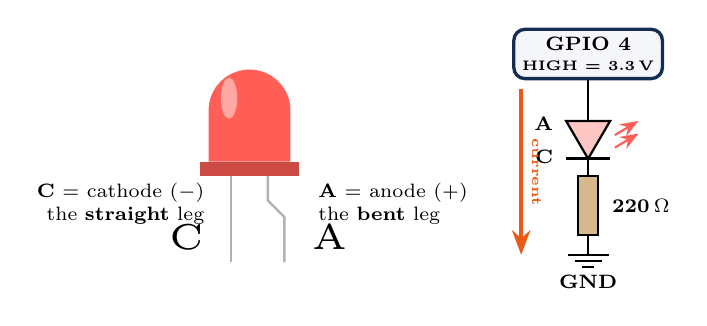
\begin{tikzpicture}[font=\scriptsize, >=Stealth]
    \begin{scope}[scale=2.6, transform shape]
      \pic (bl) at (0,0) {wled};
    \end{scope}
    \node[anchor=west, align=left] (la) at (0.75,-0.35) {\textbf{A} = anode (+)\\the \textbf{bent} leg};
    \node[anchor=east, align=right] (lc) at (-0.45,-0.35) {\textbf{C} = cathode ($-$)\\the \textbf{straight} leg};
    % the circuit
    \begin{scope}[xshift=4.3cm, yshift=-0.2cm]
      \node[lbox, draw=DeepBlue, fill=LightGray] (gpio) at (0,1.75) {GPIO 4\\[-1pt]{\tiny HIGH = 3.3\,V}};
      \draw[thick] (gpio.south) -- (0,0.9);
      \draw[thick, fill=MacRed!35] (-0.28,0.9) -- (0.28,0.9) -- (0,0.42) -- cycle;
      \draw[very thick] (-0.28,0.42) -- (0.28,0.42);
      \foreach \d in {0,0.16} \draw[->, MacRed, thick] (0.34,{0.72-\d}) -- ++(0.3,0.18);
      \node[anchor=east, font=\scriptsize\bfseries] at (-0.32,0.86) {A};
      \node[anchor=east, font=\scriptsize\bfseries] at (-0.32,0.44) {C};
      \draw[thick] (0,0.42) -- (0,0.2);
      \draw[thick, fill=ResBody] (-0.13,0.2) rectangle (0.13,-0.55);
      \node[anchor=west, font=\scriptsize\bfseries] at (0.18,-0.18) {220\,$\Omega$};
      \draw[thick] (0,-0.55) -- (0,-0.8);
      \foreach \w/\y in {0.26/-0.8, 0.17/-0.88, 0.08/-0.96} \draw[thick] (-\w,\y) -- (\w,\y);
      \node[font=\scriptsize\bfseries] at (0,-1.15) {GND};
      \draw[->, line width=1.3pt, AccentOrange] (-0.85,1.3) -- node[sloped, above, font=\tiny\bfseries] {current} (-0.85,-0.8);
    \end{scope}
  \end{tikzpicture}}

% ---------- how a pushbutton works: 4 legs, 2 pairs ----------
% #1 = 0 not pressed, 1 pressed
\newcommand{\buttoninside}[1]{%
  \begin{tikzpicture}[font=\tiny, >=Stealth]
    \foreach \x/\y/\n in {0/0.8/1.l, 1.6/0.8/1.r, 0/0/2.l, 1.6/0/2.r} {
      \fill[gray!60] (\x,\y) circle (0.06);
      \node[font=\tiny\bfseries, anchor=\ifdim\x pt<1pt east\else west\fi] at (\x,\y) {\n};
    }
    \draw[thick] (0,0.8) -- (1.6,0.8);
    \draw[thick] (0,0) -- (1.6,0);
    \fill (0.8,0.8) circle (0.04);  \fill (0.8,0) circle (0.04);
    \ifnum#1=0
      \draw[thick] (0.8,0.8) -- (0.8,0.62) -- (1.1,0.22);
      \draw[thick] (0.8,0) -- (0.8,0.18);
    \else
      \draw[line width=1.6pt, mygreen] (0.8,0.8) -- (0.8,0);
    \fi
  \end{tikzpicture}}
\newcommand{\buttonexplain}{%
  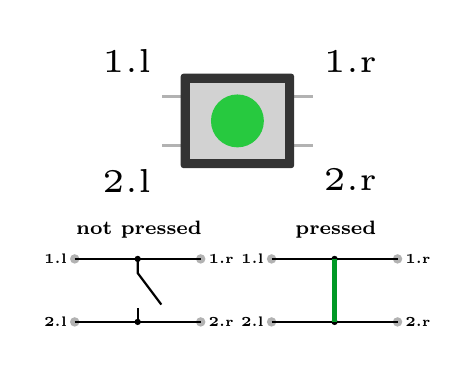
\begin{tikzpicture}[font=\scriptsize]
    \begin{scope}[scale=2.4, transform shape]
      \pic (bx) at (0,0) {wbutton=MacGreen};
    \end{scope}
    \node[anchor=north, align=center] at (-1.25,-1.15) {\textbf{not pressed}\\[2pt]\buttoninside{0}};
    \node[anchor=north, align=center] at (1.25,-1.15) {\textbf{pressed}\\[2pt]\buttoninside{1}};
  \end{tikzpicture}}

% ---------- I2C: one controller, many devices on 2 wires ----------
\newcommand{\itwocbus}{%
  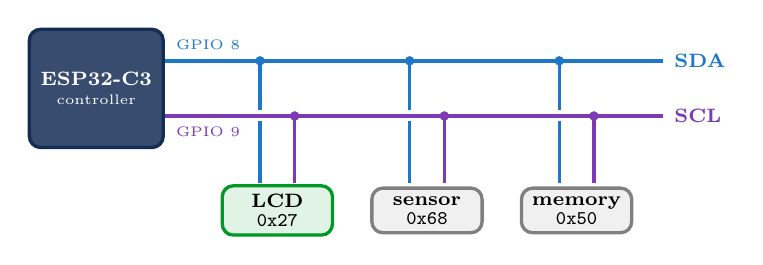
\begin{tikzpicture}[font=\scriptsize, >=Stealth]
    \node[lbox, draw=DeepBlue, fill=DeepBlue!85, text=white, minimum width=1.7cm, minimum height=1.5cm]
      (cpu) at (0,0) {ESP32-C3\\[-1pt]{\tiny\mdseries controller}};
    \draw[line width=1.5pt, StorageBlue] (cpu.east |- 0,0.35) node[above right, font=\tiny] {GPIO 8} -- (7.2,0.35)
      node[right, font=\scriptsize\bfseries] {SDA};
    \foreach \x/\n/\a/\c in {2.3/LCD/0x27/mygreen, 4.2/sensor/0x68/gray, 6.1/memory/0x50/gray} {
      \draw[line width=1.2pt, StorageBlue] (\x-0.22,0.35) -- (\x-0.22,-1.2);
      \fill[StorageBlue] (\x-0.22,0.35) circle (0.06);
      \node[lbox, draw=\c, fill=\c!12, minimum width=1.4cm] at (\x,-1.55) {\n\\[-1pt]\texttt{\a}};
    }
    \draw[line width=1.5pt, ProgramPurple, preaction={draw, white, line width=4pt}] (cpu.east |- 0,-0.35)
      node[below right, font=\tiny] {GPIO 9} -- (7.2,-0.35) node[right, font=\scriptsize\bfseries] {SCL};
    \foreach \x in {2.3,4.2,6.1} {
      \draw[line width=1.2pt, ProgramPurple] (\x+0.22,-0.35) -- (\x+0.22,-1.2);
      \fill[ProgramPurple] (\x+0.22,-0.35) circle (0.06);
    }
  \end{tikzpicture}}

% ---------- one I2C message on the wires: #1 = the step to highlight (1..6) ----------
\newcommand{\itwoctiming}[1]{%
  \begin{tikzpicture}[font=\scriptsize, >=Stealth]
    % the steps: highlighted band and a label on top
    \foreach \n/\a/\b/\t/\c in {1/0.3/1.0/START/AccentOrange, 2/1.0/5.0/{address \texttt{0x27} + write}/StorageBlue,
        3/5.0/5.5/ACK/mygreen, 4/5.5/9.5/{data byte}/StorageBlue, 5/9.5/10.0/ACK/mygreen, 6/10.0/10.75/STOP/AccentOrange} {
      \ifnum\n=#1
        \fill[\c!18, rounded corners=2pt] (\a,-1.55) rectangle (\b,1.45);
        \node[font=\scriptsize\bfseries, text=\c!80!black] at ({(\a+\b)/2},1.25) {\t};
      \else
        \node[font=\tiny, text=gray] at ({(\a+\b)/2},1.25) {\t};
      \fi
      \draw[gray!40, densely dotted] (\a,-1.55) -- (\a,1.1);
    }
    \node[anchor=east, font=\scriptsize\bfseries, text=ProgramPurple] at (-0.1,0.6) {SCL};
    \node[anchor=east, font=\scriptsize\bfseries, text=StorageBlue] at (-0.1,-0.6) {SDA};
    % SCL: high, falls after START, 18 clock ticks, high again before STOP
    \draw[thick, ProgramPurple] (0,0.9) -- (0.8,0.9) -- (0.8,0.3) -- (1.25,0.3)
      \foreach \k in {0,...,17} { -- ({1.25+0.5*\k},0.9) -- ({1.5+0.5*\k},0.9) -- ({1.5+0.5*\k},0.3) -- ({1.75+0.5*\k},0.3) }
      -- (10.2,0.3) -- (10.2,0.9) -- (10.9,0.9);
    % SDA: falls at START, one bit per tick, rises at STOP
    \draw[thick, StorageBlue] (0,-0.3) -- (0.5,-0.3) -- (0.5,-0.9) -- (1.0,-0.9);
    \foreach \x/\p/\v/\c in {1.0/0/0/StorageBlue, 1.5/0/1/StorageBlue, 2.0/1/0/StorageBlue, 2.5/0/0/StorageBlue, 3.0/0/1/StorageBlue, 3.5/1/1/StorageBlue, 4.0/1/1/StorageBlue, 4.5/1/0/StorageBlue, 5.0/0/0/mygreen, 5.5/0/0/StorageBlue, 6.0/0/1/StorageBlue, 6.5/1/0/StorageBlue, 7.0/0/0/StorageBlue, 7.5/0/1/StorageBlue, 8.0/1/0/StorageBlue, 8.5/0/0/StorageBlue, 9.0/0/0/StorageBlue, 9.5/0/0/mygreen}
      \draw[thick, \c] (\x,{-0.9+0.6*\p}) -- (\x,{-0.9+0.6*\v}) -- (\x+0.5,{-0.9+0.6*\v});
    \draw[thick, StorageBlue] (10.0,-0.9) -- (10.45,-0.9) -- (10.45,-0.3) -- (10.9,-0.3);
    \foreach \x/\v in {1.25/0, 1.75/1, 2.25/0, 2.75/0, 3.25/1, 3.75/1, 4.25/1, 4.75/0, 5.25/0, 5.75/0, 6.25/1, 6.75/0, 7.25/0, 7.75/1, 8.25/0, 8.75/0, 9.25/0, 9.75/0} \node[font=\tiny, text=gray!70!black] at (\x,-1.2) {\v};
    \node[font=\tiny, text=gray!70!black] at (4.75,-1.42) {W};
  \end{tikzpicture}}

% ---------- showcase: Snake on a Nokia 5110 screen with a joystick ----------
\newcommand{\snakeshowcase}{%
  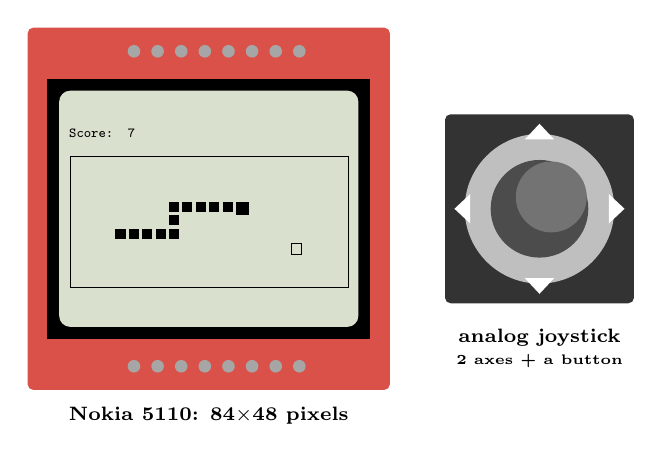
\begin{tikzpicture}[font=\scriptsize]
    % the Nokia 5110 module
    \fill[MacRed!85!black, rounded corners=2pt] (0,0) rectangle (4.6,4.6);
    \foreach \i in {0,...,7} {
      \fill[gray!70] ({1.35+0.3*\i},0.3) circle (0.08);
      \fill[gray!70] ({1.35+0.3*\i},4.3) circle (0.08);
    }
    \fill[black] (0.25,0.65) rectangle (4.35,3.95);
    \fill[LcdScreen!40!gray!30, rounded corners=4pt] (0.4,0.8) rectangle (4.2,3.8);
    % the game: 84 x 48 pixels drawn at 0.0425 cm per pixel
    \begin{scope}[shift={(0.52,3.32)}, x=0.0425cm, y=-0.0425cm]
      \node[anchor=north west, inner sep=0, font=\ttfamily\bfseries\tiny] at (0,0) {Score: 7};
      \draw[line width=0.3pt] (0.5,8.5) rectangle (83.5,47.5);
      \foreach \x/\y in {3/5,4/5,5/5,6/5,7/5,7/4,7/3,8/3,9/3,10/3,11/3} \fill ({2+4*\x},{10+4*\y}) rectangle ++(3,3);
      \fill ({2+4*12},{10+4*3}) rectangle ++(4,4);
      \draw[line width=0.3pt] ({2+4*16+0.5},{10+4*6+0.5}) rectangle ++(3,3);
    \end{scope}
    \node[font=\scriptsize\bfseries, anchor=north] at (2.3,-0.1) {Nokia 5110: 84$\times$48 pixels};
    % the joystick
    \begin{scope}[shift={(5.3,1.1)}]
      \fill[black!80, rounded corners=2pt] (0,0) rectangle (2.4,2.4);
      \fill[gray!50] (1.2,1.2) circle (0.95);
      \fill[black!70] (1.2,1.2) circle (0.62);
      \fill[black!55] (1.35,1.35) circle (0.45);
      \foreach \a in {0,90,180,270} \fill[white] ([shift={(\a:1.08)}]1.2,1.2) -- ([shift={(\a+12:0.9)}]1.2,1.2) -- ([shift={(\a-12:0.9)}]1.2,1.2) -- cycle;
      \node[font=\scriptsize\bfseries, anchor=north, align=center] at (1.2,-0.2) {analog joystick\\{\tiny 2 axes + a button}};
    \end{scope}
  \end{tikzpicture}}

% ---------- inside the ESP32-C3: CPU, internal bus, controllers; pins and wires outside ----------
% #1 = 0 overview, 1 address on the bus, 2 GPIO recognises it, 3 data written: the LED lights up
\newcommand{\chipbus}[1]{%
  \begin{tikzpicture}[>=Stealth, font=\scriptsize]
    % the chip
    \draw[DeepBlue, very thick, dashed, rounded corners=6pt, fill=DeepBlue!4] (-1.3,-1.6) rectangle (11.9,2.5);
    \node[anchor=north west, font=\scriptsize\bfseries, text=DeepBlue] at (-1.2,2.45) {\faMicrochip\ inside the ESP32-C3 chip};
    \node[cpubox, minimum width=1.8cm, minimum height=0.9cm] (cpu) at (0.4,1.45) {CPU};
    % the internal bus
    \ifnum#1>0 \def\buswidth{1.5pt}\else \def\buswidth{2pt}\fi
    \foreach \y/\c/\t in {0.75/AccentOrange/address, 0.45/StorageBlue/data, 0.15/ProgramPurple/control} {
      \draw[line width=\buswidth, \c] (0.4,\y) -- (10.4,\y);
      \node[anchor=west, font=\tiny\bfseries, text=\c] at (10.45,\y) {\t};
    }
    \node[font=\tiny\bfseries, text=DeepBlue, anchor=south] at (5.4,0.78) {internal bus};
    \draw[very thick, DeepBlue] (cpu.south) -- (0.4,0.15);
    % memory and controllers
    \node[rambox, minimum width=2.0cm, minimum height=0.85cm] (mem) at (2.9,-0.75) {Memory\\[-1pt]{\tiny\mdseries RAM, flash}};
    \node[iobox, minimum width=2.0cm, minimum height=0.85cm] (gpio) at (6.0,-0.75) {GPIO controller\\[-1pt]{\tiny\mdseries \texttt{0x6000\,4000}}};
    \node[iobox, minimum width=2.0cm, minimum height=0.85cm] (i2c) at (9.1,-0.75) {I2C controller\\[-1pt]{\tiny\mdseries \texttt{0x6001\,3000}}};
    \foreach \n in {mem,gpio,i2c} \draw[very thick, DeepBlue] (\n.north) -- (\n.north |- 0,0.75);
    % every connection reaches all three groups of lines: address, data and control
    \foreach \x in {0.4,2.9,6.0,9.1}
      \foreach \y/\c in {0.75/AccentOrange, 0.45/StorageBlue, 0.15/ProgramPurple}
        \fill[\c] (\x,\y) circle (0.075);
    % pins on the edge of the chip, wires on the board
    \foreach \x/\l/\n in {5.6/4/gpio, 6.4/5/gpio, 8.7/8/i2c, 9.5/9/i2c} {
      \draw[thick, gray!70!black] (\x,-1.175) -- (\x,-1.6);
      \fill[MacYellow] (\x-0.09,-1.69) rectangle (\x+0.09,-1.51);
      \node[font=\tiny\bfseries, anchor=west] at (\x+0.08,-1.4) {\l};
    }
    \draw[line width=1.2pt, WireGreen] (5.6,-1.69) -- (5.6,-2.25);
    \draw[line width=1.2pt, WireGreen] (6.4,-1.69) -- (6.4,-2.25);
    \draw[line width=1.2pt, StorageBlue] (8.7,-1.69) -- (8.7,-2.2);
    \draw[line width=1.2pt, ProgramPurple] (9.5,-1.69) -- (9.5,-2.2);
    \ifnum#1=3
      \fill[MacRed!30] (5.6,-2.5) circle (0.38);
      \fill[MacRed] (5.6,-2.5) circle (0.24);
      \node[font=\tiny\bfseries, text=MacRed, anchor=east] at (5.5,-1.95) {3.3\,V};
    \else
      \fill[MacRed!35] (5.6,-2.5) circle (0.24);
    \fi
    \node[font=\tiny, anchor=north] at (5.6,-2.78) {LED};
    \fill[black!75, rounded corners=1pt] (6.2,-2.7) rectangle (6.6,-2.3);  \fill[MacGreen] (6.4,-2.5) circle (0.12);
    \node[font=\tiny, anchor=north] at (6.4,-2.78) {button};
    \node[lbox, draw=mygreen, fill=mygreen!12, minimum width=1.6cm] (lcd) at (9.1,-2.55) {LCD\\[-1pt]{\tiny\mdseries I2C address \texttt{0x27}}};
    \node[font=\tiny, text=gray!40!black, anchor=west, align=left] at (10.05,-1.95) {SDA, SCL:\\2 wires};
    \node[font=\scriptsize\bfseries, text=gray!40!black, anchor=west] at (-1.2,-2.2) {on the board: real wires};
    % the steps of one store: sw to 0x6000 4008
    \ifnum#1>0
      \node[font=\tiny\ttfamily, fill=white, draw=DeepBlue, rounded corners=1pt, anchor=west] at (1.5,1.45) {sw a4, 8(a5)};
      \node[font=\tiny\bfseries\ttfamily, fill=AccentOrange!20, draw=AccentOrange, rounded corners=1pt] at (1.8,0.75) {0x6000\,4008};
    \fi
    \ifnum#1>1
      \draw[line width=1.6pt, mygreen, rounded corners=3pt] ([shift={(-0.08,-0.08)}]gpio.south west) rectangle ([shift={(0.08,0.08)}]gpio.north east);
      \node[font=\tiny\bfseries, text=mygreen, anchor=south west] at ([xshift=0.05cm]gpio.north east) {mine!};
      \node[font=\tiny, text=gray, anchor=south west] at ([xshift=0.05cm]mem.north east) {not mine};
      \node[font=\tiny, text=gray, anchor=south west] at ([xshift=0.05cm]i2c.north east) {not mine};
    \fi
    \ifnum#1>2
      \node[font=\tiny\bfseries\ttfamily, fill=StorageBlue!20, draw=StorageBlue, rounded corners=1pt] at (1.8,0.45) {0x10 = bit 4};
      \node[font=\tiny\bfseries, fill=ProgramPurple!15, draw=ProgramPurple, rounded corners=1pt] at (1.8,0.15) {write};
    \fi
  \end{tikzpicture}}

% ---------- lcd.print: CPU -> I2C controller (internal bus) -> LCD (2 wires) ----------
\newcommand{\twobuses}{%
  \begin{tikzpicture}[>=Stealth, font=\scriptsize]
    \draw[DeepBlue, very thick, dashed, rounded corners=6pt, fill=DeepBlue!4] (-0.3,-0.75) rectangle (5.3,1.2);
    \node[anchor=north west, font=\tiny\bfseries, text=DeepBlue] at (-0.25,1.17) {\faMicrochip\ inside the chip};
    \node[cpubox, minimum width=1.4cm, minimum height=0.8cm] (cpu) at (0.6,0.1) {CPU};
    \node[iobox, minimum width=1.8cm, minimum height=0.8cm] (ctl) at (4.1,0.1) {I2C\\[-1pt]controller};
    \draw[->, line width=1.8pt, AccentOrange] (cpu.east) -- node[above, font=\tiny\bfseries] {internal bus} node[below, font=\tiny\ttfamily] {sw \ldots\ 0x6001\,3xxx} (ctl.west);
    \node[lbox, draw=mygreen, fill=mygreen!12, minimum width=1.4cm, minimum height=0.8cm] (lcd) at (7.3,0.1) {LCD\\[-1pt]{\tiny\mdseries \texttt{0x27}}};
    \draw[->, line width=1.2pt, StorageBlue] ([yshift=0.12cm]ctl.east) -- ([yshift=0.12cm]lcd.west);
    \draw[line width=1.2pt, ProgramPurple] ([yshift=-0.12cm]ctl.east) -- ([yshift=-0.12cm]lcd.west);
    \node[font=\tiny\bfseries, anchor=south] at (6.05,0.25) {SDA, SCL};
    \node[font=\tiny, anchor=north, align=center] at (6.05,-0.05) {START, \texttt{0x27},\\data, STOP};
    \node[font=\tiny\bfseries, text=gray!40!black] at (6.05,-0.95) {on the board};
    \node[font=\tiny\ttfamily, anchor=north] at (0.6,-0.32) {lcd.print("K")};
  \end{tikzpicture}}

% ---------- memory-mapped I/O: one address space, the device part zoomed in ----------
\newcommand{\mmiomap}{%
  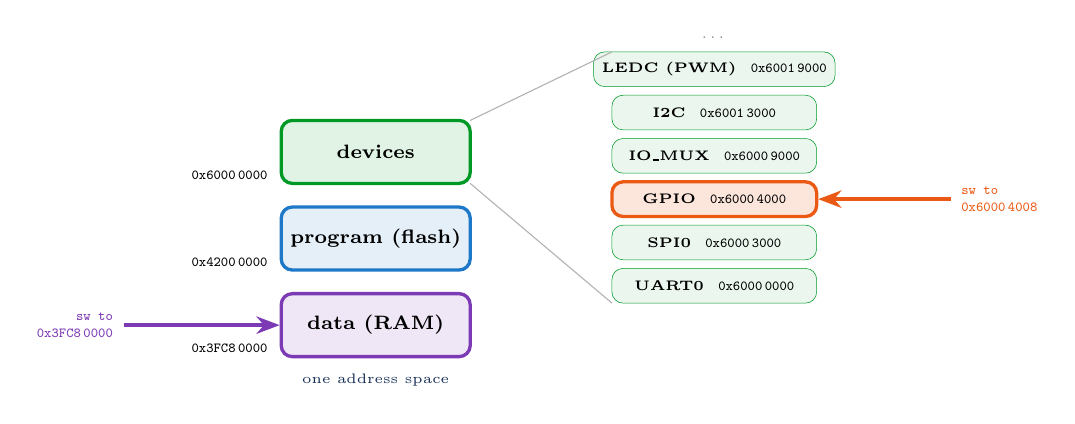
\begin{tikzpicture}[>=Stealth, font=\scriptsize]
    \foreach \y/\n/\a/\c in {2.3/devices/0x6000\,0000/cIO, 1.2/program (flash)/0x4200\,0000/cRAM, 0.1/data (RAM)/0x3FC8\,0000/cCache} {
      \node[lbox, draw=\c, fill=\c!12, minimum width=2.4cm, minimum height=0.8cm] (\n) at (0,\y) {\n};
      \node[font=\ttfamily\tiny, anchor=east] at (-1.25,\y-0.3) {\a};
    }
    \node[font=\tiny, text=DeepBlue, anchor=north] at (0,-0.4) {one address space};
    % the device part, zoomed in: one window per controller
    \foreach \y/\n/\a/\h in {3.35/LEDC (PWM)/0x6001\,9000/0, 2.8/I2C/0x6001\,3000/0, 2.25/IO\_MUX/0x6000\,9000/0,
                             1.7/GPIO/0x6000\,4000/1, 1.15/SPI0/0x6000\,3000/0, 0.6/UART0/0x6000\,0000/0} {
      \ifnum\h=1
        \node[lbox, draw=AccentOrange, fill=AccentOrange!15, minimum width=2.6cm, minimum height=0.44cm, font=\tiny\bfseries] at (4.3,\y) {\n\ \ \texttt{\mdseries\a}};
      \else
        \node[lbox, draw=cIO, fill=cIO!8, minimum width=2.6cm, minimum height=0.44cm, font=\tiny\bfseries, very thin] at (4.3,\y) {\n\ \ \texttt{\mdseries\a}};
      \fi
    }
    \draw[gray!60, thin] (1.2,2.7) -- (3.0,3.57);
    \draw[gray!60, thin] (1.2,1.9) -- (3.0,0.38);
    \node[font=\tiny, text=gray] at (4.3,3.75) {\ldots};
    % two stores
    \draw[->, very thick, AccentOrange] (7.3,1.7) node[right, font=\tiny\bfseries\ttfamily, align=left] {sw to\\0x6000\,4008} -- (5.62,1.7);
    \draw[->, very thick, cCache] (-3.2,0.1) node[left, font=\tiny\bfseries\ttfamily, align=right] {sw to\\0x3FC8\,0000} -- (-1.22,0.1);
  \end{tikzpicture}}

% ---------- small arrow "program flow" pieces ----------
\tikzset{
  instr/.style={draw=DeepBlue!60, fill=white, minimum width=1.9cm, minimum height=0.38cm, inner sep=1pt,
    font=\ttfamily\tiny},
  isrinstr/.style={instr, draw=cISR, fill=cISR!15},
}

% =====================================================================
%  Day 6 helpers
% =====================================================================

% ---------- names that may still change: Wokwi projects and the simulator ----------
\newcommand{\projCircuit}{\textbf{Circuit}}       % the circuit from Lecture 5
\newcommand{\projLeds}{\textbf{Three LEDs}}       % the circuit with LEDs on GPIO 4, 7 and 3
\newcommand{\projRace}{\textbf{Race}}             % starter code for Task 5
\newcommand{\simname}{\textbf{ConcurrencySimulator}}
\newcommand{\simurl}{\texttt{ksawerym.github.io/ConcurrencySimulator}}
% a topic (tab) of the simulator
\newcommand{\simtab}[1]{\textcolor{ProgramPurple}{\textbf{#1}}}

% ---------- colours used all day ----------
\colorlet{cTaskA}{StorageBlue}
\colorlet{cTaskB}{ProgramPurple}
\colorlet{cTaskC}{mygreen}
\colorlet{cTaskH}{MacRed}
\colorlet{cSched}{AccentOrange}
\colorlet{cLed}{MacRed}

% ---------- listings ----------
% C++ in Wokwi with the FreeRTOS functions
\lstdefinestyle{rtos}{style=ino,
  morekeywords={TickType_t},
  emph={pinMode,digitalWrite,digitalRead,delay,millis,attachInterrupt,digitalPinToInterrupt,
    timerBegin,timerAttachInterrupt,timerAlarm,xTaskCreate,vTaskDelay,vTaskDelayUntil,vTaskDelete,
    pdMS_TO_TICKS,pcTaskGetName,uxTaskPriorityGet,xTaskGetTickCount}}
% FreeRTOS source code (C)
\lstdefinestyle{frc}{style=cc, morekeywords={StackType_t,ListItem_t,UBaseType_t,TCB_t}}
% RISC-V with the instructions used today
\lstdefinestyle{rv6}{style=rv, morekeywords={j,mret,csrr,csrw}}

% ---------- an interrupt on a timeline ----------
\newcommand{\irqtimeline}{%
  \begin{tikzpicture}[>=Stealth, font=\scriptsize]
    \node[anchor=east, font=\scriptsize\bfseries, text=DeepBlue] at (-0.15,0) {main program};
    \node[anchor=east, font=\scriptsize\bfseries, text=cISR] at (-0.15,-1.0) {ISR};
    \fill[cWork] (0,-0.21) rectangle (3.6,0.21);
    \fill[cWork] (4.8,-0.21) rectangle (9.2,0.21);
    \node[font=\tiny\bfseries, text=white] at (1.8,0) {main program};
    \node[font=\tiny\bfseries, text=white] at (7.0,0) {main program continues};
    \draw[cWork, thick, dashed] (3.6,0) -- (4.8,0);
    \fill[cISR] (3.6,-1.21) rectangle (4.8,-0.79);
    \node[font=\tiny\bfseries, text=white] at (4.2,-1.0) {ISR};
    \draw[->, very thick, DeepBlue] (3.6,-0.25) -- (3.6,-0.75);
    \draw[->, very thick, DeepBlue] (4.8,-0.75) -- (4.8,-0.25);
    \node[anchor=east, font=\scriptsize] at (3.5,-0.5) {\badge{1}\ suspend};
    \node[font=\scriptsize, anchor=north] at (4.2,-1.3) {\badge{2}\ run the ISR};
    \node[anchor=west, font=\scriptsize] at (4.9,-0.5) {\badge{3}\ return};
    % the signal from the button
    \node[font=\Large, text=cIO] at (3.6,1.45) {\faDotCircle};
    \node[anchor=west, font=\scriptsize\bfseries, text=cIO] at (3.95,1.45) {button A is pressed};
    \draw[->, very thick, cIO] (3.6,1.15) -- (3.6,0.3);
    \draw[->, thick, DeepBlue] (0,-1.95) -- (9.4,-1.95) node[right, font=\tiny] {time};
  \end{tikzpicture}}

% ---------- inside the processor: one interrupt in 4 steps ----------
% #1 = step (1 signal, 2 save and jump, 3 the ISR runs, 4 return)
\newcommand{\irqsteps}[1]{%
  \begin{tikzpicture}[>=Stealth, font=\scriptsize,
      hotinstr/.style={instr, fill=AccentOrange!35, draw=AccentOrange, very thick}]
    \useasboundingbox (-1.75,-1.1) rectangle (7.65,2.65);
    % the main program
    \node[font=\scriptsize\bfseries, text=DeepBlue] at (1.6,2.4) {main program};
    \foreach \a/\t [count=\k from 0] in {0x0100/{li\ \ \ t0, 0}, 0x0104/{addi t0, t0, 1},
        0x0108/{sw\ \ \ t0, 0(a0)}, 0x010C/{j\ \ \ \ 0x0104}} {
      \node[addr, font=\ttfamily\tiny, anchor=east] at (0.45,{1.95-0.45*\k}) {\a};
      \node[instr, minimum width=2.2cm] (m\k) at (1.6,{1.95-0.45*\k}) {\t};
    }
    % the ISR
    \node[font=\scriptsize\bfseries, text=cISR] at (5.75,2.4) {ISR: \texttt{onButtonA}};
    \foreach \a/\t [count=\k from 0] in {0x0200/{save t0}, 0x0204/{presses++}, 0x0208/{restore t0},
        0x020C/{return}} {
      \node[addr, font=\ttfamily\tiny, anchor=west] at (6.9,{1.95-0.45*\k}) {\a};
      \node[isrinstr, minimum width=2.2cm] (i\k) at (5.75,{1.95-0.45*\k}) {\t};
    }
    % highlighted instructions
    \ifnum#1=1 \node[hotinstr, minimum width=2.2cm] at (m1) {addi t0, t0, 1}; \fi
    \ifnum#1=3
      \foreach \k in {0,...,3} \draw[cISR, line width=1.6pt] (i\k.south west) rectangle (i\k.north east);
    \fi
    \ifnum#1=4 \node[hotinstr, minimum width=2.2cm] at (m2) {sw\ \ \ t0, 0(a0)}; \fi
    % the signal
    \ifnum#1=1
      \node[font=\scriptsize\bfseries, text=cIO, align=center] (sig) at (-1.05,1.5) {\faDotCircle\\interrupt!};
      \draw[->, very thick, cIO] (sig.east) -- ([xshift=-0.75cm]m1.west);
    \fi
    % jump and return
    \ifnum#1=2 \draw[->, very thick, DeepBlue] (m1.east) to[out=0, in=180] node[pos=0.3, above, font=\tiny\bfseries] {jump} (i0.west); \fi
    \ifnum#1=4 \draw[->, very thick, DeepBlue] (i3.west) to[out=180, in=0] node[pos=0.75, below, font=\tiny\bfseries] {return} (m2.east); \fi
    % registers
    \ifcase#1 \or \def\pcv{0x0104}\def\spcv{--}%
      \or \def\pcv{0x0200}\def\spcv{0x0108}%
      \or \def\pcv{0x0204}\def\spcv{0x0108}%
      \or \def\pcv{0x0108}\def\spcv{0x0108}\fi
    \node[reg, minimum width=2.2cm] (pc) at (1.6,-0.55) {\textbf{PC}\ \ \pcv};
    \node[reg, minimum width=2.2cm, fill=gray!10, draw=gray] (spc) at (5.75,-0.55) {\textbf{saved PC}\ \ \spcv};
    \ifnum#1=2 \draw[WriteRed, line width=1.6pt, rounded corners=2pt] (spc.south west) rectangle (spc.north east); \fi
    \ifnum#1=4
      \draw[ReadBlue, line width=1.6pt, rounded corners=2pt] (spc.south west) rectangle (spc.north east);
      \draw[->, very thick, DeepBlue] (spc.west) -- (pc.east);
    \fi
  \end{tikzpicture}}

% ---------- the button with an interrupt (figure 1 of the course plan) ----------
\newcommand{\figbuttonisr}{%
  \begin{tikzpicture}[>=Stealth, font=\scriptsize]
    \draw[DeepBlue, very thick, rounded corners=6pt, fill=DeepBlue!5] (0,-0.3) rectangle (4.8,2.75);
    \node[anchor=north west, font=\scriptsize\bfseries, text=DeepBlue] at (0.1,2.7) {\faMicrochip\ ESP32-C3};
    \node[lbox, draw=cISR, fill=cISR!15, minimum width=4.1cm, minimum height=0.85cm] (isr) at (2.4,1.6)
      {interrupt handler (ISR)\\[-1pt]{\ttfamily\mdseries presses++}};
    \node[lbox, draw=cWork, fill=cWork!12, minimum width=4.1cm, minimum height=0.85cm] (main) at (2.4,0.3)
      {main program\\[-1pt]{\mdseries does not check the button}};
    \draw[->, thick, dashed, DeepBlue] (isr.south) -- node[right, font=\tiny] {\texttt{presses}} (main.north);
    \node[lbox, draw=DeepBlue, fill=LightGray, minimum width=2.0cm] (btn) at (-2.3,1.6)
      {\faDotCircle\ Button A\\[-1pt]{\tiny\mdseries GPIO 5}};
    \draw[->, very thick, cISR] (btn.east) -- node[above, font=\tiny\bfseries] {interrupt} (isr.west);
    \node[draw=mygreen!60!black, fill=mygreen!55!black, rounded corners=2pt, minimum width=2.5cm,
      minimum height=0.8cm] (lcd) at (7.9,0.3) {};
    \node[fill=LcdScreen!45, minimum width=2.2cm, minimum height=0.5cm, font=\ttfamily\scriptsize] at (lcd) {Presses: 3};
    \node[font=\tiny, anchor=north] at (lcd.south) {LCD 16$\times$2};
    \draw[->, very thick, DeepBlue] (main.east) -- node[pos=0.62, above, font=\tiny] {GPIO 8, 9 (I2C)} (lcd.west);
  \end{tikzpicture}}

% ---------- a timer interrupt every 500 ms ----------
\newcommand{\timertimeline}{%
  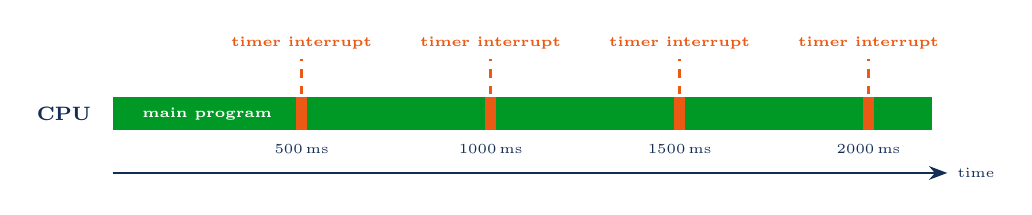
\begin{tikzpicture}[>=Stealth, font=\scriptsize]
    \node[anchor=east, font=\scriptsize\bfseries, text=DeepBlue] at (-0.15,0) {CPU};
    \fill[cWork] (0,-0.21) rectangle (10.4,0.21);
    \node[font=\tiny\bfseries, text=white] at (1.2,0) {main program};
    \foreach \k in {1,...,4} {
      \fill[cISR] ({2.4*\k-0.07},-0.21) rectangle ({2.4*\k+0.07},0.21);
      \draw[cISR, thick, dashed] ({2.4*\k},0.25) -- ({2.4*\k},0.7);
      \node[font=\tiny\bfseries, text=cISR] at ({2.4*\k},0.9) {timer interrupt};
      \node[font=\tiny, text=DeepBlue] at ({2.4*\k},-0.45) {\the\numexpr 500*\k\relax\,ms};
    }
    \draw[->, thick, DeepBlue] (0,-0.75) -- (10.6,-0.75) node[right, font=\tiny] {time};
  \end{tikzpicture}}

% ---------- one tick, three LEDs: #1 = number of ticks ----------
\newcommand{\tickleds}[1]{%
  \begin{tikzpicture}[font=\scriptsize]
    \pgfmathtruncatemacro{\tklast}{#1-1}
    \node[anchor=east, font=\scriptsize\bfseries, text=cISR] at (-0.15,0.55) {tick};
    \foreach \k in {1,...,#1} {
      \draw[cISR, very thick] ({0.42*\k},0.35) -- ({0.42*\k},0.75);
      \node[font=\tiny, text=DeepBlue] at ({0.42*\k},0.95) {\k};
    }
    \foreach \p/\r/\n in {3/1/LED 1, 5/2/LED 2, 7/3/LED 3} {
      \pgfmathsetmacro{\yy}{-0.6*\r+0.3}
      \node[anchor=east, font=\scriptsize\bfseries] at (-0.15,\yy+0.08) {\n};
      \node[anchor=east, font=\tiny, text=gray!40!black] at (-0.15,\yy-0.16) {every \p\ ticks};
      \foreach \k in {0,...,\tklast} {
        \pgfmathtruncatemacro{\s}{mod(floor(\k/\p),2)}
        \ifnum\s=1
          \fill[cLed!75] ({0.42*\k},\yy-0.17) rectangle ({0.42*(\k+1)},\yy+0.17);
        \else
          \fill[gray!12] ({0.42*\k},\yy-0.17) rectangle ({0.42*(\k+1)},\yy+0.17);
        \fi
      }
      \foreach \k in {1,...,#1} {
        \pgfmathtruncatemacro{\rr}{mod(\k,\p)}
        \ifnum\rr=0 \draw[cISR, very thick] ({0.42*\k},\yy-0.24) -- ({0.42*\k},\yy+0.24); \fi
      }
    }
    \draw[decorate, decoration={brace, amplitude=3pt, mirror}, thick, DeepBlue] (0.42,-1.8) -- (0.84,-1.8)
      node[midway, below=3pt, font=\tiny] {100 ms};
    \node[anchor=west, font=\tiny] at (2.0,-1.95) {\textcolor{cLed!75}{\rule{0.25cm}{0.2cm}}\ LED on
      \quad\textcolor{gray!25}{\rule{0.25cm}{0.2cm}}\ LED off
      \quad\textcolor{cISR}{\rule{0.06cm}{0.25cm}}\ the ISR changes the LED};
  \end{tikzpicture}}

% ---------- build it: two more LEDs (GPIO 7 and GPIO 3) ----------
% the circuit of Lecture 5 is faded, the new parts are drawn normally
\newcommand{\buildpicleds}{%
  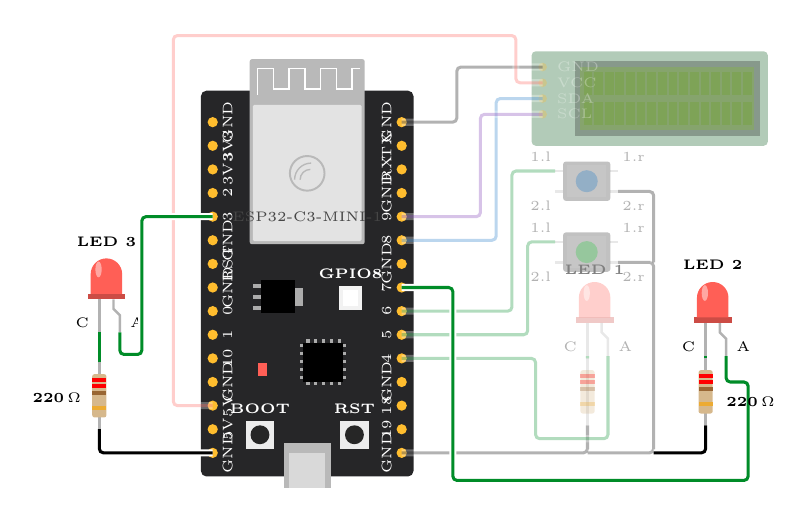
\begin{tikzpicture}[font=\tiny]
    \useasboundingbox (-2.2,-0.25) rectangle (7.3,5.7);
    \pic (esp) at (0,0) {esp32c3};
    \begin{scope}[opacity=0.3]
      % LED 1 and its resistor
      \pic (res) at (4.91,0.65) {wres};
      \pic (led) at (5.0,1.95) {wled};
      \draw[wire, black] (esp-R14) -- (4.91,0.3) -- (res-2);
      \draw[wire, WireGreen] (res-1) -- (led-C);
      \draw[wire, WireGreen] (esp-R10) -| (4.25,0.48) -| (led-A);
      % button A
      \pic (ba) at (4.9,2.85) {wbutton=MacGreen};
      \draw[wire, black] (ba-2r) -| (5.75,0.3) -- (4.91,0.3);
      \draw[wire, WireGreen] (esp-R9) -| ([xshift=-0.35cm]ba-1l) -- (ba-1l);
      % LCD
      \pic (lcd) at (4.2,4.2) {wlcd};
      \draw[wire, black] (esp-R0) -| ([xshift=-1.09cm]lcd-GND) -- (lcd-GND);
      \draw[wire, StorageBlue] (esp-R5) -| ([xshift=-0.59cm]lcd-SDA) -- (lcd-SDA);
      \draw[wire, ProgramPurple] (esp-R4) -| ([xshift=-0.79cm]lcd-SCL) -- (lcd-SCL);
      \draw[wire, MacRed] (esp-L12) -- (-0.35,0.9) -- (-0.35,5.6) -- (4.0,5.6) |- (lcd-VCC);
      % button B
      \pic (bb) at (4.9,3.75) {wbutton=StorageBlue};
      \draw[wire, black] (bb-2r) -| (5.75,2.72);
      \draw[wire, WireGreen] (esp-R8) -| ([xshift=-0.55cm]bb-1l) -- (bb-1l);
    \end{scope}
    \node[font=\fontsize{5.5}{6}\selectfont\bfseries, text=gray] at (5.0,2.62) {LED 1};
    % LED 2 on GPIO 7
    \pic (res2) at (6.41,0.65) {wres};
    \pic (led2) at (6.5,1.95) {wled};
    \draw[wire, black] (res2-2) -- (6.41,0.3) -- (5.75,0.3);
    \draw[wire, WireGreen] (res2-1) -- (led2-C);
    \draw[wire, WireGreen] (esp-R7) -- (3.2,2.4) -- (3.2,-0.05) -- (6.95,-0.05) -- (6.95,1.2) -- (6.67,1.2) -- (led2-A);
    \node[font=\fontsize{5.5}{6}\selectfont\bfseries, anchor=south] at (6.5,2.5) {LED 2};
    % LED 3 on GPIO 3
    \pic (res3) at (-1.29,0.6) {wres};
    \pic (led3) at (-1.2,2.25) {wled};
    \draw[wire, black] (res3-2) -- (-1.29,0.3) -- (esp-L14);
    \draw[wire, WireGreen] (res3-1) -- (led3-C);
    \draw[wire, WireGreen] (esp-L4) -- (-0.75,3.3) -- (-0.75,1.55) -- (-1.03,1.55) -- (led3-A);
    \node[font=\fontsize{5.5}{6}\selectfont\bfseries, anchor=south] at (-1.2,2.8) {LED 3};
    \node[font=\fontsize{5.5}{6}\selectfont\bfseries, anchor=east] at (-1.4,1.0) {220\,$\Omega$};
    \node[font=\fontsize{5.5}{6}\selectfont\bfseries, anchor=west] at (6.55,0.95) {220\,$\Omega$};
  \end{tikzpicture}}

% ---------- three LEDs, a button and the LCD (figure 2 of the course plan) ----------
\newcommand{\figthreeleds}{%
  \begin{tikzpicture}[>=Stealth, font=\scriptsize]
    \draw[DeepBlue, very thick, rounded corners=6pt, fill=DeepBlue!5] (0,-0.35) rectangle (4.0,3.75);
    \node[anchor=north west, font=\scriptsize\bfseries, text=DeepBlue] at (0.1,3.7) {\faMicrochip\ ESP32-C3};
    \node[lbox, draw=cISR, fill=cISR!15, minimum width=3.5cm, minimum height=0.8cm] (tisr) at (2.0,2.6)
      {Timer ISR\\[-1pt]{\mdseries every 100 ms: 3 LEDs}};
    \node[lbox, draw=cISR, fill=cISR!15, minimum width=3.5cm, minimum height=0.8cm] (bisr) at (2.0,1.5)
      {Button ISR\\[-1pt]{\ttfamily\mdseries presses++}};
    \node[lbox, draw=cWork, fill=cWork!12, minimum width=3.5cm, minimum height=0.8cm] (main) at (2.0,0.4)
      {main loop\\[-1pt]{\mdseries counts}};
    \foreach \y/\g/\n in {3.3/4/1, 2.6/7/2, 1.9/3/3} {
      \draw[->, thick, cISR] (tisr.east) -- (5.35,\y);
      \fill[cLed] (5.55,\y) circle (0.15);
      \node[anchor=west, font=\scriptsize] at (5.8,\y) {LED \n\ (GPIO \g)};
    }
    \node[lbox, draw=DeepBlue, fill=LightGray, minimum width=1.9cm] (btn) at (-1.9,1.5)
      {\faDotCircle\ Button A\\[-1pt]{\mdseries GPIO 5}};
    \draw[->, very thick, cISR] (btn.east) -- (bisr.west);
    \node[draw=mygreen!60!black, fill=mygreen!55!black, rounded corners=2pt, minimum width=2.6cm,
      minimum height=1.05cm] (lcd) at (6.4,0.4) {};
    \node[fill=LcdScreen!45, minimum width=2.3cm, minimum height=0.8cm, font=\ttfamily\scriptsize, align=left] at (lcd)
      {Presses: 3\\Loop: 18452};
    \draw[->, very thick, DeepBlue] (main.east) -- (lcd.west);
  \end{tikzpicture}}

% ---------- three ways to keep a rhythm: #1 = 1 delay(), 2 millis() in loop(), 3 timer interrupt ----------
\newcommand{\rhythm}[1]{%
  \begin{tikzpicture}[>=Stealth, font=\tiny]
    \useasboundingbox (-0.1,-1.0) rectangle (4.6,0.95);
    \ifnum#1=1
      \node[draw=white, fill=cIdle, minimum width=0.9cm, minimum height=0.42cm, inner sep=0pt, anchor=west,
        font=\tiny\bfseries, text=white] at (0,0) {LED 1};
      \node[draw=white, fill=cIdle, minimum width=1.5cm, minimum height=0.42cm, inner sep=0pt, anchor=west,
        font=\tiny\bfseries, text=white] at (0.9,0) {wait for LED 2};
      \node[draw=white, fill=cIdle, minimum width=2.1cm, minimum height=0.42cm, inner sep=0pt, anchor=west,
        font=\tiny\bfseries, text=white] at (2.4,0) {wait for LED 3};
      \node[font=\tiny\bfseries, text=DeepBlue, anchor=south] at (2.25,0.3) {\texttt{delay}: 300 + 500 + 700 ms, one after another};
      \draw[<->, thick, MacRed] (0,-0.45) -- node[below, font=\tiny\bfseries] {LED 1 changes again only after 1.5 s} (4.5,-0.45);
    \else
      \fill[cWork] (0,-0.21) rectangle (4.5,0.21);
      \foreach \a in {0.5,1.6,2.6,3.5} {
        \fill[cIdle] (\a,-0.21) rectangle (\a+0.6,0.21);
        \node[font=\tiny\bfseries, text=white] at (\a+0.3,0) {LCD};
      }
      \foreach \x in {0.9,1.8,2.7,3.6} \draw[DeepBlue, dashed, thick] (\x,0.25) -- (\x,0.6);
      \node[font=\tiny, text=DeepBlue, anchor=south] at (2.25,0.6) {when LED 1 should change};
    \fi
    \ifnum#1=2
      \foreach \x/\y in {0.9/1.1, 1.8/2.2, 2.7/3.2, 3.6/4.1} {
        \draw[MacRed, very thick] (\y,-0.28) -- (\y,-0.55);
        \draw[->, MacRed, thick] (\x,-0.42) -- (\y-0.03,-0.42);
      }
      \node[font=\tiny\bfseries, text=MacRed, anchor=north] at (2.25,-0.6) {LED 1 changes late: after each LCD write};
    \fi
    \ifnum#1=3
      \foreach \x in {0.9,1.8,2.7,3.6} {
        \fill[cISR] (\x-0.04,-0.21) rectangle (\x+0.04,0.21);
        \draw[cISR, very thick] (\x,-0.28) -- (\x,-0.55);
      }
      \node[font=\tiny\bfseries, text=cISR, anchor=north] at (2.25,-0.6) {LED 1 changes on time, even during the LCD write};
    \fi
  \end{tikzpicture}}

% ---------- one core, three tasks ----------
\newcommand{\oneprocessor}{%
  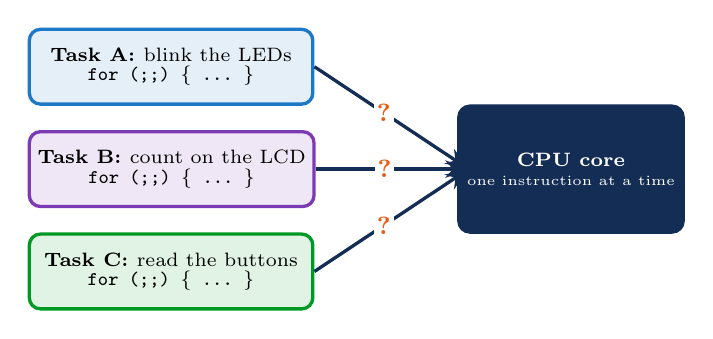
\begin{tikzpicture}[>=Stealth, font=\scriptsize]
    \foreach \n/\c/\w/\y in {A/cTaskA/blink the LEDs/1.3, B/cTaskB/count on the LCD/0, C/cTaskC/read the buttons/-1.3} {
      \node[lbox, draw=\c, fill=\c!12, minimum width=3.6cm, minimum height=0.95cm, anchor=west] (t\n) at (0,\y)
        {Task \n: {\mdseries \w}\\[-1pt]{\ttfamily\mdseries for (;;) \{ \ldots\ \}}};
      \draw[->, very thick, DeepBlue] (t\n.east) -- (5.6,0) node[pos=0.45, fill=white, font=\small\bfseries,
        text=AccentOrange, inner sep=1pt] {?};
    }
    \node[cpubox, minimum width=2.6cm, minimum height=1.6cm] at (6.9,0)
      {CPU core\\[-1pt]{\tiny\mdseries one instruction at a time}};
  \end{tikzpicture}}

% ---------- time slices, and how it looks to us ----------
\newcommand{\timeslices}{%
  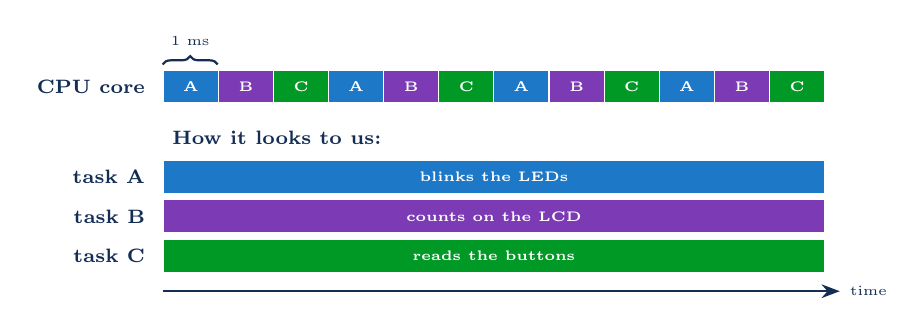
\begin{tikzpicture}[>=Stealth, font=\scriptsize]
    \tlbar{0}{CPU core}{0.7/cTaskA/A,0.7/cTaskB/B,0.7/cTaskC/C,0.7/cTaskA/A,0.7/cTaskB/B,0.7/cTaskC/C,
      0.7/cTaskA/A,0.7/cTaskB/B,0.7/cTaskC/C,0.7/cTaskA/A,0.7/cTaskB/B,0.7/cTaskC/C}
    \draw[decorate, decoration={brace, amplitude=3pt}, thick, DeepBlue] (0,0.28) -- (0.7,0.28)
      node[midway, above=3pt, font=\tiny] {1 ms};
    \node[anchor=west, font=\scriptsize\bfseries, text=DeepBlue] at (0,-0.65) {How it looks to us:};
    \tlbar{-1.15}{task A}{8.4/cTaskA/blinks the LEDs}
    \tlbar{-1.65}{task B}{8.4/cTaskB/counts on the LCD}
    \tlbar{-2.15}{task C}{8.4/cTaskC/reads the buttons}
    \draw[->, thick, DeepBlue] (0,-2.6) -- (8.6,-2.6) node[right, font=\tiny] {time};
  \end{tikzpicture}}

% ---------- the tick wakes the scheduler ----------
\newcommand{\tickscheduler}{%
  \begin{tikzpicture}[>=Stealth, font=\scriptsize]
    \node[lbox, draw=cISR, fill=cISR!15, minimum width=1.8cm, minimum height=0.9cm] (tim) at (0,0) {\faClock\ timer};
    \node[lbox, draw=cSched, fill=cSched!20, minimum width=2.3cm, minimum height=0.9cm] (sch) at (3.7,0)
      {scheduler\\[-1pt]{\tiny\mdseries which task next?}};
    \draw[->, very thick, cISR] (tim) -- node[above, font=\tiny\bfseries] {tick} node[below, font=\tiny] {every 1 ms} (sch);
    \node[lbox, draw=cTaskA, fill=cTaskA!12, minimum width=1.5cm] (a) at (7.0,1.0) {Task A};
    \node[lbox, draw=cTaskB, fill=cTaskB!25, minimum width=1.5cm, line width=2pt] (b) at (7.0,0) {Task B};
    \node[lbox, draw=cTaskC, fill=cTaskC!12, minimum width=1.5cm] (c) at (7.0,-1.0) {Task C};
    \draw[->, thick, DeepBlue!50] (sch.east) -- (a.west);
    \draw[->, line width=2pt, DeepBlue] (sch.east) -- (b.west);
    \draw[->, thick, DeepBlue!50] (sch.east) -- (c.west);
    \node[anchor=west, font=\tiny\bfseries, text=cTaskB] at (7.85,0) {runs now};
  \end{tikzpicture}}

% ---------- each task has its own stack ----------
\newcommand{\stackmem}{%
  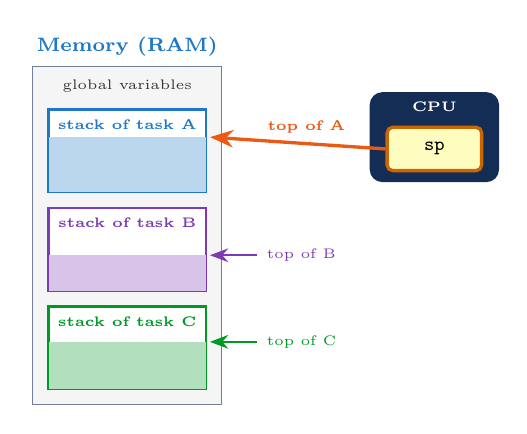
\begin{tikzpicture}[>=Stealth, font=\scriptsize]
    \node[font=\scriptsize\bfseries, text=StorageBlue] at (1.2,4.55) {Memory (RAM)};
    \draw[DeepBlue!60, fill=gray!8] (0,0) rectangle (2.4,4.3);
    \node[font=\tiny, text=gray!40!black] at (1.2,4.05) {global variables};
    \foreach \n/\c/\yb/\h in {A/cTaskA/2.7/0.7, B/cTaskB/1.45/0.45, C/cTaskC/0.2/0.6} {
      \draw[\c, thick, fill=white] (0.2,\yb) rectangle (2.2,\yb+1.05);
      \fill[\c!30] (0.2,\yb) rectangle (2.2,\yb+\h);
      \node[font=\tiny\bfseries, text=\c] at (1.2,\yb+0.86) {stack of task \n};
    }
    \foreach \n/\c/\t in {B/cTaskB/1.9, C/cTaskC/0.8} {
      \draw[->, thick, \c] (2.85,\t) -- (2.25,\t);
      \node[anchor=west, font=\tiny, text=\c] at (2.85,\t) {top of \n};
    }
    \node[cpubox, minimum width=1.6cm, minimum height=1.1cm] (cpu) at (5.1,3.4) {};
    \node[font=\tiny\bfseries, text=white, anchor=north] at (cpu.north) {CPU};
    \node[reg, minimum width=1.2cm] (sp) at (5.1,3.25) {\textbf{sp}};
    \draw[->, very thick, AccentOrange] (sp.west) -- (2.25,3.4) node[pos=0.45, above, font=\tiny\bfseries] {top of A};
  \end{tikzpicture}}

% ---------- context switch in 4 steps ----------
% #1 = step (1 tick, 2 save A, 3 choose B, 4 restore B)
\newcommand{\ctxswitch}[1]{%
  \begin{tikzpicture}[>=Stealth, font=\scriptsize,
      cell/.style={draw=DeepBlue!50, minimum width=1.8cm, minimum height=0.42cm, inner sep=0pt, font=\ttfamily\tiny},
      src/.style={draw=ReadBlue, line width=1.6pt},
      dst/.style={draw=WriteRed, line width=1.6pt},
      tcell/.style={draw=DeepBlue!50, fill=white, minimum height=0.45cm, inner sep=0pt}]
    \useasboundingbox (-0.2,-0.7) rectangle (12.5,4.75);
    % ----- the CPU -----
    \draw[DeepBlue, very thick, rounded corners=6pt, fill=DeepBlue!6] (0,0) rectangle (3.0,3.6);
    \node[anchor=north west, font=\scriptsize\bfseries, text=DeepBlue] at (0.08,3.55) {CPU};
    \ifcase#1 \or \def\running{task A}\or \def\running{scheduler}\or \def\running{scheduler}\or \def\running{task B}\fi
    \node[anchor=north east, font=\tiny] at (2.95,3.55) {running: \textbf{\running}};
    \ifnum#1<4 \colorlet{ctxc}{cTaskA}\def\who{A}\else \colorlet{ctxc}{cTaskB}\def\who{B}\fi
    \foreach \r/\y in {PC/2.75, t0/2.1, t1/1.45} {
      \node[draw=ctxc, very thick, fill=ctxc!12, rounded corners=2pt, minimum width=2.4cm, minimum height=0.48cm,
        font=\ttfamily\scriptsize] at (1.5,\y) {\textbf{\r}\ \ \who's \r};
    }
    \node[draw=ctxc, very thick, fill=ctxc!12, rounded corners=2pt, minimum width=2.4cm, minimum height=0.48cm,
      font=\ttfamily\scriptsize] at (1.5,0.55) {\textbf{sp}\ \ top of \who};
    \ifnum#1=2
      \draw[src, rounded corners=3pt] (0.22,1.14) rectangle (2.78,3.06);
      \draw[src, rounded corners=3pt] (0.22,0.24) rectangle (2.78,0.86);
    \fi
    \ifnum#1=4
      \draw[dst, rounded corners=3pt] (0.22,1.14) rectangle (2.78,3.06);
      \draw[dst, rounded corners=3pt] (0.22,0.24) rectangle (2.78,0.86);
    \fi
    % ----- the two stacks -----
    \foreach \sx/\n/\c in {4.9/A/cTaskA, 7.6/B/cTaskB} {
      \node[font=\scriptsize\bfseries, text=\c] at (\sx,3.3) {stack of \n};
      \draw[\c, thick] (\sx-0.95,0.15) rectangle (\sx+0.95,3.0);
      \node[cell, fill=\c!8, font=\tiny] at (\sx,0.45) {data of \n};
      \node[cell, fill=\c!8, font=\tiny] at (\sx,0.87) {data of \n};
    }
    \ifnum#1>1
      \foreach \r/\y in {t1/1.29, t0/1.71, PC/2.13} \node[cell, fill=cTaskA!30] at (4.9,\y) {A's \r};
    \else
      \foreach \y in {1.29,1.71,2.13} \node[cell, draw=DeepBlue!25, dashed] at (4.9,\y) {};
    \fi
    \ifnum#1=2 \draw[dst, rounded corners=2pt] (3.98,1.06) rectangle (5.82,2.36); \fi
    \foreach \r/\y in {t1/1.29, t0/1.71, PC/2.13} \node[cell, fill=cTaskB!30] at (7.6,\y) {B's \r};
    \ifnum#1=4 \draw[src, rounded corners=2pt] (6.68,1.06) rectangle (8.52,2.36); \fi
    % top of each stack
    \ifnum#1>1 \def\topA{2.34}\else \def\topA{1.08}\fi
    \ifnum#1>3 \def\topB{1.08}\else \def\topB{2.34}\fi
    \draw[->, thick, cTaskA] (6.15,\topA) -- (5.88,\topA);
    \node[anchor=west, font=\tiny, text=cTaskA] at (6.12,\topA) {top};
    \draw[->, thick, cTaskB] (8.85,\topB) -- (8.58,\topB);
    \node[anchor=west, font=\tiny, text=cTaskB] at (8.82,\topB) {top};
    % ----- the table of saved stack pointers -----
    \node[draw=DeepBlue, fill=DeepBlue, text=white, font=\tiny\bfseries, minimum width=2.6cm, minimum height=0.42cm]
      at (10.7,3.0) {saved sp};
    \ifnum#1>1 \def\valA{top of A}\else \def\valA{--}\fi
    \node[tcell, minimum width=0.9cm, font=\tiny\bfseries, text=cTaskA] at (9.85,2.55) {task A};
    \node[tcell, minimum width=1.7cm, font=\ttfamily\tiny] (va) at (11.15,2.55) {\valA};
    \node[tcell, minimum width=0.9cm, font=\tiny\bfseries, text=cTaskB] at (9.85,2.1) {task B};
    \node[tcell, minimum width=1.7cm, font=\ttfamily\tiny] (vb) at (11.15,2.1) {top of B};
    \ifnum#1=2 \draw[dst] (va.south west) rectangle (va.north east); \fi
    \ifnum#1=3 \draw[cSched, line width=1.6pt] (9.4,1.875) rectangle (12.0,2.325); \fi
    \ifnum#1=4 \draw[src] (vb.south west) rectangle (vb.north east); \fi
    % ----- legend -----
    \node[font=\tiny, anchor=west] at (4.1,4.4) {\textcolor{ReadBlue}{\rule{0.25cm}{0.2cm}}\ read from here
      \quad\textcolor{WriteRed}{\rule{0.25cm}{0.2cm}}\ written here
      \quad\textcolor{cTaskA}{\rule{0.25cm}{0.2cm}}\ task A
      \quad\textcolor{cTaskB}{\rule{0.25cm}{0.2cm}}\ task B};
    % ----- what happens in this step -----
    \ifnum#1=1
      \node[lbox, draw=cISR, fill=cISR!15] (tick) at (1.5,4.3) {\faClock\ tick: timer interrupt};
      \draw[->, very thick, cISR] (tick) -- (1.5,3.62);
    \fi
    \ifnum#1=2
      \draw[->, very thick, DeepBlue] (2.8,2.1) -- (3.96,1.71);
      \draw[->, very thick, DeepBlue, rounded corners=3pt] (2.8,0.55) -- (3.4,0.55) -- (3.4,-0.45) -- (12.3,-0.45)
        -- (12.3,2.55) -- (12.02,2.55);
    \fi
    \ifnum#1=3
      \node[lbox, draw=cSched, fill=cSched!20] (sch) at (10.7,1.1) {scheduler: next task = B};
      \draw[->, very thick, cSched] (sch) -- (10.7,1.86);
    \fi
    \ifnum#1=4
      \draw[->, very thick, DeepBlue, rounded corners=3pt] (12.02,2.1) -- (12.3,2.1) -- (12.3,-0.45) -- (3.4,-0.45)
        -- (3.4,0.55) -- (2.82,0.55);
      \draw[->, very thick, DeepBlue, rounded corners=3pt] (8.54,1.71) -- (9.0,1.71) -- (9.0,3.75) -- (3.3,3.75)
        -- (3.3,2.1) -- (2.82,2.1);
    \fi
  \end{tikzpicture}}
\newcommand{\ctxlegend}{%
  {\tiny\textcolor{ReadBlue}{\rule{0.25cm}{0.2cm}}\ read from here
  \qquad\textcolor{WriteRed}{\rule{0.25cm}{0.2cm}}\ written here
  \qquad\textcolor{cTaskA}{\rule{0.25cm}{0.2cm}}\ task A
  \qquad\textcolor{cTaskB}{\rule{0.25cm}{0.2cm}}\ task B}}

% ---------- task states ----------
\newcommand{\taskstates}{%
  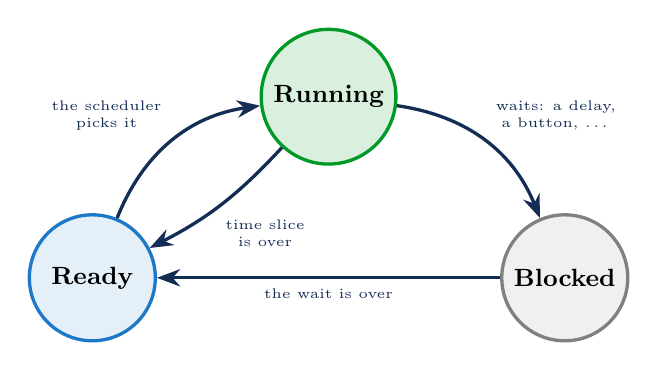
\begin{tikzpicture}[>=Stealth, font=\scriptsize,
      st/.style={circle, very thick, minimum size=1.6cm, font=\small\bfseries, align=center}]
    \node[st, draw=mygreen, fill=mygreen!15] (run) at (0,2.3) {Running};
    \node[st, draw=StorageBlue, fill=StorageBlue!12] (rdy) at (-3.0,0) {Ready};
    \node[st, draw=gray, fill=gray!12] (blk) at (3.0,0) {Blocked};
    \draw[->, very thick, DeepBlue] (rdy) to[bend left=30] node[above left, font=\tiny, align=center] {the scheduler\\picks it} (run);
    \draw[->, very thick, DeepBlue] (run) to[bend left=10] node[below right, font=\tiny, align=center, pos=0.55] {time slice\\is over} (rdy);
    \draw[->, very thick, DeepBlue] (run) to[bend left=30] node[above right, font=\tiny, align=center] {waits: a delay,\\a button, \ldots} (blk);
    \draw[->, very thick, DeepBlue] (blk) -- node[below, font=\tiny] {the wait is over} (rdy);
  \end{tikzpicture}}

% ---------- round robin and priorities ----------
\newcommand{\rrqueue}{%
  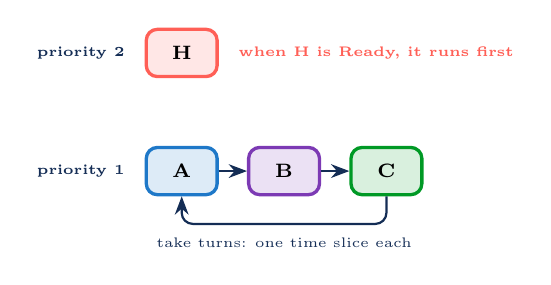
\begin{tikzpicture}[>=Stealth, font=\scriptsize, tk/.style={lbox, minimum width=0.9cm, minimum height=0.6cm}]
    \node[font=\tiny\bfseries, text=DeepBlue, anchor=east] at (-0.6,1.5) {priority 2};
    \node[tk, draw=cTaskH, fill=cTaskH!15] (h) at (0,1.5) {H};
    \node[anchor=west, font=\tiny\bfseries, text=cTaskH] at (0.6,1.5) {when H is Ready, it runs first};
    \node[font=\tiny\bfseries, text=DeepBlue, anchor=east] at (-0.6,0) {priority 1};
    \node[tk, draw=cTaskA, fill=cTaskA!15] (a) at (0,0) {A};
    \node[tk, draw=cTaskB, fill=cTaskB!15] (b) at (1.3,0) {B};
    \node[tk, draw=cTaskC, fill=cTaskC!15] (c) at (2.6,0) {C};
    \draw[->, thick, DeepBlue] (a) -- (b);
    \draw[->, thick, DeepBlue] (b) -- (c);
    \draw[->, thick, DeepBlue, rounded corners=4pt] (c.south) -- ++(0,-0.35) -| (a.south);
    \node[font=\tiny, text=DeepBlue, anchor=north] at (1.3,-0.72) {take turns: one time slice each};
  \end{tikzpicture}}

% ---------- FreeRTOS on our ESP32-C3 ----------
\newcommand{\rtostasks}{%
  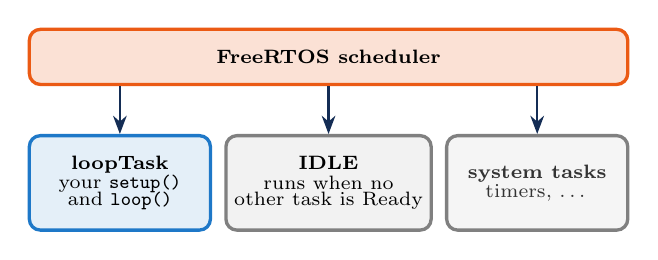
\begin{tikzpicture}[>=Stealth, font=\scriptsize]
    \node[lbox, draw=cSched, fill=cSched!18, minimum width=7.6cm, minimum height=0.7cm] (s) at (0,1.6) {FreeRTOS scheduler};
    \node[lbox, draw=cTaskA, fill=cTaskA!12, minimum width=2.3cm, minimum height=1.2cm] (l) at (-2.65,0)
      {loopTask\\[-1pt]{\mdseries your \texttt{setup()}}\\[-2pt]{\mdseries and \texttt{loop()}}};
    \node[lbox, draw=gray, fill=gray!10, minimum width=2.3cm, minimum height=1.2cm] (i) at (0,0)
      {IDLE\\[-1pt]{\mdseries runs when no}\\[-2pt]{\mdseries other task is Ready}};
    \node[greybox, minimum width=2.3cm, minimum height=1.2cm] (y) at (2.65,0)
      {system tasks\\[-1pt]{\mdseries timers, \ldots}};
    \foreach \t in {l,i,y} \draw[->, thick, DeepBlue] (s.south -| \t) -- (\t.north);
  \end{tikzpicture}}

% ---------- the Ready lists of FreeRTOS ----------
\newcommand{\readylists}{%
  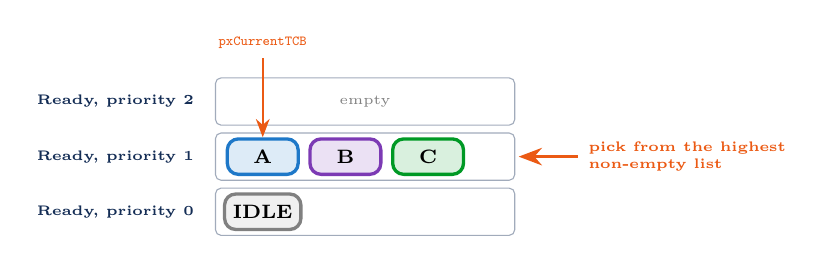
\begin{tikzpicture}[>=Stealth, font=\scriptsize, tk/.style={lbox, minimum width=0.9cm, minimum height=0.45cm}]
    \foreach \p/\y in {2/1.0, 1/0.3, 0/-0.4} {
      \node[font=\tiny\bfseries, text=DeepBlue, anchor=east] at (-0.15,\y) {Ready, priority \p};
      \draw[DeepBlue!40, rounded corners=2pt] (0,\y-0.3) rectangle (3.8,\y+0.3);
    }
    \node[font=\tiny, text=gray] at (1.9,1.0) {empty};
    \node[tk, draw=cTaskA, fill=cTaskA!15] (a) at (0.6,0.3) {A};
    \node[tk, draw=cTaskB, fill=cTaskB!15] at (1.65,0.3) {B};
    \node[tk, draw=cTaskC, fill=cTaskC!15] at (2.7,0.3) {C};
    \node[tk, draw=gray, fill=gray!12] at (0.6,-0.4) {IDLE};
    \draw[<-, very thick, cSched] (3.85,0.3) -- (4.6,0.3) node[right, font=\tiny\bfseries, align=left]
      {pick from the highest\\non-empty list};
    \node[font=\tiny\ttfamily, text=cSched, anchor=south] (cur) at (0.6,1.55) {pxCurrentTCB};
    \draw[->, thick, cSched] (cur.south) to[out=-90, in=90] (a.north);
  \end{tikzpicture}}

% ---------- two tasks, one counter ----------
\newcommand{\racetimeline}{%
  \begin{tikzpicture}[>=Stealth, font=\scriptsize]
    \node[anchor=east, font=\scriptsize\bfseries, text=cTaskA] at (-0.15,0.5) {Task A};
    \node[anchor=east, font=\scriptsize\bfseries, text=cTaskB] at (-0.15,0) {Task B};
    \foreach \k in {0,...,6} {
      \fill[cTaskA] ({1.2*\k},0.29) rectangle ({1.2*\k+0.6},0.71);
      \fill[cTaskB] ({1.2*\k+0.6},-0.21) rectangle ({1.2*\k+1.2},0.21);
    }
    \node[font=\tiny\bfseries, text=white] at (0.3,0.5) {\texttt{++}};
    \node[font=\tiny\bfseries, text=white] at (0.9,0) {\texttt{++}};
    \draw[MacRed, very thick, dashed] (3.0,-0.4) -- (3.0,1.1);
    \node[font=\large, text=MacRed] at (3.0,1.35) {\faBolt};
    \node[font=\tiny\bfseries, text=MacRed, anchor=west] at (3.25,1.35) {a switch at a bad moment: some updates are lost};
    \draw[->, thick, DeepBlue] (0,-0.55) -- (8.6,-0.55) node[right, font=\tiny] {time};
    \node[font=\tiny, anchor=north] at (4.2,-0.65) {one time slice = 1 ms: thousands of \texttt{counter++} each};
  \end{tikzpicture}}

% ---------- only one task at a time may update the counter ----------
\newcommand{\lockbox}{%
  \begin{tikzpicture}[>=Stealth, font=\scriptsize]
    \node[draw=AccentOrange, very thick, rounded corners=4pt, fill=AccentOrange!10, minimum width=3.8cm,
      minimum height=1.4cm, align=center] (cs) at (0,0)
      {{\Large\textcolor{AccentOrange}{\faLock}}\\[3pt]\texttt{counter++;}};
    \node[font=\tiny\bfseries, text=AccentOrange, anchor=north] at ([yshift=-2pt]cs.south) {must not be interrupted by the other task};
    \node[lbox, draw=cTaskA, fill=cTaskA!12, minimum width=1.6cm] (a) at (-4.2,0.45) {Task A};
    \node[lbox, draw=cTaskB, fill=cTaskB!12, minimum width=1.6cm] (b) at (-4.2,-0.45) {Task B};
    \draw[->, very thick, cTaskA] (a.east) -- (cs.west |- a.east) node[pos=0.5, above, font=\tiny] {inside};
    \draw[->, very thick, cTaskB] (b.east) -- (-2.45,-0.45);
    \node[font=\tiny, text=cTaskB, anchor=north] at (-2.75,-0.6) {\faHourglassHalf\ waits};
  \end{tikzpicture}}

\title{Computer Hardware}
\subtitle{A Brief History of Concurrency: From a Button to a Scheduler}
\author{Ksawery Możdżyński}
\date{}

\begin{document}

\begin{frame}
  \titlepage
\end{frame}

\begin{frame}{Agenda For Today}
  \Large
  \begin{itemize}
    \item[\textcolor{AccentOrange}{\faBolt}] \textbf{1. Interrupts} \\
    \textcolor{gray}{\small The device tells the processor that something happened}
    \vspace{0.3cm}

    \item[\textcolor{AccentOrange}{\faRandom}] \textbf{2. The scheduler} \\
    \textcolor{gray}{\small One processor, several tasks}
    \vspace{0.3cm}

    \item[\textcolor{AccentOrange}{\faMicrochip}] \textbf{3. FreeRTOS} \\
    \textcolor{gray}{\small A real scheduler on the ESP32-C3}
  \end{itemize}
\end{frame}

\begin{frame}{Today you will need}
  \begin{columns}[c,onlytextwidth]
    \column{0.48\textwidth}
      \begin{beamercolorbox}[rounded=true,sep=0.16cm,wd=\linewidth]{block body}
        \centering\large\textbf{Wokwi}\\[0.1cm]
        {\Huge\textcolor{DeepBlue}{\faMicrochip}}\\[0.15cm]
        \normalsize\texttt{wokwi.com}\\[0.05cm]
        \footnotesize your project \projCircuit\ from Lecture 5
      \end{beamercolorbox}
    \column{0.48\textwidth}
      \begin{beamercolorbox}[rounded=true,sep=0.16cm,wd=\linewidth]{block body}
        \centering\large\textbf{ConcurrencySimulator}\\[0.1cm]
        {\Huge\textcolor{DeepBlue}{\faMousePointer}}\\[0.15cm]
        \normalsize\simurl\\[0.05cm]
        \footnotesize new: made for today
      \end{beamercolorbox}
  \end{columns}
  \vfill
  \keymsg{Please open both now. All day we do the same thing: \textbf{a short talk, then you try it}.}
\end{frame}

\begin{frame}{From last time: polling}
  \begin{columns}[c,onlytextwidth]
    \column{0.55\textwidth}
      \centering
      {\scriptsize\textbf{Task 7}: 2 s of work, then one check\par}
      \vspace{0.1cm}
      \begin{tikzpicture}
        \tlbar{0}{CPU}{1.4/cWork/work,0.25/cPoll/?,1.4/cWork/work,0.25/cPoll/?,1.4/cWork/work,0.25/cPoll/?}
        \foreach \x/\ok in {0.6/0, 1.52/1, 2.4/0, 3.9/0} {
          \ifnum\ok=1 \def\cc{HitGreen}\else\def\cc{MissRed}\fi
          \node[font=\scriptsize, text=\cc] at (\x,0.55) {\faDotCircle};
          \draw[\cc, thick, dashed] (\x,0.4) -- (\x,0.22);
        }
        \node[font=\tiny, text=DeepBlue, anchor=west] at (5.05,0.55) {presses};
      \end{tikzpicture}\\[0.3cm]
      {\scriptsize\textbf{Task 8}: nothing but checks\par}
      \vspace{0.1cm}
      \begin{tikzpicture}
        \tlbar{0}{CPU}{0.31/cPoll/?,0.31/cPoll/?,0.31/cPoll/?,0.31/cPoll/?,0.31/cPoll/?,0.31/cPoll/?,0.31/cPoll/?,0.31/cPoll/?,
          0.31/cPoll/?,0.31/cPoll/?,0.31/cPoll/?,0.31/cPoll/?,0.31/cPoll/?,0.31/cPoll/?,0.31/cPoll/?,0.31/cPoll/?}
        \node[font=\tiny, text=white] at (5.05,0) {.};
      \end{tikzpicture}\\[0.2cm]
      \cpulegend
    \column{0.42\textwidth}
      \stepbox{Check rarely (Task 7)}{Short presses were \textbf{lost}: the LCD showed fewer than 5, often 0 or 1.}
      \stepbox{Check all the time (Task 8)}{Nothing was lost, but more than \textbf{99.99\%} of the checks found nothing.}
  \end{columns}
  \vfill
  \keymsg{Better idea: let the \textbf{button tell the processor} when it is pressed.}
\end{frame}

% =====================================================================
\section{Interrupts}
% =====================================================================

\begin{frame}{An interrupt}
  \defbox{An \textbf{interrupt} is a signal from a device to the processor:
    \emph{something happened, deal with it now}.}
  \vspace{0.15cm}
  \begin{center}
    \irqtimeline
  \end{center}
  \vfill
  \keymsg{\textbf{ISR} = Interrupt Service Routine: a short function that the processor runs when the interrupt arrives.}
\end{frame}

\begin{frame}{What happens inside the processor}
  \begin{columns}[c,onlytextwidth]
    \column{0.56\textwidth}
      \centering
      \resizebox{\linewidth}{!}{%
        \only<1>{\irqsteps{1}}%
        \only<2>{\irqsteps{2}}%
        \only<3>{\irqsteps{3}}%
        \only<4>{\irqsteps{4}}%
      }\\[0.15cm]
      {\scriptsize\textcolor{gray}{In RISC-V the saved PC is kept in a special register, \texttt{mepc}.}\par}
    \column{0.42\textwidth}
      \stepbox{\badge{1}\ Signal}{Button A raises an interrupt signal while the CPU runs \texttt{addi}.}
      \uncover<2->{\stepbox{\badge{2}\ Save and jump}{The CPU \textbf{finishes} \texttt{addi}, \textbf{saves the PC}
        (the address of the next instruction) and jumps to the ISR.}}
      \uncover<3->{\stepbox{\badge{3}\ The ISR runs}{It saves \texttt{t0}, does its work and restores \texttt{t0}.}}
      \uncover<4->{\stepbox{\badge{4}\ Return}{The CPU \textbf{restores the PC}: the main program continues with \texttt{sw}.}}
  \end{columns}
  \vfill
  \uncover<4->{\keymsg{The main program \textbf{does not know} that it was interrupted.}}
\end{frame}

% SIMULATOR (topic "Polling vs interrupt"): the same as in DeviceSimulator, without bouncing.
% SIMULATOR (topic "Interrupt step by step"): the main program below; the signal from button A
%   arrives during the instruction at 0x0108; the ISR saves t0 on the stack and restores it.
\begin{frame}[fragile]{Simulator 1: polling and interrupts}
  \begin{columns}[T,onlytextwidth]
    \column{0.49\textwidth}
      \taskhead{Simulator task}{Open \simname, topic \simtab{Polling vs interrupt}.}
      \footnotesize
      \begin{enumerate}\setlength{\itemsep}{4pt}
        \item Mode \emph{2 s of work, then one check}. Click \textbf{Start}, then \textbf{5 short clicks}.
          How many presses does polling count? And the interrupt?
        \item Look at the row \emph{CPU: interrupts}. How much of the CPU time went to the ISR?
      \end{enumerate}
    \column{0.48\textwidth}
      \taskhead{Then}{Topic \simtab{Interrupt step by step}. The signal from button A arrives
        \textbf{during} the instruction at \texttt{0x0108}.}
\begin{lstlisting}[style=rv6]
0x0100  li   t0, 0
0x0104  addi t0, t0, 1
0x0108  sw   t0, 0(a0)
0x010C  j    0x0104
\end{lstlisting}
      \footnotesize
      \begin{enumerate}\setcounter{enumi}{2}\setlength{\itemsep}{4pt}
        \item \textbf{Predict} the saved PC. Then step through and check.
        \item The ISR uses \texttt{t0}. What is \texttt{t0} in the main program after the return?
      \end{enumerate}
  \end{columns}
\end{frame}

\begin{frame}{Solution: Simulator 1}
  \begin{columns}[T,onlytextwidth]
    \column{0.48\textwidth}
      \stepbox{Question 1}{Polling: usually \textbf{0 or 1}. A click counts only if it happens exactly during a check.
        Interrupt: \textbf{5}.}
      \stepbox{Question 2}{Almost \textbf{nothing}. Each ISR takes a few microseconds:
        on the timeline it is only a thin orange line.}
    \column{0.48\textwidth}
      \stepbox{Question 3}{\texttt{0x010C}. The CPU first finishes \texttt{sw}, so the saved PC is the address of the
        \textbf{next} instruction.}
      \stepbox{Question 4}{The same as before the interrupt. The ISR saved \texttt{t0} on the stack and restored it
        before the return.}
  \end{columns}
  \vfill
  \keymsg{An interrupt misses nothing, costs almost no CPU time, and the main program continues
    \textbf{exactly where it stopped}.}
\end{frame}

\begin{frame}{The button with an interrupt}
  \begin{center}
    \resizebox{0.85\textwidth}{!}{\figbuttonisr}
  \end{center}
  \vfill
  \keymsg{The main program only \textbf{shows} the number. It never checks the button.}
\end{frame}

\begin{frame}[fragile]{Interrupts in the code}
  \begin{columns}[c,onlytextwidth]
    \column{0.53\textwidth}
\begin{lstlisting}[style=rtos]
const int BUTTON_A = 5;
volatile int presses = 0;

void IRAM_ATTR onButtonA() {     // the ISR
  presses++;
}

void setup() {
  pinMode(BUTTON_A, INPUT_PULLUP);
  attachInterrupt(digitalPinToInterrupt(BUTTON_A),
                  onButtonA, FALLING);
}
\end{lstlisting}
    \column{0.44\textwidth}
      \stepbox{\texttt{attachInterrupt}}{Call \texttt{onButtonA} on a \texttt{FALLING} edge: when the pin goes
        from 1 to 0, i.e.\ when the button is \textbf{pressed}.}
      \stepbox{\texttt{IRAM\_ATTR}}{Keep the ISR in fast internal memory. Required on the ESP32.}
      \stepbox{\texttt{volatile}}{As in Lecture 5: really read the variable every time.
        The ISR can change it ``behind the program's back''.}
  \end{columns}
\end{frame}

\begin{frame}[fragile]{Task 1: count the presses}
  \begin{columns}[T,onlytextwidth]
    \column{0.5\textwidth}
\begin{lstlisting}[style=rtos]
#include <Wire.h>
#include <LiquidCrystal_I2C.h>
LiquidCrystal_I2C lcd(0x27, 16, 2);

const int BUTTON_A = 5;
volatile int presses = 0;
// TODO: the ISR

void setup() {
  Wire.begin(8, 9);
  lcd.init();  lcd.backlight();
  // TODO: the pin and the interrupt
}

void loop() {
  // TODO: show "Presses: N"
}
\end{lstlisting}
    \column{0.47\textwidth}
      \taskhead{Task}{Open your project \projCircuit\ from Lecture 5: button A on GPIO 5, LCD on GPIO 8/9.}
      \footnotesize
      \begin{enumerate}\setlength{\itemsep}{4pt}
        \item Count the presses of button A \textbf{with an interrupt}.
        \item Show the number on the LCD: \texttt{Presses: N}.
        \item Add \texttt{delay(2000)} to \texttt{loop()}, as in Task 7 of Lecture 5.
          Do you still lose any presses? Why not?
      \end{enumerate}
      \vspace{0.1cm}
      \begin{beamercolorbox}[rounded=true,sep=0.1cm,wd=\linewidth]{block body}
        \scriptsize\textbf{If you finish early:} give button B (GPIO 6) its own interrupt that sets the counter
        back to 0.
      \end{beamercolorbox}
  \end{columns}
\end{frame}

\begin{frame}[fragile]{Solution: count the presses}
  \begin{columns}[T,onlytextwidth]
    \column{0.55\textwidth}
\begin{lstlisting}[style=rtos]
void IRAM_ATTR onButtonA() { presses++; }

void setup() {
  Wire.begin(8, 9);
  lcd.init();  lcd.backlight();
  pinMode(BUTTON_A, INPUT_PULLUP);
  attachInterrupt(digitalPinToInterrupt(BUTTON_A),
                  onButtonA, FALLING);
}

void loop() {
  lcd.setCursor(0, 0);
  lcd.print("Presses: ");
  lcd.print(presses);
  lcd.print("   ");          // clear old digits
  delay(2000);
}
\end{lstlisting}
    \column{0.42\textwidth}
      \stepbox{Question 3}{\textbf{No} press is lost. The interrupt counts it even while \texttt{loop()} waits.
        The LCD just shows the new number up to 2 s later.}
      \stepbox{Compare with Task 7}{The same \texttt{delay(2000)}, but now nothing is missed.}
      \stepbox{If you finished early}{\texttt{onButtonB()} sets \texttt{presses = 0}. Attach it to pin 6
        with \texttt{FALLING}, like button A.}
  \end{columns}
\end{frame}

\begin{frame}{Rules for an ISR}
  \begin{columns}[T,onlytextwidth]
    \column{0.31\textwidth}
      \stepbox{\badge{1}\ Keep it short}{While the ISR runs, the main program waits.}
    \column{0.31\textwidth}
      \stepbox{\badge{2}\ No slow work inside}{No \texttt{delay()}, no printing to the LCD or to Serial.}
    \column{0.31\textwidth}
      \stepbox{\badge{3}\ Share data through \texttt{volatile} variables}{The ISR changes them, the main program reads them.}
  \end{columns}
  \vspace{0.3cm}
  \begin{center}
    \begin{tikzpicture}[>=Stealth]
      \node[lbox, draw=cISR, fill=cISR!15, minimum width=3.4cm, minimum height=0.9cm] (isr) at (0,0)
        {ISR\\[-1pt]{\mdseries records what happened}};
      \node[lbox, draw=cWork, fill=cWork!12, minimum width=3.4cm, minimum height=0.9cm] (main) at (6,0)
        {main program\\[-1pt]{\mdseries does the slow work}};
      \draw[->, very thick, DeepBlue] (isr) -- node[above, font=\scriptsize\ttfamily] {volatile presses} (main);
    \end{tikzpicture}
  \end{center}
  \vfill
  \keymsg{The ISR only \textbf{records} what happened. The main program \textbf{does the work}.}
\end{frame}

\begin{frame}{Interrupts from a timer}
  \defbox{A \textbf{timer} is a counter inside the processor. When it reaches a set value, it raises an interrupt:
    again and again, at regular intervals.}
  \vspace{0.3cm}
  \begin{center}
    \timertimeline
  \end{center}
  \vfill
  \keymsg{A timer interrupt lets the processor do something \textbf{regularly}, without checking the time in the main program.}
\end{frame}

% CHECK before class: the timer API below is the one of the ESP32 core 3.x used by Wokwi.
% Core 2.x would need: timerBegin(0, 80, true), timerAttachInterrupt(timer, &onTimer, true),
% timerAlarmWrite(timer, 500000, true), timerAlarmEnable(timer).
\begin{frame}[fragile]{A timer in the code}
  \begin{columns}[c,onlytextwidth]
    \column{0.56\textwidth}
\begin{lstlisting}[style=rtos]
const int LED = 4;
hw_timer_t *timer = nullptr;
volatile bool ledOn = false;

void IRAM_ATTR onTimer() {        // the ISR
  ledOn = !ledOn;
  digitalWrite(LED, ledOn);
}

void setup() {
  pinMode(LED, OUTPUT);
  timer = timerBegin(1000000);          // 1 step = 1 us
  timerAttachInterrupt(timer, &onTimer);
  timerAlarm(timer, 500000, true, 0);   // every 500 ms
}
\end{lstlisting}
    \column{0.41\textwidth}
      \stepbox{\texttt{timerBegin(1000000)}}{The timer counts at 1 MHz: one step every 1\,$\mu$s.}
      \stepbox{\texttt{timerAttachInterrupt}}{When the alarm goes off, call \texttt{onTimer}.}
      \stepbox{\texttt{timerAlarm}}{Alarm after 500\,000 steps = 500 ms, and \textbf{repeat} it (\texttt{true}).}
  \end{columns}
  \vfill
  \keymsg{The LED blinks with \textbf{no code in} \texttt{loop()}: the timer calls \texttt{onTimer} every 500 ms.}
\end{frame}

\begin{frame}{Three LEDs, three rhythms, one timer}
  \begin{beamercolorbox}[rounded=true,sep=0.1cm,wd=\textwidth]{block body}
    \centering\small Three LEDs should change every \textbf{300}, \textbf{500} and \textbf{700 ms}.
    But the ESP32-C3 has only \textbf{two} hardware timers.
  \end{beamercolorbox}
  \vspace{0.15cm}
  \begin{center}
    \tickleds{21}
  \end{center}
  \vspace{-0.1cm}
  \defbox{One timer interrupt at a fixed rate is called a \textbf{tick}. Here: a tick every 100 ms.
    At every tick, the ISR \textbf{decides} what to do: LED 1 every 3 ticks, LED 2 every 5, LED 3 every 7.}
\end{frame}

\begin{frame}[fragile]{The tick in the code}
  \begin{columns}[c,onlytextwidth]
    \column{0.62\textwidth}
\begin{lstlisting}[style=rtos]
volatile unsigned long ticks = 0;
volatile bool led1 = false, led2 = false, led3 = false;

void IRAM_ATTR onTick() {        // every 100 ms
  ticks++;
  if (ticks % 3 == 0) { led1 = !led1; digitalWrite(LED1, led1); }
  if (ticks % 5 == 0) { led2 = !led2; digitalWrite(LED2, led2); }
  if (ticks % 7 == 0) { led3 = !led3; digitalWrite(LED3, led3); }
}
\end{lstlisting}
    \column{0.35\textwidth}
      \stepbox{\texttt{ticks \% 3 == 0}}{Every third tick: 300 ms.}
      \stepbox{One timer}{\texttt{timerAlarm(timer, 100000, true, 0)}: a tick every 100 ms.}
  \end{columns}
  \vfill
  \keymsg{Remember this idea: a \textbf{regular tick}, and a \textbf{decision} at every tick. We will need it in Part 2.}
\end{frame}

% SIMULATOR (topic "Timer and tick"): a tick every 100 ms, LEDs change every 3, 5 and 7 ticks,
%   all LEDs are off at the start; the user can step tick by tick.
\begin{frame}{Simulator 2: the tick}
  \taskhead{Simulator task}{Topic \simtab{Timer and tick}: a tick every 100 ms. LED 1 changes every 3 ticks,
    LED 2 every 5, LED 3 every 7. At the start all LEDs are off. \textbf{Predict first}, then check.}
  \begin{columns}[T,onlytextwidth]
    \column{0.5\textwidth}
      \footnotesize
      \begin{enumerate}\setlength{\itemsep}{5pt}
        \item Which LEDs change at tick \textbf{15}? At tick \textbf{21}? At tick \textbf{35}?
        \item Which LEDs are \textbf{on} right after tick \textbf{10}?
        \item At which tick do all three change \textbf{together} for the first time? After how many seconds?
      \end{enumerate}
    \column{0.46\textwidth}
      \centering\footnotesize
      \renewcommand{\arraystretch}{1.25}
      \begin{tabular}{cccc}
        \toprule
        & \textbf{LED 1} & \textbf{LED 2} & \textbf{LED 3} \\
        \midrule
        changes at tick 15 & \ldots & \ldots & \ldots \\
        changes at tick 21 & \ldots & \ldots & \ldots \\
        changes at tick 35 & \ldots & \ldots & \ldots \\
        on after tick 10 & \ldots & \ldots & \ldots \\
        \bottomrule
      \end{tabular}
  \end{columns}
\end{frame}

\begin{frame}{Solution: Simulator 2}
  \begin{columns}[c,onlytextwidth]
    \column{0.52\textwidth}
      \centering\footnotesize
      \renewcommand{\arraystretch}{1.25}
      \begin{tabular}{cccc}
        \toprule
        & \textbf{LED 1} & \textbf{LED 2} & \textbf{LED 3} \\
        \midrule
        changes at tick 15 & \textcolor{HitGreen}{\faCheck} & \textcolor{HitGreen}{\faCheck} & -- \\
        changes at tick 21 & \textcolor{HitGreen}{\faCheck} & -- & \textcolor{HitGreen}{\faCheck} \\
        changes at tick 35 & -- & \textcolor{HitGreen}{\faCheck} & \textcolor{HitGreen}{\faCheck} \\
        on after tick 10 & \textbf{on} & off & \textbf{on} \\
        \bottomrule
      \end{tabular}
    \column{0.45\textwidth}
      \stepbox{Question 2}{LED 1 changed 3 times (ticks 3, 6, 9): on. LED 2 twice (5, 10): off. LED 3 once (7): on.}
      \stepbox{Question 3}{At tick $3 \times 5 \times 7 = \mathbf{105}$, after \textbf{10.5 s}.}
  \end{columns}
  \vfill
  \keymsg{A LED changes when the tick number is divisible by its period: the ISR checks this at every tick.}
\end{frame}

\begin{frame}{Build it: two more LEDs}
  \begin{columns}[c,onlytextwidth]
    \column{0.56\textwidth}
      \centering
      \resizebox{\linewidth}{!}{\buildpicleds}
    \column{0.42\textwidth}
      \stepbox{\badge{1}\ Parts}{Click \textbf{+}, add two \textbf{LEDs} and two \textbf{Resistors} (220\,$\Omega$).}
      \stepbox{\badge{2}\ Wires}{GPIO \textbf{7} $\to$ LED 2 \textsf{A}.\ \ GPIO \textbf{3} $\to$ LED 3 \textsf{A}.
        Each \textsf{C} $\to$ resistor $\to$ \textbf{GND}.}
      \stepbox{\badge{3}\ Keep it}{The LED on GPIO 4 is now \textbf{LED 1}. Save the project.}
  \end{columns}
  \vfill
  \keymsg{Our circuit now: LEDs on GPIO 4, 7 and 3; buttons on 5 and 6; LCD on 8 and 9.}
\end{frame}

\begin{frame}{Task 2: three LEDs}
  \begin{columns}[c,onlytextwidth]
    \column{0.5\textwidth}
      \centering
      \resizebox{\linewidth}{!}{\figthreeleds}
    \column{0.47\textwidth}
      \taskhead{Task}{Use the circuit with three LEDs (or the project \projLeds\ from the course page).}
      \footnotesize
      \begin{enumerate}\setlength{\itemsep}{4pt}
        \item Make LED 1 blink every 500 ms \textbf{with a timer interrupt}, as on the slide ``A timer in the code''.
        \item Change it: one tick every \textbf{100 ms}, and the three LEDs change every 300, 500 and 700 ms.
        \item Keep the button counter from Task 1. In \texttt{loop()}, also count as fast as possible and show
          \texttt{Loop: N} in row 1. Do the LEDs keep their rhythm?
      \end{enumerate}
      \vspace{0.05cm}
      \begin{beamercolorbox}[rounded=true,sep=0.1cm,wd=\linewidth]{block body}
        \scriptsize\textbf{If you finish early:} make LED 1 blink with \texttt{millis()} in \texttt{loop()}
        instead of the timer, and keep the LCD writes. Is its rhythm still even?
      \end{beamercolorbox}
  \end{columns}
\end{frame}

\begin{frame}[fragile]{Solution: three LEDs}
  \begin{columns}[T,onlytextwidth]
    \column{0.56\textwidth}
\begin{lstlisting}[style=rtos]
const int LED1 = 4, LED2 = 7, LED3 = 3;
long loops = 0;
void setup() {
  // the LCD and button A as in Task 1
  pinMode(LED1, OUTPUT);  pinMode(LED2, OUTPUT);
  pinMode(LED3, OUTPUT);
  timer = timerBegin(1000000);
  timerAttachInterrupt(timer, &onTick);
  timerAlarm(timer, 100000, true, 0);  // 100 ms
}

void loop() {
  loops++;
  lcd.setCursor(0, 0);
  lcd.print("Presses: ");  lcd.print(presses);
  lcd.setCursor(0, 1);
  lcd.print("Loop: ");     lcd.print(loops);
}
\end{lstlisting}
    \column{0.41\textwidth}
      \stepbox{The ISR}{\texttt{onTick} from the slide ``The tick in the code''.}
      \stepbox{Question 3}{\textbf{Yes}. The LEDs and the button are handled by interrupts, so it does not matter what
        \texttt{loop()} does, even slow LCD writes.}
  \end{columns}
\end{frame}

% SIMULATOR (topic "Timer and tick", second mode): switch "How" with delay(), millis() in loop(),
%   timer interrupt; a switch "loop() writes to the LCD" (one write = several ms).
\begin{frame}[fragile]{Simulator 3: could we do this without interrupts?}
  \begin{columns}[T,onlytextwidth]
    \column{0.49\textwidth}
      {\scriptsize\textbf{With \texttt{delay()}}\par}
\begin{lstlisting}[style=rtos]
void loop() {
  digitalWrite(LED1, HIGH);  delay(300);
  digitalWrite(LED1, LOW);   delay(300);
  // and LED 2? LED 3?
}
\end{lstlisting}
      {\scriptsize\textbf{With \texttt{millis()}}\par}
\begin{lstlisting}[style=rtos]
void loop() {
  if (millis() - last1 >= 300) {
    last1 += 300;  toggle(LED1);
  }
  // the same for LED 2 and LED 3
  showOnLcd();              // several ms
}
\end{lstlisting}
    \column{0.48\textwidth}
      \taskhead{Simulator task}{Topic \simtab{Timer and tick}, switch \emph{How}: \texttt{delay()},
        \texttt{millis()} in \texttt{loop()} or a timer interrupt. Turn on \emph{loop() writes to the LCD}.}
      \footnotesize
      \begin{enumerate}\setlength{\itemsep}{5pt}
        \item \texttt{delay()}: do the LEDs keep 300, 500 and 700 ms?
        \item \texttt{millis()} in \texttt{loop()}: look at the moments when LED 1 changes. Are they on time?
        \item Timer interrupt: are they on time now?
      \end{enumerate}
  \end{columns}
\end{frame}

\begin{frame}{Solution: Simulator 3}
  \begin{columns}[T,onlytextwidth]
    \column{0.31\textwidth}
      \centering
      \resizebox{\linewidth}{!}{\rhythm{1}}\\[0.1cm]
      \stepbox{1. \texttt{delay()}}{\textbf{No}. While the CPU waits for one LED, it cannot serve the others.
        The waits add up.}
    \column{0.31\textwidth}
      \centering
      \resizebox{\linewidth}{!}{\rhythm{2}}\\[0.1cm]
      \stepbox{2. \texttt{millis()}}{Almost. But each slow step in the loop delays the LEDs: the rhythm is
        \textbf{uneven}.}
    \column{0.31\textwidth}
      \centering
      \resizebox{\linewidth}{!}{\rhythm{3}}\\[0.1cm]
      \stepbox{3. Timer interrupt}{\textbf{Yes}. The tick comes on time, whatever the loop is doing.}
  \end{columns}
  \vfill
  {\centering\scriptsize\textcolor{gray}{\texttt{millis()} in \texttt{loop()} is polling again:
    the loop keeps asking ``is it time yet?''.}\par}
  \vspace{0.05cm}
  \keymsg{Without interrupts it is possible, but it is \textbf{hard to keep an exact rhythm}
    while the program also does other work.}
\end{frame}

\begin{frame}{Interrupts: summary}
  \begin{center}
    \small
    \renewcommand{\arraystretch}{1.4}
    \begin{tabular}{ll}
      \toprule
      \textbf{Polling} & \textbf{Interrupts} \\
      \midrule
      the processor \textbf{asks} the device & the device \textbf{tells} the processor \\
      short events can be missed & nothing is missed \\
      wastes time on checking & the processor works until something happens \\
      a rhythm is hard to keep & a timer gives an exact rhythm \\
      \bottomrule
    \end{tabular}
  \end{center}
  \vfill
  \keymsg{Our tick decided \textbf{which LED} to change. Next: what if the tick decided \textbf{which program} runs?}
\end{frame}

% =====================================================================
\section{The scheduler}
% =====================================================================

\begin{frame}{One processor, several tasks}
  \begin{beamercolorbox}[rounded=true,sep=0.12cm,wd=\textwidth]{block body}
    \small In Task 2 each LED needed only a tiny piece of work, so it fit into the ISR.
    But real tasks are \textbf{long programs} with their own loops and waits: read a sensor, update the LCD,
    talk over Wi-Fi. They cannot run inside a short ISR.
  \end{beamercolorbox}
  \vspace{0.2cm}
  \begin{center}
    \oneprocessor
  \end{center}
  \vfill
  \keymsg{How can three programs, each with its own endless loop, share \textbf{one core}?}
\end{frame}

\begin{frame}{The idea: take turns very quickly}
  \begin{center}
    \timeslices
  \end{center}
  \vspace{0.05cm}
  \begin{columns}[T,onlytextwidth]
    \column{0.48\textwidth}
      \stepbox{Time slice}{Each task runs for a short \textbf{time slice}, then the next one gets the core.
        The switches are so fast that all tasks seem to run at the same time.}
    \column{0.48\textwidth}
      \defbox{\textbf{Concurrency}: several tasks make progress by \textbf{taking turns} on one core.}
      {\scriptsize\textcolor{gray}{Several cores working at the same moment: \emph{parallelism}. More on Tuesday.}\par}
  \end{columns}
\end{frame}

\begin{frame}{Who decides when to switch?}
  \defbox{The \textbf{scheduler} is the part of the system that decides \textbf{which task runs next} and switches to it.}
  \vspace{0.15cm}
  \begin{columns}[c,onlytextwidth]
    \column{0.66\textwidth}
      \centering
      \resizebox{\linewidth}{!}{\tickscheduler}
    \column{0.31\textwidth}
      \stepbox{Task 2}{tick $\to$ \textbf{which LED}?}
      \stepbox{The scheduler}{tick $\to$ \textbf{which task}?}
  \end{columns}
  \vfill
  \keymsg{The same idea as in Task 2: a regular \textbf{tick}, and a decision at every tick.
    On our ESP32 the tick comes every \textbf{1 ms}.}
\end{frame}

% SIMULATOR (topic "Time slice"): tasks A, B, C, round robin, time slice adjustable (1 ms ... 500 ms);
%   two rows: what the core really does, and how it looks to us (A blinks an LED, B counts, C reads buttons).
\begin{frame}{Simulator 4: time slices}
  \taskhead{Simulator task}{Topic \simtab{Time slice}: tasks A, B and C take turns (round robin), one time slice = 1 ms.
    Task A starts at 0 ms. \textbf{Predict first}, then check.}
  \footnotesize
  \begin{enumerate}\setlength{\itemsep}{6pt}
    \item Which task runs from \textbf{7 to 8 ms}?
    \item How many task switches happen in \textbf{one second}?
    \item Set the time slice to \textbf{500 ms}. Look at the row \emph{how it looks to us}.
      Do the tasks still seem to run at the same time?
  \end{enumerate}
\end{frame}

\begin{frame}{Solution: Simulator 4}
  \begin{center}
    \begin{tikzpicture}[>=Stealth, font=\scriptsize]
      \tlbar{0}{CPU core}{0.8/cTaskA/A,0.8/cTaskB/B,0.8/cTaskC/C,0.8/cTaskA/A,0.8/cTaskB/B,0.8/cTaskC/C,
        0.8/cTaskA/A,0.8/cTaskB/B,0.8/cTaskC/C}
      \foreach \k in {0,...,9} \node[font=\tiny, text=DeepBlue] at ({0.8*\k},-0.4) {\k};
      \node[font=\tiny, text=DeepBlue, anchor=west] at (7.35,-0.4) {ms};
      \draw[AccentOrange, very thick, rounded corners=2pt] (5.6,-0.27) rectangle (6.4,0.27);
    \end{tikzpicture}
  \end{center}
  \vspace{0.1cm}
  \begin{columns}[T,onlytextwidth]
    \column{0.31\textwidth}
      \stepbox{Question 1}{\textbf{B}: A, B, C, A, B, C, A, \textbf{B}.}
    \column{0.31\textwidth}
      \stepbox{Question 2}{\textbf{1000}: one switch every 1 ms.}
    \column{0.31\textwidth}
      \stepbox{Question 3}{\textbf{No}. Now you can see them take turns: the LED stops for a whole second
        while B and C run.}
  \end{columns}
  \vfill
  \keymsg{Concurrency works because the time slices are \textbf{short}: much shorter than anything we can notice.}
\end{frame}

\begin{frame}{What does a task need to continue later?}
  \begin{beamercolorbox}[rounded=true,sep=0.12cm,wd=\textwidth]{block body}
    \centering\small If we stop task A now and resume it later, \textbf{what must we remember}?
  \end{beamercolorbox}
  \vspace{0.25cm}
  \begin{columns}[T,onlytextwidth]
    \column{0.31\textwidth}
      \uncover<2->{\qcard{\faMapMarker}{\textbf{PC}\\ where the task stopped: the next instruction}}
    \column{0.31\textwidth}
      \uncover<3->{\qcard{\faMicrochip}{\textbf{Registers}\\ the values it was working with, e.g.\ \texttt{x5}, \texttt{x6} in Ripes}}
    \column{0.31\textwidth}
      \uncover<4->{\qcard{\faLayerGroup}{\textbf{Stack}\\ its local variables and the functions it is in}}
  \end{columns}
  \vspace{0.25cm}
  \uncover<4->{\defbox{Together this is the task's \textbf{context}.}}
  \vfill
  \uncover<4->{\keymsg{The ISR in Simulator 1 already saved \texttt{t0}: the same idea, but now we save \textbf{everything}.}}
\end{frame}

\begin{frame}{Each task has its own stack}
  \begin{columns}[c,onlytextwidth]
    \column{0.5\textwidth}
      \centering
      \stackmem
    \column{0.47\textwidth}
      \stepbox{Its own stack}{Each task has \textbf{its own stack} in memory: its local variables and saved registers.}
      \stepbox{The register \texttt{sp}}{The stack pointer points to the stack of the task that is \textbf{running now}.}
  \end{columns}
  \vfill
  \keymsg{To switch tasks: save the registers on the old task's stack and \textbf{change} \texttt{sp}.}
\end{frame}

\begin{frame}{Context switch, step by step}
  \begin{center}
    \resizebox{!}{0.64\textheight}{%
      \only<1>{\ctxswitch{1}}%
      \only<2>{\ctxswitch{2}}%
      \only<3>{\ctxswitch{3}}%
      \only<4>{\ctxswitch{4}}%
    }
  \end{center}
  \vspace{-0.15cm}
  \only<1>{\stepbox{\badge{1}\ Tick}{Task A runs. The timer interrupt arrives and the CPU jumps to the scheduler.}}
  \only<2>{\stepbox{\badge{2}\ Save A}{A's registers and PC go onto \textbf{stack A}. The new top of stack A goes
    into the table of saved stack pointers.}}
  \only<3>{\stepbox{\badge{3}\ Choose B}{The scheduler picks the next task: \textbf{B}.}}
  \only<4>{\stepbox{\badge{4}\ Restore B}{\texttt{sp} $\leftarrow$ the saved sp of B. B's registers and PC come back
    from stack B: B continues as if nothing happened. These 4 steps are a \textbf{context switch}.}}
\end{frame}

% SIMULATOR (topic "Context switch"): the 4 steps of the slide before, with these values:
%   CPU: PC = 0x0210, t0 = 7, t1 = 3, sp = 0x2000 (task A runs);
%   stack B holds B's saved context: PC = 0x0308, t0 = 42, t1 = 9; saved sp of B = 0x2FF4;
%   a context is 3 registers (PC, t0, t1) of 4 bytes, so saving moves sp down by 12 = 0xC.
\begin{frame}{Simulator 5: a context switch}
  \taskhead{Simulator task}{Topic \simtab{Context switch}. \textbf{Before each step}, predict what will change.
    Then click \textbf{Next} and check.}
  \begin{columns}[T,onlytextwidth]
    \column{0.45\textwidth}
      \centering\footnotesize\textbf{At the start}\\[0.1cm]
      \scriptsize
      \renewcommand{\arraystretch}{1.2}
      \begin{tabular}{lll}
        \toprule
        & \textcolor{cTaskA}{\textbf{CPU (task A runs)}} & \textcolor{cTaskB}{\textbf{saved on stack B}} \\
        \midrule
        \texttt{PC} & \texttt{0x0210} & \texttt{0x0308} \\
        \texttt{t0} & \texttt{7}      & \texttt{42} \\
        \texttt{t1} & \texttt{3}      & \texttt{9} \\
        \texttt{sp} & \texttt{0x2000} & saved sp of B: \texttt{0x2FF4} \\
        \bottomrule
      \end{tabular}\\[0.15cm]
      \raggedright Each register takes \textbf{4 bytes}. A context = \texttt{PC}, \texttt{t0}, \texttt{t1}.
    \column{0.52\textwidth}
      \footnotesize
      \begin{enumerate}\setlength{\itemsep}{5pt}
        \item Step 2, \emph{Save A}: which values go onto stack A? What is the saved sp of A?
        \item Step 4, \emph{Restore B}: what are \texttt{PC}, \texttt{t0}, \texttt{t1} and \texttt{sp} after the restore?
        \item Where is A's \texttt{t0 = 7} now? Who gives it back to A, and when?
      \end{enumerate}
  \end{columns}
\end{frame}

\begin{frame}{Solution: Simulator 5}
  \begin{columns}[T,onlytextwidth]
    \column{0.31\textwidth}
      \stepbox{Question 1}{\texttt{0x0210}, \texttt{7} and \texttt{3}: 3 registers $\times$ 4 bytes = 12 = \texttt{0xC}.\\[0.05cm]
        Saved sp of A: \texttt{0x2000} $-$ \texttt{0xC} = \textbf{\texttt{0x1FF4}}.}
    \column{0.31\textwidth}
      \stepbox{Question 2}{\texttt{PC} = \texttt{0x0308}, \texttt{t0} = \texttt{42}, \texttt{t1} = \texttt{9}.\\[0.05cm]
        \texttt{sp} = \texttt{0x2FF4} + \texttt{0xC} = \textbf{\texttt{0x3000}}.}
    \column{0.31\textwidth}
      \stepbox{Question 3}{On \textbf{stack A}. The scheduler restores it at the next switch back to A,
        exactly like B's values now.}
  \end{columns}
  \vfill
  \keymsg{Task A will never notice the break: its \texttt{t0} waits for it on its own stack.}
\end{frame}

\begin{frame}{Task states}
  \begin{columns}[c,onlytextwidth]
    \column{0.56\textwidth}
      \centering
      \resizebox{\linewidth}{!}{\taskstates}
    \column{0.41\textwidth}
      \stepbox{Running}{On one core only \textbf{one} task runs at a time.}
      \stepbox{Ready}{Could run, waits for its turn.}
      \stepbox{Blocked}{Waits for something: a delay, a button. Gets \textbf{no} time slices.}
      \stepbox{Nobody is Ready?}{Then the CPU runs a special task that does nothing: \textbf{IDLE}.}
  \end{columns}
  \vfill
  \keymsg{A Blocked task uses \textbf{no processor time}, unlike polling.}
\end{frame}

\begin{frame}{Which task runs next?}
  \begin{columns}[c,onlytextwidth]
    \column{0.47\textwidth}
      \stepbox{Round robin}{Tasks with the \textbf{same priority} take turns, one time slice each.}
      \stepbox{Priorities}{A Ready task with a \textbf{higher priority} always runs first.
        It even stops (preempts) a running task with a lower priority.}
    \column{0.5\textwidth}
      \centering
      \resizebox{0.95\linewidth}{!}{\rrqueue}
  \end{columns}
  \vfill
  \keymsg{The scheduler picks the Ready task with the \textbf{highest priority}; equal priorities take turns.}
\end{frame}

% SIMULATOR (topic "States and priorities"): A, B, C priority 1 (round robin, 1 ms), H priority 2 waits
%   for the button; C calls a 3 ms delay at 2 ms; a CPU usage bar that includes the IDLE task.
% SIMULATOR (topic "Shared counter"): two tasks, each does counter++ three times, the counter starts at 0;
%   the moments of the switches are random, so some runs give 4 or 5. Do NOT show the read and the write
%   of counter++ separately: the explanation is on Tuesday.
\begin{frame}{Simulator 6: states, priorities and a shared counter}
  \begin{columns}[T,onlytextwidth]
    \column{0.52\textwidth}
      \taskhead{Simulator task}{Topic \simtab{States and priorities}: A, B and C have priority 1.
        Task H has priority 2 and waits for the button.}
      \footnotesize
      \begin{enumerate}\setlength{\itemsep}{4pt}
        \item At 2 ms, task C calls a 3 ms delay. In which state is C from 2 to 5 ms? Does it get any time slices?
        \item Press the button: H becomes Ready. What happens to the task that is running?
        \item What runs when A, B and C are all Blocked?
      \end{enumerate}
    \column{0.45\textwidth}
      \taskhead{Then}{Topic \simtab{Shared counter}: two tasks, each adds 1 to \texttt{counter} three times.
        The counter starts at 0.}
      \footnotesize
      \begin{enumerate}\setcounter{enumi}{3}\setlength{\itemsep}{4pt}
        \item \textbf{Predict} the final value.
        \item Click \textbf{Run} three times and write down the results.
      \end{enumerate}
  \end{columns}
\end{frame}

\begin{frame}{Solution: Simulator 6}
  \begin{columns}[T,onlytextwidth]
    \column{0.48\textwidth}
      \stepbox{Question 1}{\textbf{Blocked}: no time slices. At 5 ms it becomes Ready again.}
      \stepbox{Question 2}{It is stopped at once and goes to Ready. \textbf{H} runs.
        When H waits again, A, B and C continue.}
      \stepbox{Question 3}{The \textbf{IDLE} task.}
    \column{0.48\textwidth}
      \stepbox{Questions 4 and 5}{We expect \textbf{6}. But some runs give \textbf{4} or \textbf{5},
        and the result changes from run to run.}
      \probbox{Some additions were lost}{Two tasks, six additions, and the counter did not count them all. Why?
        Keep this question: we will meet it again at the end of today.}
  \end{columns}
\end{frame}

% =====================================================================
\section{FreeRTOS}
% =====================================================================

\begin{frame}{A real scheduler: FreeRTOS}
  \defbox{\textbf{FreeRTOS} is a small operating system for microcontrollers: mainly a \textbf{scheduler}
    plus tools that help tasks cooperate.}
  \vspace{0.2cm}
  \begin{columns}[T,onlytextwidth]
    \column{0.31\textwidth}
      \stepbox{\faCode\ Free and open}{Open source. Runs on many processors, including RISC-V.}
    \column{0.31\textwidth}
      \stepbox{\faStopwatch\ RTOS}{\emph{Real-time operating system}: a task with a high priority reacts quickly.}
    \column{0.31\textwidth}
      \stepbox{\faMicrochip\ Everywhere}{Sensors, home appliances, cars, \ldots}
  \end{columns}
  \vfill
  \keymsg{Everything from Part 2 is inside: the tick, time slices, states, priorities and the context switch.}
\end{frame}

\begin{frame}{You have used FreeRTOS all along}
  \begin{columns}[c,onlytextwidth]
    \column{0.55\textwidth}
      \centering
      \resizebox{\linewidth}{!}{\rtostasks}
    \column{0.42\textwidth}
      \stepbox{\texttt{loopTask}}{On the ESP32, your \texttt{setup()} and \texttt{loop()} already run
        \textbf{inside a FreeRTOS task}.}
      \stepbox{\texttt{delay()} = \texttt{vTaskDelay()}}{On the ESP32, \texttt{delay()} makes the task
        \textbf{Blocked}: while your \texttt{loop()} waited, it did not waste the CPU.}
  \end{columns}
  \vfill
  \keymsg{Nothing to install: we can create our own tasks.}
\end{frame}

\begin{frame}[fragile]{Task 3: who runs \texttt{loop()}?}
  \begin{columns}[T,onlytextwidth]
    \column{0.5\textwidth}
\begin{lstlisting}[style=rtos]
void setup() {
  Serial.begin(115200);
  Serial.print("Task: ");
  Serial.println(pcTaskGetName(NULL));
  Serial.print("Priority: ");
  Serial.println(uxTaskPriorityGet(NULL));
}

void loop() {
  delay(1000);
}
\end{lstlisting}
    \column{0.47\textwidth}
      \taskhead{Task}{Any Wokwi project: replace \texttt{setup()} and \texttt{loop()} with this code.
        Run it and open the \textbf{Serial Monitor}.}
      \footnotesize
      \begin{enumerate}\setlength{\itemsep}{4pt}
        \item Which task runs \texttt{setup()}?
        \item What is its priority?
      \end{enumerate}
      \vspace{0.1cm}
      \scriptsize\texttt{NULL} means: the task that is running now.
  \end{columns}
\end{frame}

\begin{frame}[fragile]{Solution: who runs \texttt{loop()}?}
  \begin{columns}[c,onlytextwidth]
    \column{0.45\textwidth}
      {\scriptsize\textbf{Serial Monitor}\par}
\begin{lstlisting}[style=term]
Task: @loopTask@
Priority: @1@
\end{lstlisting}
    \column{0.5\textwidth}
      \stepbox{Questions 1 and 2}{The task \textbf{loopTask}, with priority \textbf{1}.}
      \stepbox{Next}{The tasks we create will also get priority 1, so they take turns with \texttt{loopTask}.}
  \end{columns}
\end{frame}

\begin{frame}[fragile]{Creating a task: \texttt{xTaskCreate}}
  \begin{columns}[c,onlytextwidth]
    \column{0.52\textwidth}
\begin{lstlisting}[style=rtos]
void blinkTask(void *param) {
  for (;;) {                       // forever
    digitalWrite(LED1, HIGH);
    vTaskDelay(pdMS_TO_TICKS(500));
    digitalWrite(LED1, LOW);
    vTaskDelay(pdMS_TO_TICKS(500));
  }
}

void setup() {
  pinMode(LED1, OUTPUT);
  xTaskCreate(blinkTask, "blink", 2048, NULL, 1, NULL);
}
\end{lstlisting}
    \column{0.45\textwidth}
      \centering\scriptsize
      \textbf{The arguments of \texttt{xTaskCreate}}\\[0.1cm]
      \renewcommand{\arraystretch}{1.2}
      \begin{tabular}{@{}ll@{}}
        \toprule
        \texttt{blinkTask} & the task function: an endless loop \\
        \texttt{"blink"} & a name, for debugging \\
        \texttt{2048} & stack size, on the ESP32 in \textbf{bytes} \\
        \texttt{NULL} & a parameter for the task \\
        \texttt{1} & the priority \\
        \texttt{NULL} & a handle (not needed here) \\
        \bottomrule
      \end{tabular}
  \end{columns}
  \vfill
  \keymsg{\texttt{vTaskDelay} makes the task \textbf{Blocked}: it uses no processor time while it waits.}
\end{frame}

% CHECK in Wokwi before class: with a busy task the IDLE task gets no time; a "task watchdog" message
% may appear in the Serial Monitor after a few seconds. If it does, show it: the system notices it.
\begin{frame}[fragile]{Task 4: three LEDs as three tasks}
  \begin{columns}[T,onlytextwidth]
    \column{0.52\textwidth}
      \taskhead{Task}{The same three LEDs as in Task 2, but now \textbf{without the timer}.}
      \footnotesize
      \begin{enumerate}\setlength{\itemsep}{4pt}
        \item Remove the timer. Create \textbf{three tasks} with \texttt{xTaskCreate}: LED 1 changes every 300 ms,
          LED 2 every 500 ms, LED 3 every 700 ms.
        \item Keep \texttt{Loop: N} on the LCD in \texttt{loop()}. Do the LEDs keep their rhythm?
        \item In the task of LED 3, replace \texttt{vTaskDelay} with a \textbf{busy wait} (on the right).
          Do the other LEDs still blink? Now create this task with priority \textbf{2}. What happens?
      \end{enumerate}
    \column{0.45\textwidth}
      {\scriptsize\textbf{A busy wait for question 3}\par}
\begin{lstlisting}[style=rtos]
unsigned long t = millis();
while (millis() - t < 700) { }
\end{lstlisting}
      \vspace{0.1cm}
      \stepbox{Hint}{One function can serve all three tasks: pass the pin and the period through \texttt{param}.}
      \begin{beamercolorbox}[rounded=true,sep=0.1cm,wd=\linewidth]{block body}
        \scriptsize\textbf{If you finish early:} replace \texttt{vTaskDelay} with \texttt{vTaskDelayUntil}.
        What is the difference?
      \end{beamercolorbox}
  \end{columns}
\end{frame}

\begin{frame}[fragile]{Solution: three LEDs as three tasks}
  \begin{columns}[T,onlytextwidth]
    \column{0.5\textwidth}
\begin{lstlisting}[style=rtos]
struct Blink { int pin; int ms; };
Blink b1 = {4, 300}, b2 = {7, 500}, b3 = {3, 700};

void blinkTask(void *param) {
  Blink *b = (Blink *)param;
  pinMode(b->pin, OUTPUT);
  for (;;) {
    digitalWrite(b->pin, HIGH);
    vTaskDelay(pdMS_TO_TICKS(b->ms));
    digitalWrite(b->pin, LOW);
    vTaskDelay(pdMS_TO_TICKS(b->ms));
  }
}

// in setup():
xTaskCreate(blinkTask, "led1", 2048, &b1, 1, NULL);
xTaskCreate(blinkTask, "led2", 2048, &b2, 1, NULL);
xTaskCreate(blinkTask, "led3", 2048, &b3, 1, NULL);
\end{lstlisting}
    \column{0.47\textwidth}
      \stepbox{Question 2}{\textbf{Yes}. Each LED task is Blocked most of the time and gets the core
        within 1 ms when its delay is over.}
      \stepbox{Question 3, priority 1}{The other LEDs still blink, but the busy task wastes its time slices:
        \textbf{polling again}.}
      \stepbox{Question 3, priority 2}{The other LEDs and the LCD \textbf{stop}: the busy task is always Ready
        and has the highest priority.}
      \stepbox{If you finished early}{\texttt{vTaskDelayUntil} wakes the task at fixed moments: small delays do not add up.}
  \end{columns}
\end{frame}

\begin{frame}{Two solutions of the same problem}
  \begin{center}
    \small
    \renewcommand{\arraystretch}{1.4}
    \begin{tabular}{lll}
      \toprule
      & \textbf{Task 2: one timer + ticks} & \textbf{Task 4: three FreeRTOS tasks} \\
      \midrule
      Who counts the ticks & you, in the ISR & the scheduler \\
      The code of one LED & mixed into one ISR & its own simple loop \\
      A fourth LED & change the ISR & one more \texttt{xTaskCreate} \\
      Waiting & -- & \texttt{vTaskDelay}: Blocked, no CPU \\
      Cost & nothing extra & one stack per task (RAM) \\
      \bottomrule
    \end{tabular}
  \end{center}
  \vfill
  \keymsg{Both use a timer tick. With FreeRTOS, the scheduler does the bookkeeping for you.
    Next: \textbf{look inside}, what did it do?}
\end{frame}

% Source: FreeRTOS kernel, tasks.c (simplified). CHECK the version you show; ESP-IDF has its own copy.
\begin{frame}[fragile]{Look inside: a task in FreeRTOS}
  \begin{columns}[c,onlytextwidth]
    \column{0.57\textwidth}
      {\scriptsize\textbf{\texttt{tasks.c}} (simplified)\par}
\begin{lstlisting}[style=frc]
typedef struct tskTaskControlBlock {
    volatile StackType_t *pxTopOfStack; /* MUST be first */
    ListItem_t   xStateListItem;  /* Ready or Blocked list */
    UBaseType_t  uxPriority;      /* priority              */
    StackType_t *pxStack;         /* start of the stack    */
    char         pcTaskName[16];  /* name                  */
    /* ... */
} tskTCB;
\end{lstlisting}
    \column{0.4\textwidth}
      \stepbox{\texttt{pxTopOfStack}}{The \textbf{saved sp} from our context switch. It is the \textbf{first} field.}
      \stepbox{\texttt{xStateListItem}}{On which list the task is: \textbf{Ready} or \textbf{Blocked}.}
      \stepbox{\texttt{uxPriority}}{Its priority: 1 for our tasks.}
  \end{columns}
  \vfill
  \keymsg{\textbf{TCB} = Task Control Block: one per task. It is our table of saved stack pointers, and more.}
\end{frame}

\begin{frame}[fragile]{Choosing the next task: \texttt{vTaskSwitchContext}}
  \begin{columns}[c,onlytextwidth]
    \column{0.5\textwidth}
      {\scriptsize\textbf{\texttt{tasks.c}} (simplified)\par}
\begin{lstlisting}[style=frc]
void vTaskSwitchContext( void )
{
    /* ... */
    taskSELECT_HIGHEST_PRIORITY_TASK();
    /* now pxCurrentTCB points to
       the TCB of the next task */
}
\end{lstlisting}
    \column{0.47\textwidth}
      \centering
      \resizebox{\linewidth}{!}{\readylists}
  \end{columns}
  \vspace{0.2cm}
  \stepbox{Step 3 of the context switch}{The scheduler takes the first task from the \textbf{highest non-empty}
    Ready list and stores its TCB in \texttt{pxCurrentTCB}. Tasks with the same priority take turns.}
\end{frame}

% Source: FreeRTOS kernel, portable/GCC/RISC-V/portASM.S and portContext.h (simplified).
% CHECK: ESP-IDF has its own RISC-V port for the ESP32-C3 with the same idea.
\begin{frame}[fragile]{Saving and restoring registers (simplified)}
  \begin{columns}[T,onlytextwidth]
    \column{0.48\textwidth}
      {\scriptsize\textbf{Save} the old task (step 2)\par}
\begin{lstlisting}[style=rv6]
addi sp, sp, -CONTEXT_SIZE # room on its stack
sw   ra, 1*4(sp)           # save registers
sw   t0, 2*4(sp)
...
csrr t0, mepc              # where it stopped
sw   t0, 0(sp)             # save the PC
lw   t0, pxCurrentTCB      # its TCB
sw   sp, 0(t0)             # pxTopOfStack = sp
\end{lstlisting}
    \column{0.48\textwidth}
      {\scriptsize\textbf{Restore} the new task (step 4)\par}
\begin{lstlisting}[style=rv6]
lw   t0, pxCurrentTCB      # the new TCB
lw   sp, 0(t0)             # sp = pxTopOfStack
lw   t0, 0(sp)             # its saved PC
csrw mepc, t0
lw   ra, 1*4(sp)           # restore registers
lw   t0, 2*4(sp)
...
addi sp, sp, CONTEXT_SIZE
mret                       # continue the task
\end{lstlisting}
  \end{columns}
  \vfill
  \keymsg{Exactly our 4 steps from Part 2, in real code: \texttt{lw} and \texttt{sw} as in Ripes, and one TCB per task.}
\end{frame}

% SIMULATOR (topic "Context switch", switch "FreeRTOS names"): the same values as in Simulator 5,
%   with TCB A, TCB B (pxTopOfStack), pxCurrentTCB and the assembly from the slide before (current line marked).
\begin{frame}{Simulator 7: the context switch with FreeRTOS names}
  \taskhead{Simulator task}{Topic \simtab{Context switch} again, the same start as in Simulator 5.
    Turn on \emph{FreeRTOS names}. \textbf{Before each step}, predict, then click \textbf{Next}.}
  \footnotesize
  \begin{enumerate}\setlength{\itemsep}{6pt}
    \item Before step 2: to which TCB does \texttt{pxCurrentTCB} point?
    \item After step 2: what is the value of \texttt{pxTopOfStack} in the TCB of A?
    \item Step 3: what does \texttt{vTaskSwitchContext} change?
    \item Step 4: which line of the assembly gives \texttt{sp} its new value? What is that value?
  \end{enumerate}
\end{frame}

\begin{frame}{Solution: Simulator 7}
  \begin{columns}[T,onlytextwidth]
    \column{0.48\textwidth}
      \stepbox{Question 1}{To the TCB of \textbf{A}: A was running.}
      \stepbox{Question 2}{\textbf{\texttt{0x1FF4}}: the same saved sp as in Simulator 5.}
    \column{0.48\textwidth}
      \stepbox{Question 3}{Only \texttt{pxCurrentTCB}: now it points to the TCB of \textbf{B}.}
      \stepbox{Question 4}{\texttt{lw sp, 0(t0)}, with \texttt{t0} = the TCB of B: \texttt{sp} = \texttt{0x2FF4}.
        After the registers are restored, \texttt{sp} = \texttt{0x3000}.}
  \end{columns}
  \vfill
  \keymsg{The table of saved stack pointers from Part 2 is the field \texttt{pxTopOfStack} in every TCB.}
\end{frame}

% CHECK in Wokwi before class: N must be large enough that each task runs for many ticks (tens of ms or more),
% otherwise there is no switch in the middle of counter++ and the result is correct. Also check how long it runs.
\begin{frame}[fragile]{Task 5: a race between two tasks}
  \begin{columns}[T,onlytextwidth]
    \column{0.52\textwidth}
\begin{lstlisting}[style=rtos]
const int N = 1000000;
volatile int counter = 0;
volatile bool doneA = false, doneB = false;

void incTask(void *param) {
  for (int i = 0; i < N; i++) {
    counter++;
  }
  *(volatile bool *)param = true;   // done
  vTaskDelete(NULL);                // end this task
}
\end{lstlisting}
    \column{0.45\textwidth}
      \taskhead{Task}{Open the project \projRace. Two tasks increase \textbf{one shared counter}.}
      \footnotesize
      \begin{enumerate}\setlength{\itemsep}{4pt}
        \item Start \textbf{two} \texttt{incTask} tasks with the same priority, with \texttt{\&doneA} and
          \texttt{\&doneB} as parameters.
        \item In \texttt{loop()}, wait until both are done. Then show on the LCD:
          \texttt{Goal: 2000000} and \texttt{Got: N}.
        \item Run it several times. Is \texttt{N} always the same? Is it ever correct?
      \end{enumerate}
      \vspace{0.05cm}
      \begin{beamercolorbox}[rounded=true,sep=0.1cm,wd=\linewidth]{block body}
        \scriptsize\textbf{If you finish early:} set \texttt{N = 1000}. Is the result correct now? Why?
      \end{beamercolorbox}
  \end{columns}
\end{frame}

\begin{frame}[fragile]{Solution: a race between two tasks}
  \begin{columns}[T,onlytextwidth]
    \column{0.55\textwidth}
\begin{lstlisting}[style=rtos]
void setup() {
  // the LCD as before
  xTaskCreate(incTask, "incA", 2048,
              (void *)&doneA, 1, NULL);
  xTaskCreate(incTask, "incB", 2048,
              (void *)&doneB, 1, NULL);
}

void loop() {
  if (doneA && doneB) {
    lcd.setCursor(0, 0);
    lcd.print("Goal: ");  lcd.print(2 * N);
    lcd.setCursor(0, 1);
    lcd.print("Got:  ");  lcd.print(counter);
    while (true) delay(1000);
  }
  delay(10);            // wait without wasting the CPU
}
\end{lstlisting}
    \column{0.42\textwidth}
      \stepbox{Question 3}{\texttt{N} is \textbf{smaller} than 2\,000\,000 and \textbf{different} every time.
        It is never correct.}
      \stepbox{If you finished early}{With \texttt{N = 1000} each task finishes within one time slice:
        no switch comes in the middle, so the result is correct.}
  \end{columns}
\end{frame}

\begin{frame}{What happened?}
  \begin{center}
    \racetimeline
  \end{center}
  \vspace{0.1cm}
  \defbox{This is a \textbf{race condition}: the result depends on \textbf{when} the scheduler switches the tasks.}
  \vspace{0.05cm}
  \stepbox{We saw it twice}{Simulator 6: six additions, but the counter showed 4 or 5.
    \quad Task 5: two million additions, but the counter got less.}
  \vfill
  \begin{alertblock}{The question}
    \small Why? \texttt{counter++} is \textbf{one line}. How can a switch fall \emph{in the middle} of it?
  \end{alertblock}
\end{frame}

\begin{frame}{How do we fix this?}
  \begin{beamercolorbox}[rounded=true,sep=0.12cm,wd=\textwidth]{block body}
    \centering\small We need a way to say: \emph{while I update the counter, nobody else may touch it}.
  \end{beamercolorbox}
  \vspace{0.3cm}
  \begin{center}
    \lockbox
  \end{center}
  \vfill
  \keymsg{Tomorrow: \textbf{why} updates are lost, and how to fix it with \textbf{threads, mutexes and atomic operations},
    in C++ on your laptops.}
\end{frame}

% =====================================================================
\section{Summary}
% =====================================================================

\begin{frame}{What we saw today}
  \begin{center}
    \begin{tikzpicture}[>=Stealth,
        sbox/.style={very thick, rounded corners=5pt, minimum width=2.9cm, minimum height=1.7cm,
          align=center, font=\scriptsize, text width=2.7cm, drop shadow}]
      \node[sbox, draw=cISR, fill=cISR!12] (a) at (0,0)
        {\textbf{Interrupts}\\[2pt] the device tells the processor; a timer gives a regular tick};
      \node[sbox, draw=StorageBlue, fill=StorageBlue!12] (b) at (3.6,0)
        {\textbf{Scheduler}\\[2pt] at every tick, tasks take turns; the context switch};
      \node[sbox, draw=ProgramPurple, fill=ProgramPurple!12] (c) at (7.2,0)
        {\textbf{FreeRTOS}\\[2pt] TCB, \texttt{vTaskSwitchContext}, \texttt{xTaskCreate}; the same LEDs, simpler code};
      \node[sbox, draw=AccentOrange, fill=AccentOrange!25] (d) at (10.8,0)
        {\textbf{Race condition}\\[2pt] shared data needs protection: Tuesday};
      \draw[->, very thick, DeepBlue] (a) -- (b);
      \draw[->, very thick, DeepBlue] (b) -- (c);
      \draw[->, very thick, DeepBlue] (c) -- (d);
    \end{tikzpicture}
  \end{center}
  \vfill
  \keymsg{A brief history of concurrency: it all started with a button.}
\end{frame}

\begin{frame}{Check yourself}
  \footnotesize
  \begin{enumerate}\setlength{\itemsep}{6pt}
    \item Why does an interrupt not miss a short press, while polling can?
    \item What does the CPU save when an interrupt arrives, and why does the main program not notice the break?
    \item What is a context switch? What is saved, and where?
    \item Why does a task that waits with \texttt{vTaskDelay} not waste CPU time, while a busy loop does?
  \end{enumerate}
  \vfill
  \keymsg{Try to answer each question in \textbf{2--3 sentences}.}
\end{frame}

\begin{frame}[fragile]{Before Tuesday}
  \begin{beamercolorbox}[rounded=true,sep=0.12cm,wd=\textwidth]{block body example}
    \centering\small From Tuesday we write \textbf{C++} on your own laptops. Install a compiler with \textbf{C++20}
    support (g++, clang or MSVC). Instructions will be sent today.
  \end{beamercolorbox}
  \vspace{0.2cm}
  \begin{columns}[c,onlytextwidth]
    \column{0.55\textwidth}
      {\scriptsize\textbf{\texttt{hello.cpp}}: check your installation\par}
\begin{lstlisting}[style=cc]
#include <iostream>
#include <thread>

int main() {
    std::thread t([] {
        std::cout << "Hello from a thread\n";
    });
    t.join();
}
\end{lstlisting}
    \column{0.42\textwidth}
      {\scriptsize\textbf{Compile and run}\par}
\begin{lstlisting}[style=term]
g++ -std=c++20 -pthread hello.cpp -o hello
./hello
\end{lstlisting}
  \end{columns}
  \vfill
  \keymsg{If it prints \texttt{Hello from a thread}, you are ready for Tuesday.}
\end{frame}

\end{document}